%%%%%%%%%%%%%%%%%%%%%%%%%%%%%%%%%%%%%%%%
% Classe do documento
%%%%%%%%%%%%%%%%%%%%%%%%%%%%%%%%%%%%%%%%

% Nós usamos a classe "unb-cic".  Deixe apenas uma das linhas
% abaixo não-comentada, dependendo se você for do bacharelado ou
% da licenciatura.

% Para tirar os comentários, é só mudar o comando para fazer nada.
\newcommand{\com}[1]{\textcolor{red}{#1}}%

\documentclass[mpca]{unb-cic}



%\documentclass[oneside,openright,brazil]{normas-utf-tex} %oneside = para dissertacoes com numero de paginas menor que 100 (apenas frente da folha)

\special{papersize=210mm,297mm}
% force A4 paper format


%%%%%%%%%%%%%%%%%%%%%%%%%%%%%%%%%%%%%%%%
% Pacotes importados
%%%%%%%%%%%%%%%%%%%%%%%%%%%%%%%%%%%%%%%%
%\usepackage[num,abnt-emphasize=bf,bibjustif,recuo=0cm, abnt-etal-cite=2, abnt-etal-list=99]{abntcite} %configuracao correta das referencias bibliograficas.
\usepackage[brazil,american]{babel}
\usepackage[T1]{fontenc}
\usepackage{indentfirst}
%\usepackage{abntex2cite} % Normas da ABNT


%\usepackage[num,abnt-full-initials=yes]{abntex2cite}
\usepackage{natbib}
%\usepackage[num,abnt-emphasize=bf,bibjustif,recuo=0cm, abnt-etal-cite=2, abnt-etal-list=99]{abntcite} %configuracao correta das referencias bibliograficas.
\usepackage{xcolor,graphicx,url}
\usepackage[utf8]{inputenc}
\usepackage[T1]{fontenc}
\usepackage{textcomp}
 %\usepackage[utf8x]{inputenc}
\usepackage{amsmath,amssymb,amsthm}
\usepackage{footnote}
%\usepackage{minipage}
\usepackage{tablefootnote}
\usepackage{listings}
\usepackage{enumerate}
\usepackage{graphicx} % pacote grafico
\usepackage{tabularx}
\usepackage{color}
\usepackage{multirow}
\usepackage{booktabs}
\usepackage{colortbl}
\usepackage{latexsym}
\usepackage{tabularx}
\usepackage{amssymb,proof}
\usepackage{setspace}                % controla o espaçamento entre linhas


%  \onehalfspace                      % espaçamento 1.5 linha no texto \begin{spacing}{1.0}
%\usepackage[num,abnt-emphasize=bf,bibjustif,recuo=0cm, abnt-etal-cite=2, abnt-etal-list=99]{abntcite} %configuracao correta das referencias bibliograficas.

\usepackage[final]{pdfpages} % adicao da ata
\setcounter{tocdepth}{3}
\renewcommand{\baselinestretch}{1.5} % espaçamento entre linha
\newcommand{\servidorRest}{Servidor de fachada REST}
\newcommand{\servidorAA}{Servidor de Autenticação e Autorização}
\newcommand{\servidorBD}{Servidor de Banco de Dados}


%%%%%%%%%%%%%%%%%%%%%%%%%%%%%%%%%%%%%%%%
% Cores dos links
%%%%%%%%%%%%%%%%%%%%%%%%%%%%%%%%%%%%%%%%

% Veja o arquivos cores.tex se quiser ver que outras cores estão
% pré-definidas.  Utilizando o comando \hypersetup abaixo nós
% evitamos aquelas caixas vermelhas feias em volta dos links.

%%%%%%%%%%%%%%%%%%%%%%%%%%%%%%%%%%%%%%%%
% Cores do estilo Tango
%%%%%%%%%%%%%%%%%%%%%%%%%%%%%%%%%%%%%%%%

\definecolor{LightButter}{rgb}{0.98,0.91,0.31}
\definecolor{LightOrange}{rgb}{0.98,0.68,0.24}
\definecolor{LightChocolate}{rgb}{0.91,0.72,0.43}
\definecolor{LightChameleon}{rgb}{0.54,0.88,0.20}
\definecolor{LightSkyBlue}{rgb}{0.45,0.62,0.81}
\definecolor{LightPlum}{rgb}{0.68,0.50,0.66}
\definecolor{LightScarletRed}{rgb}{0.93,0.16,0.16}
\definecolor{Butter}{rgb}{0.93,0.86,0.25}
\definecolor{Orange}{rgb}{0.96,0.47,0.00}
\definecolor{Chocolate}{rgb}{0.75,0.49,0.07}
\definecolor{Chameleon}{rgb}{0.45,0.82,0.09}
\definecolor{SkyBlue}{rgb}{0.20,0.39,0.64}
\definecolor{Plum}{rgb}{0.46,0.31,0.48}
\definecolor{ScarletRed}{rgb}{0.80,0.00,0.00}
\definecolor{DarkButter}{rgb}{0.77,0.62,0.00}
\definecolor{DarkOrange}{rgb}{0.80,0.36,0.00}
\definecolor{DarkChocolate}{rgb}{0.56,0.35,0.01}
\definecolor{DarkChameleon}{rgb}{0.30,0.60,0.02}
\definecolor{DarkSkyBlue}{rgb}{0.12,0.29,0.53}
\definecolor{DarkPlum}{rgb}{0.36,0.21,0.40}
\definecolor{DarkScarletRed}{rgb}{0.64,0.00,0.00}
\definecolor{Aluminium1}{rgb}{0.93,0.93,0.92}
\definecolor{Aluminium2}{rgb}{0.82,0.84,0.81}
\definecolor{Aluminium3}{rgb}{0.73,0.74,0.71}
\definecolor{Aluminium4}{rgb}{0.53,0.54,0.52}
\definecolor{Aluminium5}{rgb}{0.33,0.34,0.32}
\definecolor{Aluminium6}{rgb}{0.18,0.20,0.21}

\hypersetup{
  colorlinks=true,
  linkcolor=black,
  citecolor=black,
  filecolor=black,
  urlcolor= black
}



%%%%%%%%%%%%%%%%%%%%%%%%%%%%%%%%%%%%%%%%
% Informações sobre a monografia
%%%%%%%%%%%%%%%%%%%%%%%%%%%%%%%%%%%%%%%%
\title{Um Protocolo de Autenticação e Autorização Seguro para Arquiteturas Orientadas a Serviços}%

\orientador{\prof \dr Rodrigo Bonifácio de Almeida}{CIC/UnB}
\coorientador[a]{\prof[a] \dr[a] Edna Dias Canedo}{CIC/UnB}
\coordenador{\prof \dr Marcelo Ladeira}{CIC/UnB}
\diamesano{14}{julho}{2014}%

\membrobanca{\prof \dr  Laerte Peotta de Melo}{Banco do Brasil}
\membrobanca{\prof \dr  Rafael Timóteo de Sousa Júnior}{FT/UnB}

\autor{Rogério Alves da}{Conceição}
\CDU{004.4}

\palavraschave{Segurança da Informação, Protocolos de Autenticação e Autorização, Lógica BAN, Interoperabilidade, Arquitetura Orientada a Serviços, Web Services, REST.}
%\palavraschave{Interoperabilidade, Segurança em Arquiteturas Orientadas a Serviço, Web Services, REST, Protocolos de Autenticação e Autorização, Segurança, Lógica BAN} % palavras-chave do trabalho
%\keywords{Interoperability, Security in service-oriented architectures, Web Services, REST, Protocols for Authentication and Authorization, Security, BAN Logic} % palavras-chave do trabalho em ingles
\keywords{Information Security, Protocols Authentication and Authorization, BAN Logic, Interoperability, Service Oriented Architecture, Web Services, REST.}


\graphicspath{{.}{img/}}%
\newcommand{\unbcic}{\texttt{UnB-CIC}}%
\setcounter{secnumdepth}{3} % adiciona terceiro nivel
%%%%%%%%%%%%%%%%%%%%%%%%%%%%%%%%%%%%%%%%
% Texto
%%%%%%%%%%%%%%%%%%%%%%%%%%%%%%%%%%%%%%%%

\begin{document}
  \maketitle
   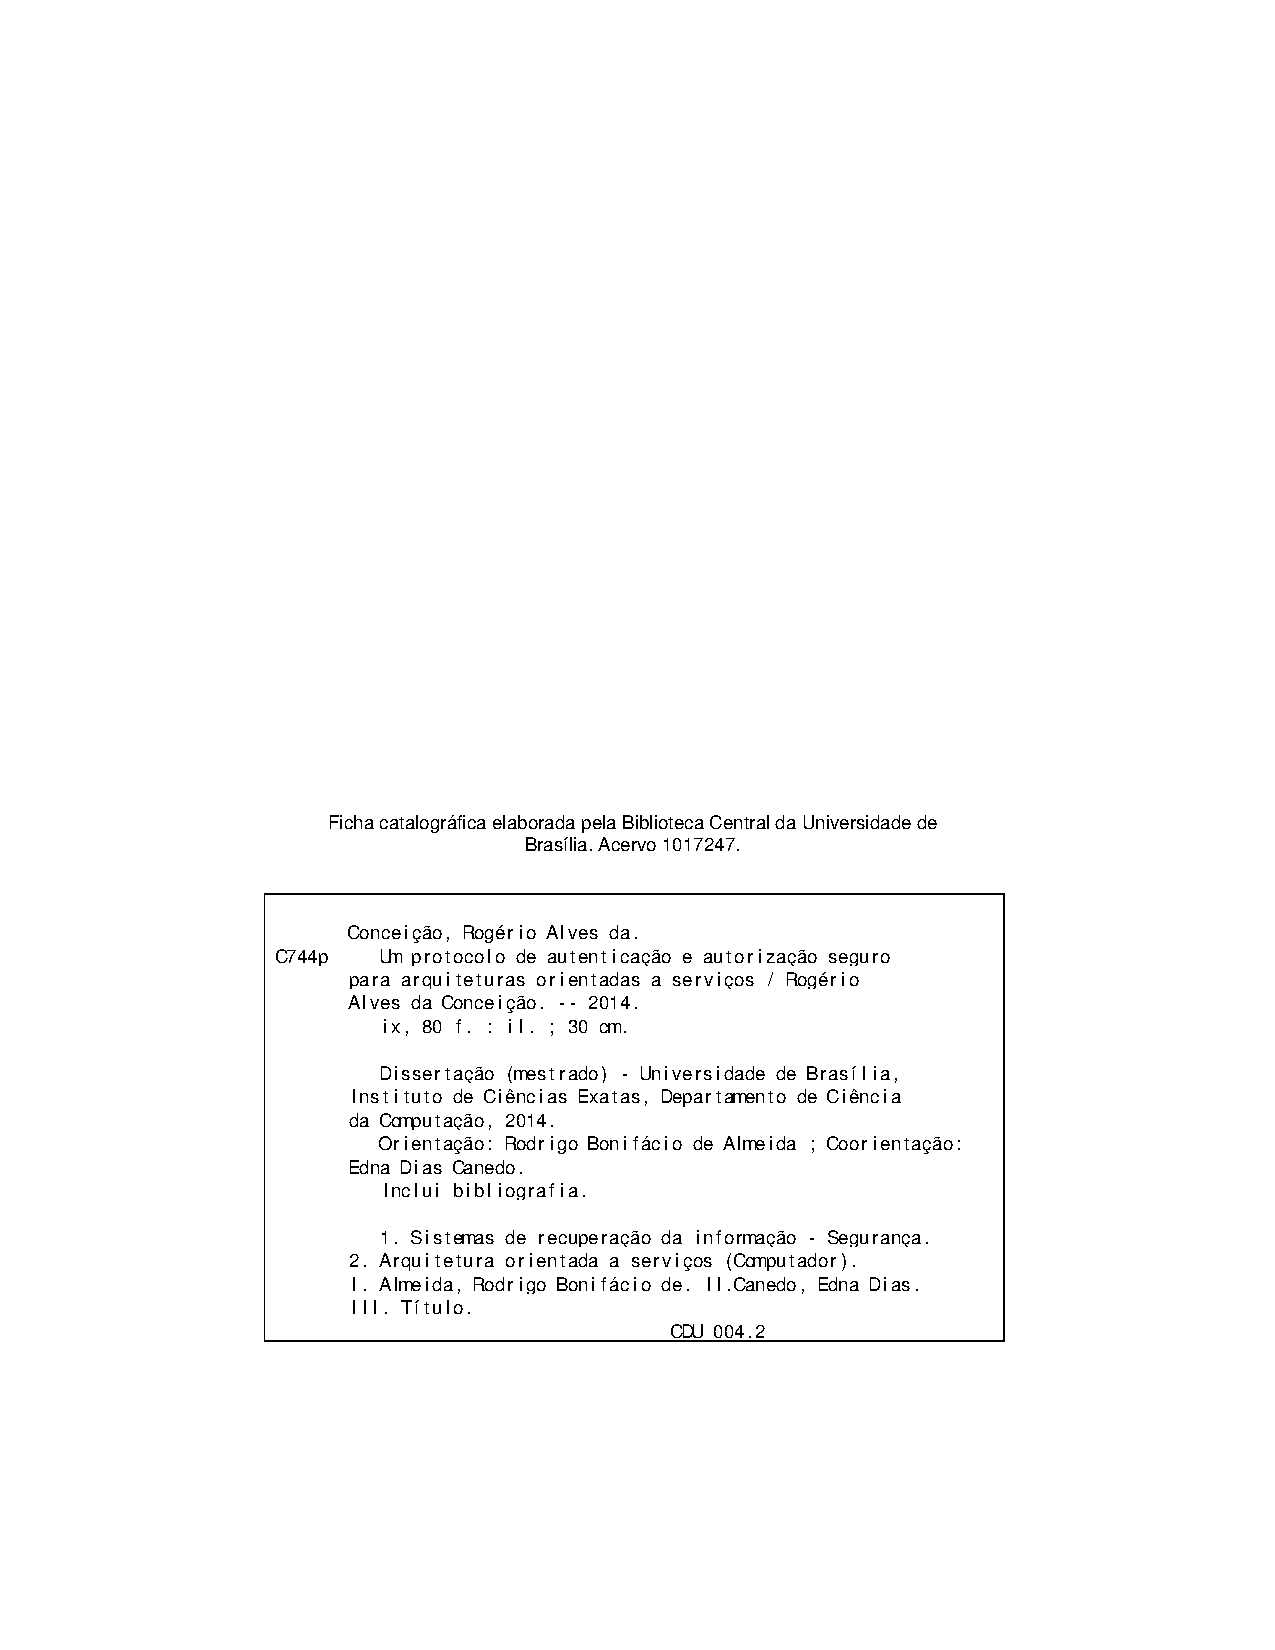
\includepdf[pages={1}]{tex/RogerioConceicao_1017247.pdf}
  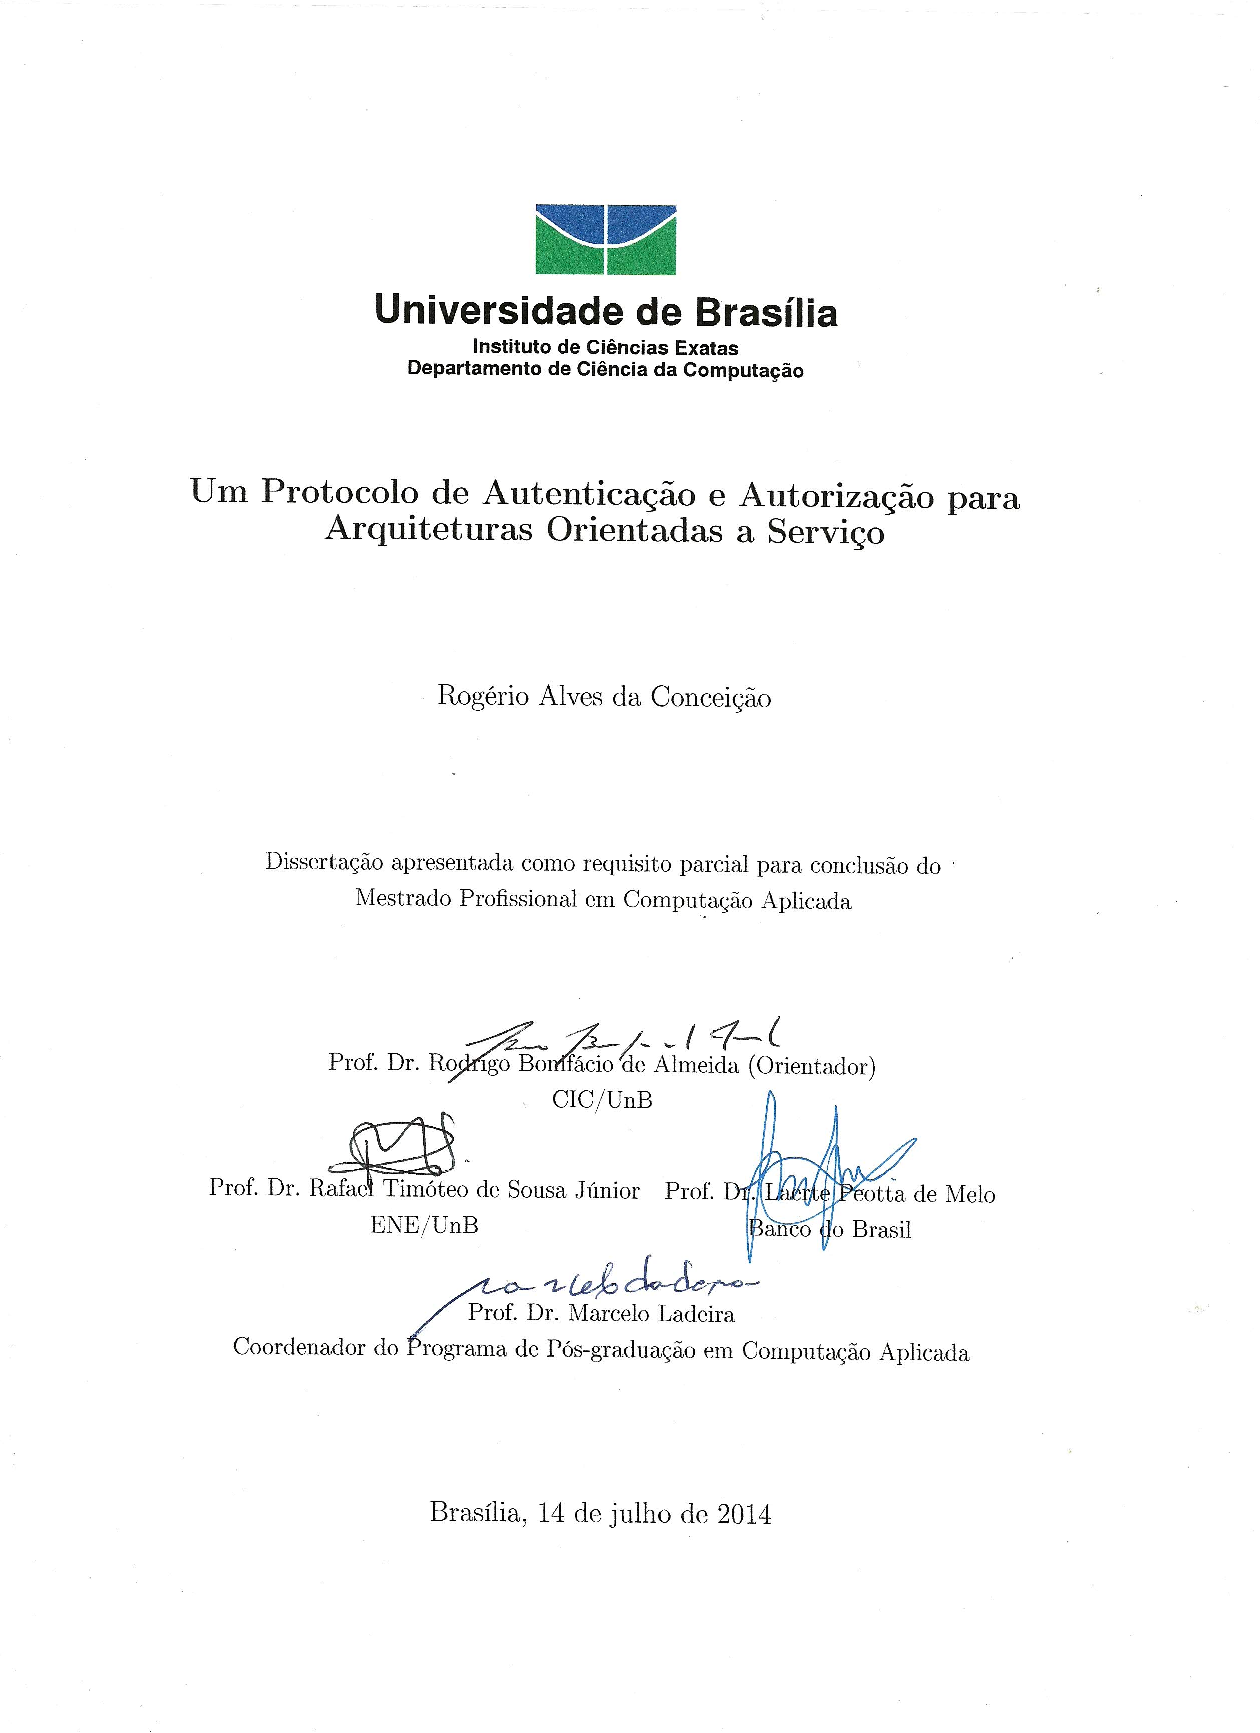
\includepdf[pages={1}]{tex/folhaAprovacao.pdf}
  \begin{dedicatoria}
  Dedico este trabalho à minha amada esposa Michelle e aos meus maravilhosos filhos Líris e Rafael, pelo apoio, incentivo e compreensão. Sem eles não teria conseguido concluir essa jornada.

  \end{dedicatoria}

  \begin{agradecimentos}
   Agradeço primeiramente a Deus que iluminou e guiou meus passos durante essa tragetória, me dando saúde e forças necessárias para superar as dificuldades ao longo do caminho.

   Aos meus orientadores, Prof. Dr. Rodrigo Bonifacio de Almeida e Profª. Drª. Edna Dias Canedo, pela orientação, apoio e confiança nesse período de amadurecimento e enriquencimento pessoal e intelectual. Serei eternamente grato por suas valiosas contribuições para a elaboração desta dissertação.

   Ao aluno Alexandre Lucchesi, do curso de Engenharia da Computação da UNB, pela contribuição valiosa dada a esta dissertação.

   Aos demais professores do Mestrado Profissional em Computação Aplicada, da Universidade de Brasília, pela competência com que transmitiram os conteúdos e ensinamentos.

   Aos companheiros de trabalho da Divisão de Tecnologia da Polícia Civil do Distrito Federal, que mesmo diante das correrias e obstáculos encontrados, sempre se dispuseram a me prestar o auxílio necessário.


  \end{agradecimentos}

\hyphenation{au-xi-li-ar}

\begin{resumo}
 A DITEC, Divisão de Tecnologia da Polícia Civil do Distrito Federal - (PCDF), tem como responsabilidade estratégica o desenvolvimento dos softwares da instituição, muitas vezes apresentando necessidades de integração e compartilhamento de informações sensíveis com órgãos conveniados. Dada a criticidade desses sistemas e informações compartilhadas, preocupações relacionadas a segurança devem ser tratadas sob uma perspectiva arquitetural dentro da instituição, que atualmente adota diferentes alternativas de integração, desde \emph{Web Services} até a replicação das bases de dados para instituições parceiras. Essa dissertação descreve  um protocolo de autenticação e autorização seguro, aderente a arquitetura \emph{Representational State Transfer} (REST), que tem como finalidade possibilitar que uma arquitetura orientada a serviços possa ser adotada como alternativa única de integração, balanceando os requisitos de segurança com outros atributos de qualidade,  em particular o tempo de processamento das requisições.

 O protocolo proposto foi especificado e analisado formalmente utilizando-se a lógica BAN. O protocolo é voltado para ambientes fechados, onde os potenciais clientes do serviço são conhecidos de forma antecipada e com isso torna-se viável o estabelecimento prévio de contratos para a utilização dos serviços ofertados pela Polícia Civil do Distrito Federal. Isso traz forte influência sob os mecanismos que podem ser usados no processo de autenticação e autorização.

 Com a realização deste trabalho foi possível realizar um mapeamento sistemático da literatura com a identificação e classificação dos trabalhos primários que discutem aspectos de segurança relacionados à computação orientada a serviços. Também foi definida uma arquitetura de referência que pode ser usada na integração de processos de negócio que podem envolver diferentes instituições utilizando computação orientada a serviços. Além disto, foram realizados testes automatizados em um protótipo funcional que permitiu investigar o impacto da adoção do protocolo em termos do custo adicional no tempo de resposta às requisições e \emph{throughput}.

\end{resumo}

\selectlanguage{american}
\begin{abstract}
 DITEC, Technology Division Civil Police of the Federal District, is responsible for the software's institution strategic development, often presenting needs of integration and sharing of sensitive information with government insured. Given the criticality of these systems and shared information, security concerns should be treated under an architectural perspective within the institution, which currently adopts different integration alternatives, from \emph{Web Services} to the replication of databases for partner institutions. This dissertation describes a secure protocol for authentication and authorization, adherent architecture Representational State Transfer(REST), which aims to enable a service-oriented architecture can be adopted as the sole alternative integration, balancing security requirements with other quality attributes, particularly time processing of requests.

 The proposed protocol is specified, and formally assessed using the BAN logic. The protocol is designed for closed environments, where potential customers of the service are known in advance and it becomes feasible the prior establishment of contracts for the use of services offered by Civil Police of the Federal District. This has a strong influence on the mechanisms that can be used in the authentication and authorization process.

 With this work it was possible to conduct a systematic mapping of literature with the identification and classification of primary studies that discuss security issues related to service-oriented computing. Was also defined a reference architecture that can be used in the integration of business processes that may involve different institutions using service-oriented computing. Besides this, automated tests were performed in a functional prototype which allowed to investigate the impact of the adoption of the protocol in terms the additional cost in response time to requests and throughput.

 \end{abstract}
\selectlanguage{brazil}
\hyphenation{a-tri-bu-tos}
  \tableofcontents
  \listoffigures
  \listoftables




\renewcommand{\appendixname}{Anexo}


  \textual

  %---------- Primeiro Capitulo ----------
\chapter{Introdução}\label{sec:introducao}
%\section{Apresentação}
As atribuições da Polícia Civil do Distrito Federal, no que diz respeito à sua competência de Polícia Judiciária, tangenciam em vários pontos as atribuições do Ministério Público do Distrito Federal e Territórios, do Tribunal de Justiça do Distrito Federal e Territórios e da Defensoria Pública do Distrito Federal. De forma que a competência de cada um desses Órgãos, por apresentarem pontos que se complementam, demanda intensa troca de informações.

A Polícia Civil do Distrito Federal, por meio de sua Divisão de Tecnologia, tem como propósito desenvolver seus próprios softwares. Esta atividade permite uma vantagem estratégica para a instituição, uma vez que a torna detentora dos softwares desenvolvidos evitando dessa forma a dependência tecnológica e administrativa de empresas privadas.

Nesse sentido, tem-se buscado estudar técnicas de desenvolvimento de software que promovam de forma efetiva a integração dos sistemas internos com os sistemas de Órgãos parceiros e que necessitem consumir de forma segura os dados e informações oriundos dos sistemas legados da Polícia Civil do Distrito Federal.

\section{Problema da pesquisa}

Nesse contexto, um dos principais desafios encontrados na DITEC refere-se à necessidade de integração e compartilhamento de informações de maneira segura, observando que as aplicações foram desenvolvidas em diferentes linguagens de programação e a integração ocorre com diferentes órgãos conveniados, tais como: Tribunal de Justiça do Distrito Federal e Território (TJDFT), Ministério Público da União (MPU), Departamento de Trânsito do DF (DETRAN-DF), Secretária de Segurança Pública do Distrito Federal (SSP-DF), Secretárias de Justiça do DF e Estados.

A ocorrência de uma vulnerabilidade de confidencialidade, por exemplo, ocorrendo o vazamento de informações sensíveis, criminosos poderiam utilizar essas informações e comprometer de forma significativa uma investigação policial.

Outra preocupação está relacionada à autenticidade, uma vez que todos os acessos a informações no âmbito da Polícia Civil do Distrito Federal devem ser realizados somente por pessoal autorizado. Caso isso não seja observado, pessoas podem se valer do anonimato e divulgar dados sigilosos de forma criminosa, o que também acarretaria inúmeros problemas de ordem jurídica para a instituição.

Dessa forma, devido à importância dessas informações, elas devem ter um tratamento diferenciado com relação a segurança nos aspectos de confidencialidade, autenticidade, integralidade e disponibilidade.

Por outro lado, na maioria das vezes, são disponibilizadas técnicas não seguras de integração, como a replicação ou o acesso direto a base de dados, apesar de existirem algumas iniciativas de integração baseadas em \emph{Web Services}.

No intuito de possibilitar que os sistemas possam ser integrados de forma eficiente e principalmente segura com outros sistemas, a Divisão de Tecnologia busca desenvolver uma metodologia própria que possa melhorar o processo integração de software no âmbito da Polícia Civil do Distrito Federal.
Para isso, optou-se pela utilização da Arquitetura Orientada a Serviços (SOA), que é um modelo arquitetural que propõem o uso de um conjunto de padrões para disponibilizar, descrever, publicar e invocar serviços. Neste cenário, este trabalho inicialmente propõe-se a investigar as seguintes questões de pesquisa:

\begin{enumerate}
	\item Quais são os principais problemas de segurança encontrados na adoção da Arquitetura Orientada a Serviços \-(SOA)? Essa questão de pesquisa é respondida nos capítulos 2 e 3 com o Mapeamento Sistemático e com a Revisão de Literatura.
	\item Quais padrões para construção de software seguro em arquiteturas SOA podem ser empregados pela Divisão de Tecnologia da Polícia Civil do Distrito Federal para realizar efetivamente a integração de seus sistemas com os sistemas dos órgãos parceiros? Neste caso, a resposta para essa questão é obtida no capítulo 3 com a Revisão de Literatura.
\end{enumerate}

Porém, posteriormente, após a proposição e o desenvolvimento do Protocolo de Autenticação e Autorização proposto, outras questões de pesquisa foram levantadas e investigadas. As questões são descritas a seguir:

\begin{enumerate}
\setcounter{enumi}{2}
  \item Qual o impacto observado no tempo de resposta às requisições com o uso do protocolo?
  \item Um protótipo funcional, sem foco em otimização, consegue suportar a demanda prevista?
\end{enumerate}  
  
Essas perguntas são respondidas no capítulo 5, com a realização de uma análise de desempenho do Protocolo de Autenticação e Autorização proposto.



\section{Justificativa}

Uma vez que a Polícia Civil do Distrito Federal desenvolva produtos de software mais seguros, que auxiliem no trabalho investigativo, ela realizará seu trabalho de uma forma mais efetiva, influenciando diretamente no combate da criminalidade e beneficiando a comunidade em geral e todos os órgãos distritais e federais tais como: Secretaria de Segurança Pública do Distrito Federal, Tribunal de Justiça do Distrito Federal, Ministério da Justiça, Secretarias de Governo Distritais, dentre outros órgãos, que necessitem das informações da instituição para realizar qualquer tipo de integração de software.

\section{Objetivos}\label{sec:Obj}
\subsection{Objetivo Geral}

Avaliar e aplicar o uso de técnicas, ferramentas  e procedimentos que garantam os requisitos de segurança em uma arquitetura orientada a serviços a ser usada para integrar os sistemas e automatizar os processos entre órgão parceiros (TJDFT, MPU, DETRAN, SSP).

\subsection{Objetivos Espec\'ificos}

\begin{enumerate}[a )]
	\item Realizar um mapeamento sistemático da literatura para compreender o estado da arte e da prática de segurança em SOA;

	\item Identificar e avaliar quais são os principais problemas de segurança encontrados na adoção da Arquitetura Orientada a Serviços (SOA);

	\item Estudar as especificações de Web Services relacionados a segurança e selecionar padrões e ferramentas para garantir confidencialidade, autenticidade e integridade nas integrações da arquitetura orientada a serviços. Essa seleção deve considerar o impacto na disponibilidade e no tempo de resposta dos serviços;

    \item Estabelecer uma arquitetura de referência na construção de software seguro em  SOA, por meio de um protocolo de autenticação e autorização, que possa ser empregado pela Divisão de Tecnologia da Polícia Civil do Distrito Federal para realizar efetivamente a integração de seus sistemas com os sistemas dos órgãos parceiros.

\end{enumerate}

\section{Organização do Trabalho}

Este trabalho está organizado em seis capítulos. No capítulo 2 é apresentado um mapeamento sistemático e os resultados obtidos com a sua realização. No capítulo 3 é realizada uma revisão da literatura onde são abordados os conceitos gerais sobre Arquitetura Orientada a Serviços (SOA), Web Services, REST, segurança e vulnerabilidades em SOA. Além disso, também são apresentados alguns protocolos de autenticação e autorização. No capítulo 4 é apresentado o protocolo de autenticação e autorização proposto e objeto deste trabalho. Neste capítulo são descritos os requisitos e a arquitetura do protocolo. É realizada uma análise formal do protocolo utilizando-se a lógica BAN. Neste capítulo também e descrita a implementação de um protótipo do protocolo proposto bem como uma análise de segurança. No capítulo 5 é realizada uma avaliação e análise de desempenho e são apresentados os resultados dos experimentos realizados. No capítulo 6 são apresentadas as conclusões do trabalho, bem como trabalhos futuros. 
  %---------- Terceiro Capitulo ----------
\chapter{Revisão de Literatura}\label{cap:revisaolit}
Este capítulo apresenta uma revisão dos principais conceitos relacionados ao tema deste trabalho, envolvendo Arquitetura Orientada a Serviço, Web Service, REST, Segurança Aplicada a SOA, Vulnerabilidades em SOA e Protocolos de Autenticação e Autorização.

\section{Arquitetura Orientada a Serviços}

%%A Arquitetura Orientada a Serviços (SOA) estabelece um modelo arquitetônico que visa aprimorar a eficiência, agilidade e a produtividade de uma empresa, posicionando os serviços como os principais meios para que a solução lógica seja representada no suporte à realização dos objetivos estratégicos associados à computação orientada a serviços \cite{ERL09}.

A Arquitetura Orientada a Serviços (SOA), consiste em uma coleção de componentes distribuídos que fornecem e ou consomem serviços~\cite{Clements2010}, tem sido amplamente utilizada por um grande número de empresas.

%Serviços correspondem a recursos de software bem definidos através de uma linguagem padrão, são auto-contidos,  proveem funcionalidades padrões do negócio, independentes do estado ou contexto de outros serviços~\cite{Furtado2009}.

SOA pode ser caracterizada como uma arquitetura corporativa onde serviços podem ser criados, reutilizados e facilmente compartilhados entre aplicações. Neste caso as funcionalidades de um sistema são decompostas em serviços interoperáveis o que permite a integração entre aplicações. O objetivo da SOA é estruturar sistemas distribuídos com base nas abstrações de regras e funções de negócio~\cite{Josuttis07}.

Existem muitas definições para SOA, no entanto elas possuem pontos em comuns pois em todos os conceitos são abordados temas que remetem ao compartilhamento do serviços, da independência da plataforma e linguagem de programação, da possibilidade de flexibilidade e agilidade no desenvolvimento de uma aplicação para gerenciar um negócio~\cite{ERL09}. O funcionamento de SOA baseia-se em três conceitos: serviços, interoperabilidade e baixo acoplamento~\cite{Josuttis07}.

Por serviços entende-se SOA como uma arquitetura neutra, que objetiva abstrair a realidade, concentra-se nos aspectos do negócio, possibilitando que sistemas sejam construídos em plataformas diferentes, tendo como finalidade a redução de problemas de integração, uma vez que isso  pode ser feito de forma flexível por meio dos serviços disponibilizados na arquitetura. Portanto, serviço pode ser visto como um conjunto de funções, abstrações de funcionalidades de negócios de um sistema com uma interface bem definida.

A interoperabilidade visa à integração entre esses sistemas e representa um objetivo fundamental da orientação a serviços, pois estabelece uma base para a realização de outros objetivos e benefícios estratégicos. Isso é possível, pois uma das características de SOA é que seus serviços são reutilizáveis, possuem baixo acoplamento, tem contratos formais e são independentes. Logo, uma vez que esses serviços estejam disponíveis aos clientes eles não precisam conhecer a lógica ou os processos de negócio para consumir e integrar serviços a suas aplicações.

O baixo acoplamento ou acoplamento fraco é um conceito vital para o funcionamento de um sistema distribuído, uma vez que ele determina que diferentes partes e funcionalidades de um sistema sejam independentes umas das outras, dessa maneira, alterações ou problemas em uma determinada parte do sistema não trará consequências para o resto do sistema, trazendo benefícios como escalabilidade, flexibilidade e tolerância a falhas. Acoplamento fraco refere-se a uma abordagem em que as interfaces podem ser desenvolvidas com o mínimo de suposições mútuas entre o emissor e os destinatários, reduzindo assim o risco de que uma mudança em um aplicativo ou módulo force uma mudança em outra aplicação ou módulo.

SOA é um estilo arquitetural e representa propositadamente uma tecnológica neutra. Para implementá-la podem ser usadas diversas tecnologias, como por exemplo: Web services, serviços REST-\emph{(Representational State Transfer)} e componentes distribuídos~\cite{erl2012soa}. Porém, atualmente as tecnologias mais empregadas para implementar SOA são os web services e os serviços REST, que são descritos nas seções~\ref{sec:webservice} e~\ref{sec:rest}, respectivamente.

\section{Web Services}\label{sec:webservice}

Web service pode ser definido como um sistema de software projetado para suportar interações interoperáveis máquina-a-máquina sobre uma rede~\cite{Booth2004}.

Um dos fatores da aceitação de Web services está no fato dele usar protocolos abertos de comunicação na Internet e XML para transacionar o seu negócio. Um Web service é, portanto, um sistema de software que pode agir a pedido de qualquer computador conectado à rede e que se comunica usando padrões XML~\cite{Pulier2005}.

Por meio desta tecnologia é possível promover a interoperabilidade entre aplicações e que tenham sido desenvolvidos em plataformas diferentes tornando-as compatíveis permitindo que as aplicações enviem e recebam dados em formatos variados. Cada aplicação pode ter a sua própria linguagem, que é traduzida para uma linguagem universal, como é o caso do formato XML.

A abordagem de arquiteturas orientadas a serviço e Web services estão centradas no conceito de serviço, tanto a nível de negócios  quanto a nível tecnológico, e compartilham os mesmos princípios~\cite{Bertino2010}. Dentre os princípios que mais se destacam podem ser citados:

\begin{itemize}
    \item Autonomia de serviço: Para os serviços realizarem suas capacidades de modo consistente e confiante, sua lógica precisa ter um grau significativo de controle sobre seu ambiente e recursos~\cite{ERL09}.

    \item Baixo acoplamento: Acoplamento refere-se a uma conexão do relacionamento entre dois elementos. Uma medida de acoplamento se compara a um nível de dependência~\cite{ERL09}. De outra forma pode dizer que o baixo acoplamento refere-se a uma abordagem em que as interfaces podem ser desenvolvidas com a mínima dependência uma das outras o que reduz o risco  de uma mudança e qualquer uma das partes forçar a mudança na outra parte não modificada.

    \item Contrato formal: O contrato informa o que o Serviço faz e como ele se comunica (o que deve receber e o que deve entregar). Em outras palavras, Contratos são documentos textuais que descrevem o que o serviço faz e eles são o foco do design de serviço, porque regem praticamente tudo que é feito pelos serviços~\cite{ERL09}. Logo, todo serviço possui um contrato entre o requisitante e o provedor deste serviço.

\end{itemize}

Segundo~\cite{Bertino2010}, cada organização tem que ter autonomia para exercer um controle independente sobre os seus serviços. Para isso a autonomia do negócio tem que ser correspondente a do Web Service no momento do oferecimento e execução do serviço.

A plataforma de Web services é definida por vários padrões da indústria suportados por todas as comunidades de fornecedores. Essa plataforma está associada à coleção de padrões e especificações de tecnologias abertas tais como Simple Object Access Protocol (SOAP), Web Services Description Language (WSDL) e  Universal Description and Discovery Information (UDDI). Nas seções a seguir será feito uma descrição de cada uma dessas tecnologias.


\subsection{Simple Object Accesss Protocol (SOAP)}
SOAP é um protocolo de transporte que é responsável pela troca de mensagens entre aplicações em ambientes distribuídos e descentralizados, ele segue um padrão que foi especificado pelas normas da W3C, sendo baseado em XML o que o torna totalmente compatível com qualquer plataforma e com linguagens que tenham suporte para a manipulação de arquivos XML. Seu conteúdo é composto por informações e estruturas de dados~\cite{COYLE}.

A estrutura de uma mensagem SOAP é definida em um documento XML, sua estrutura possui os seguintes elementos:\emph{ envelope, body} que são obrigatórios e \emph{header e fault} que são opcionais. As seguir uma breve descrição desses elementos:

 \begin{itemize}
            \item \emph{Envelope}: Este é o elemento raiz da mensagem SOAP sendo responsável por identificar o documento XML com uma mensagem SOAP e por definir o conteúdo da mensagem;

            \item \emph{Header} (opcional): Contêm os dados do cabeçalho, este elemento possui informações especificas do aplicativo da mensagem SOAP;

            \item \emph{Body}: Contém as informações de chamada e resposta ao servidor, ele contém a mensagem SOAP pretendida que o usuário espera;

            \item \emph{Fault}: Este elemento possui as informações dos erros ocorridos no envio da mensagem. Esse elemento só aparece nas mensagens de resposta do servidor.

 \end{itemize}


\subsection{Web Services Description Language (WSDL)}

Web Services Description Language (WSDL) é uma linguagem para descrição de serviços escrita em XML. São descritos os serviços externos, ou interfaces que são oferecidos por uma determinada aplicação, independente de sua plataforma ou linguagem de programação. Além disso, contém as especificações de localização das operações (métodos ou serviços) que fazem parte dos Web Services. Atualmente, encontra-se na versão 2.0.

WSDL podem ser mapeados para qualquer linguagem de implementação, plataforma, modelo de objeto e ou sistema de mensagens~\cite{Bertino2010}. É caracterizado por uma parte abstrata, onde é descrita a interface do serviço e outra concreta local onde são definidos os protocolos de conexão e outras informações, conforme Figura~\ref{fig:composicao_WSDL}.

A parte abstrata é constituída pelos seguintes elementos: Tipos, que são elementos que definem os tipos de dados usados pelos Web Services, neles são especificados os tipos que serão trocados nas mensagens de entrada e saída do serviço; Mensagem, que é um elemento que permite descrever de forma abstrata os dados que serão transmitidos entre o serviço e o consumidor do serviço; Operações, que é um elemento que é semelhante à definição de um método, no entanto, só permite que seja definido a entrada, saída e mensagens de erro que estão associados com uma operação e PortType, que são conjuntos de operações abstratas, que são suportadas por um serviço, cada um contendo mensagens de entrada e saída.

A parte concreta do WSDL, local de definição do protocolo e do endereço onde o serviço estará disponibilizado, compõe-se pelos seguintes elementos: O binding (ligação), que é o elemento que é responsável por ligar os elementos abstratos e concretos em um documento WSDL e de fornecer detalhes de como as mensagens serão transmitidas. E os Serviços e Portas, que são elementos que especificam a localização (endereço URL ou e-mail), neste caso, o elemento de serviço atribui um nome para o serviço e o associa a uma interface abstrata e descrevendo o local onde o serviço será acessado.

\begin{figure}[!htb]
\centering
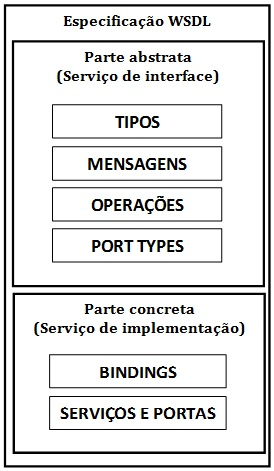
\includegraphics[scale=0.5]{COMPOSICAO_WSDL.jpg}
\caption{Especificação de serviços WSDL, adaptado de~\cite{Bertino2010}.}
\label{fig:composicao_WSDL}
\end{figure}


\subsection{Universal Description, Discovery and Integration (UDDI)}

UDDI é um componente importante da arquitetura de Web Services, sendo formado por um serviço de diretório que armazena descrições de serviço. Esse serviço obedece ao padrão integração, descoberta e descrição universal. Além disso,  ele prescreve o layout de um banco de dados que contém  descrições de serviços que permitirão a clientes de serviços web procurar serviços relevantes~\cite{TANENBAUM2007}.

O UDDI provê um método padronizado para a publicação e descoberta de informações, permitindo que as empresas tanto publiquem como encontrem Web Services. Segundo~\cite{Cerami2002}, os dados capturados dentro de UDDI são divididos em três categorias principais:

\begin{enumerate}[a )]
	\item Páginas brancas: Esta categoria inclui informações gerais tais como nome, descrição e endereço dentre outras informações sobre o fornecedor do serviço;

	\item Páginas amarelas: Esta categoria inclui dados de classificação geral para qualquer empresa ou serviço oferecido. Por exemplo, esses dados podem incluir a indústria, o produto, ou códigos geográficos baseados sobre taxionomias padronizadas;

	\item Páginas verdes: Esta categoria inclui informações técnicas sobre um Web Service. Geralmente, essa informação inclui um apontador (ponteiro) para uma especificação externa e um endereço para invocar o serviço.

\end{enumerate}

\section{Representational State Transfer}\label{sec:rest}
A arquitetura \emph{Representational State Transfer} (REST), foi proposta por Roy Fielding em
2000 em sua tese de doutorado e pode ser descrita como um conjunto de princípios arquiteturais que podem ser utilizados para o desenvolvimento de serviços web e que utilizam o protocolo HTTP para realizar as trocas de mensagens~\cite{ Fielding2000}.

Dessa forma, para que os princípios arquiteturais que permeiam REST sejam seguidos, um conjunto de restrições deve ser implementado~\cite{ Fielding2000}. Uma aplicação que esteja em conformidade com essas restrições, a seguir descritas, são classificadas com RESTful~\cite{Richardson2007}.

\textbf{Cliente-Servidor:} Essa restrição está associada a separação de interesses, que é o princípio por trás das restrições da arquitetura cliente-servidor. Procura-se separar as preocupações relacionadas à interface do usuário das preocupações de armazenamento de dados. Isso permite que os componentes possam evoluir de forma independente melhorando a portabilidade e a escalabilidade das aplicações.

\textbf{\emph{Stateless}:} Diz respeito à interação entre cliente e servidor. Nesse caso, a  comunicação deve ser realizada sem que haja o armazenamento de qualquer tipo de estado no servidor. Sendo assim,  toda informação de estado deve ser conhecida somente pelo cliente.  Esta característica permite a escalabilidade do servidor, uma vez que pode liberar recursos no final de cada pedido.
Contudo, uma desvantagem associado a essa característica  está relacionada à performance da rede, pois em decorrência das constantes requisições com dados repetidos  ela é reduzida.

\textbf{\emph{Cache}:} A utilização do cachê, tem  a finalidade de diminuir o impacto da desvantagem ocasionada pela redução de performance. Uma vez que exige que os dados de uma resposta vinda de uma requisição ao servidor, sejam marcados como \emph{cacheable} (sujeito à utilização do cachê) ou \emph{noncacheable} (não sujeito à utilização do \emph{cache}). Se uma resposta for marcada como \emph{cacheable}, então ela será reutilizada como resposta em futuras requisições equivalentes, permitindo que o servidor fique mais livre, e portanto, mais escalável, haja vista que algumas interações poderão ser eliminadas por completo, o que melhora a eficiência e performance de acesso a recursos percebido pelo usuário.

\textbf{Sistema em camadas:} Essa restrição caracteriza-se pela divisão do sistema em camadas hierárquicas, restringindo a visualização dos componentes participantes de forma que cada componente só possa ver a camada com a qual esteja interagindo diretamente. Ao restringir a visibilidade de um sistema a uma única camada, torna-se possível delimitar a complexidade do sistema e promover a independência de cada uma das camadas.  Essa separação permite que  o sistema seja mais robusto e resistente a erros.

\textbf{Code-On-Demand:} Dentre o conjunto restrições propostas pelo estilo REST, esta é a que permite a opção de baixar e executar diretamente códigos no lado cliente, sendo opcional. Com isso, busca-se  obter extensibilidade e simplificar  o cliente. No entanto, isso também reduz a visibilidade.

\textbf{Interface Uniforme:} A principal característica que diferencia o estilo arquitetural REST de outros utilizados em rede é a ênfase  quanto ao uso de uma interface uniforme entre os componentes. Aplicando o princípio de generalização de engenharia de software à interface dos componentes, a arquitetura é simplificada e a visibilidade das interações é melhorada. Contudo, esta generalização pode diminuir a eficiência do sistema, devido à aplicação não poder transmitir a informação em um formato específico de acordo com a sua  necessidade. Com o objetivo de obter uma interface uniforme, REST define quatro requisitos de interface:

 \begin{itemize}
    \item \textbf{Identificação dos recursos:} Na arquitetura REST, cada recurso deve possuir um identificador universal denominado \emph{Uniform Resource Identifier} (URI). Que é definido como uma sequência de caracteres que identificam um recurso físico ou abstrato~\cite{bernerslee2005uri}. E são utilizados para descoberta de recursos e serviços.
    \item	\textbf{Representação de recursos:} Os recursos devem ser manipulados a partir de suas representações, uma vez que podem estar representadas em formatos diferentes formatos, tais como: JSON, XML,PDF, texto puro, etc. É importante frisar que uma aplicação REST não transmite o recurso efetivamente, mas sim a sua representação, em um formato pré-acordado entre o cliente e o servidor.
    \item	\textbf{Mensagem auto descritivas:} Os recursos são dissociados da sua representação, haja vista que o seu conteúdo  pode que ser acessado em formatos diferentes. Dessa forma, as mensagens devem conter metadados que indicam como o conteúdo transmitido deve ser tratado.  Os metadados são utilizados para controlar cache, detectar erros de envio, negociar formatos de uma representação adequada, realizar controle de autenticação e acesso, etc.
    \item	\textbf{Utilização de hipermídia para estado da aplicação:} Neste caso, as representações de recursos obtidas em uma aplicação REST devem possuir \emph{hiperlinks} que permitam a navegação do cliente pelos recursos. Uma vez que o servidor não pede  armazenamento de qualquer tipo de estado. Dessa forma, o Cliente pode interagir com outros recursos existentes sem a necessidade de que ele conheça a relação completa destes recursos pois poderá seguir estas ligações para se deslocar de um recurso para outro.


    %Este pré-requisito é o menos cumprido por aplicações autointituladas RESTful: As representações de recursos obtidas em uma aplicação REST devem possuir hiperlinks que permitam a navegação do cliente pelos recursos. Ou seja, diferentemente de arquiteturas baseadas em RPC (Remote Procedure Call), o cliente não deve conhecer previamente as URIs para os recursos da aplicação (apenas a raiz do serviço), sendo que o servidor deve prover links que permita a descoberta dos recursos pelo cliente; não há contrato do serviço e não há garantia que um recurso em uma determinada URI possa estar disponível no futuro;
\end{itemize}

O protocolo HTTP é o padrão utilizado na arquitetura REST para promover a comunicação entre o cliente e o servidor. Isso se dá pela manipulação dos recursos utilizando os métodos HTTP: GET, POST, PUT, DELETE E e adicionalmente os métodos HEADER e OPTIONS.

Neste contexto, o método GET é utilizado para recuperar uma representação de um recurso.O metódo PUT para criar um novo recurso ou modificar um existente, DELETE é utilizado para remover um recurso e POST é comumente utilizado para criação de um novo recurso. HEADER é empregado para recuperar metadados de uma representação, podendo ser usado para empregar melhoria no cache. OPTIONS que retornar uma descrição de serviço ou explicação dos métodos disponíveis de uma determinada URI.
%verificar
%Os métodos HTTP descritos podem ser classificados quanto a segurança e idempotência. De forma que uma solicitação é considerada segura, quando o método utilizado não altera o estado do recurso. E  idempotente, se o resultado de uma solicitação realizada com sucesso é independente do número de vezes que é executada (RICHARDSON, 2007)

%Os métodos GET, HEAD e OPTIONS são seguros e idempotentes, pois não alteram o estado do recurso.  PUT e Delete não são seguros, mas são idempotentes. O método POST é o único método que não é seguro nem idempotente.  (RICHARDSON, 2007)


%

Os serviços web que são desenvolvidos baseados na arquitetura REST, ou seja, serviços Web RESTful  são relativamente simples, pois a arquitetura REST segue padrões W3C/IETF3 bem conhecidos tais como (HTTP, XML, URI, MIME). Além disso, a sua adoção não é difícil de ser implantada, pois pode ser implementada em várias linguagens e em diferentes sistemas operacionais~\cite{Pautasso2008}.

Serviços Web RESTful, são escaláveis e oferecem suporte a cache através do protocolo HTTP, \emph{clustering} e balanceamento de carga. Outra vantagem é a possibilidade de otimização de desempenho de web services, uma vez que podem utilizar formatos de mensagem mais leves, como por exemplo, o \emph{JavaSript Objetc Notation}(JSON)~\cite{Pautasso2008}.


\section{Segurança em SOA}

\subsection{Conceitos Básicos}

Segurança da informação pode ser definida como um conjunto de ações que são executadas com a finalidade de prover segurança às informações de indivíduos e organizações. Atualmente, a segurança é um requisito importante para qualquer aplicação distribuída, tais como aplicações governamentais, aplicações de segurança pública e de defesa dentre outros~\cite{Bertino2010}.

A segurança aplicada a SOA requer o estabelecimento de propriedades básicas, uma vez que os aspectos funcionais aplicados a esta arquitetura são iguais aos de aplicações tradicionais.  Logo, segundo~\cite{Verissimo2001}, a segurança está fundamentada nos seguintes atributos básicos: autenticidade, integridade, confidencialidade e disponibilidade.

No que se refere à autenticidade, este é um atributo que visa estabelecer a origem da informação, buscando verificar a identidade de um usuário. Assim, objetiva-se garantir que o usuário ou serviço é realmente quem diz ser e que tem os privilégios necessários para acessar e ou enviar uma determinada informação.

A integridade é aquela que se preocupa em evitar ou em detectar a modificação não autorizada de informações ou mensagens. Esse atributo busca proteger a mensagem de modificações não permitidas.

A confidencialidade preocupa-se com a proteção contra acessos não autorizados de dados e informações. Segundo~\cite{Bertino2010}, esse atributo procura proteger o conteúdo de uma mensagem ou informação  para que ele não possa ser visualizado no momento da transmissão, exceto por serviços autorizados a visualizá-los por terem a necessidade de ver o conteúdo da mensagem, a fim de realizar o seu encaminhamento.

Finalmente, a disponibilidade está preocupada com a garantia de que os serviços de informação permaneçam acessíveis somente a usuários autorizados. De forma que uma mensagem ou informação uma vez solicitada possa ser prontamente entregue ao destinatário, garantindo assim que os usuários legítimos recebam os serviços a que têm direito. Em outras palavras, esse atributo busca garantir que a informação estará disponível quando solicitada.

Apesar de compartilhar estes conceitos,  a segurança em SOA exige uma abordagem  diferenciada e outros aspectos devem ser verificados. Um exemplo disto é a proposta de segurança em nível de mensagem.

Segundo~\cite{SOASecurity2008}, a segurança em nível de mensagem busca sanar problemas e complementar a segurança que é oferecida na camada de transporte, que é realizada por meio dos protocolos SSL (\emph{Security Socker Layer}) e TLS (\emph{Transport Layer Security}). Neste caso, os dados são cifrados na camada de transporte sendo estabelecido um canal seguro de comunicação entre dois serviços. Dessa forma, a comunicação ponto a ponto é garantida e segura. Porém, uma vez existindo interfaces intermediárias entre provedor do serviço e o consumidor, o processo de cifrar e decifrar os dados, que ocorre na camada de transporte, irá ocorrer toda vez que os dados trafegarem por um serviço intermediário, isso faz com que o sigilo dos dados e a segurança sejam quebrados em cada serviço intermediário. Para resolver este problema, propõem-se a segurança em nível de mensagem que consiste em utilizar mecanismos de segurança como cifrar partes da mensagem, o que resolve este problema, pois a segurança é fim a fim o que significa dizer que os dados estarão seguros mesmo quando a transmissão envolver um ou mais intermediários.

\subsection{Criptografia}

A palavra criptografia origina do Grego kryptós, ``escondido'', e gráphein, ``escrever'',  e pode ser  conceituada como sendo a ciência e a arte de manter mensagens seguras~\cite{Schneier1995}. Ela está  associada a vários aspectos da segurança da informação, tais como: privacidade ou confidencialidade, integridade do dados, autenticação e não-repúdio~\cite{Menezes1996}. Em síntese, o processo de criptografia consiste em transformar uma informação que está em texto claro (\emph{plaintext}), em uma informação cifrada (\emph{ciphertext}), criptografada. O processo inverso, que é o de transformar uma informação cifrada em um texto claro, não codificado é denominado decriptografia. A Figura~\ref{fig:processocriptografia} exemplifica esse processo.

\begin{figure}[!htb]
\centering
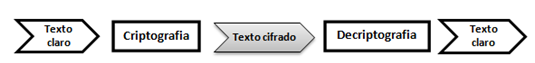
\includegraphics[width=0.8\textwidth]{processocriptografia.png}
\caption{Relação entre os termos  básicos de criptografia adaptado de~\cite{Schneier1995}.}
\label{fig:processocriptografia}
\end{figure}

Para realizar o processo de criptografia é necessário a utilização de um sistema criptográfico que é formado pelo conjunto de textos em claro, textos cifrados e chaves. Atualmente existem dois tipos de sistemas criptográficos: o de chave simétrica e o de chave assimétrica.

\subsection{Criptografia de Chave Simétrica}

A criptografia de Chave Simétrica pode ser definida como sendo aquela que utiliza uma chave única tanto para cifrar quanto para decifrar um texto claro~\cite{stallings2008}. Esse sistema de criptografia possui basicamente cinco elementos: Texto claro, que é a mensagem original; Algoritmo de criptografia, que o responsável por realizar as transformações no texto claro; A chave secreta, que é a chave compartilhada entre o emissor da mensagem e o receptor, utilizada como entrada para o algoritmo de criptografia; Texto cifrado, que é a mensagem em que foi aplicada o algoritmo criptográfico, é a saída e algoritmo de criptografia: Que é basicamente o mesmo algoritmo de criptografia só que executado de forma inversa. Para isso, ele aplica ao texto cifrado a chave secreta compartilhada, utilizada no momento da cifragem, e obtém o texto claro original. O processo do Sistema Criptografia de Chave Simétrica é ilustrado na figura~\ref{fig:criptografiasimetrica}

\begin{figure}[!htb]
\centering
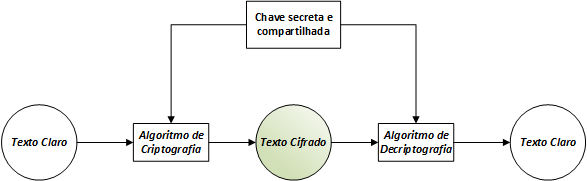
\includegraphics[width=0.9\textwidth]{criptosimetrico.png}
\caption{Processo de criptografia simétrica adaptado de ~\cite{stallings2008}.}
\label{fig:criptografiasimetrica}
\end{figure}

Existem dois tipos de algoritmos de criptografia de chave simétrica: os de cifras de fluxo e cifras de blocos. Cifras de fluxo, cifram e decifram dados bit a bit, ou seja, um bit a cada unidade de tempo, não sendo muito adequado a implementações em software. Já a cifras de blocos, realizam as mesmas operações em blocos de bits, sendo mais fáceis de implementar em softwares~\cite{Schneier1995}. São exemplos de algoritmos de criptografia de chave simétrica: AES(Advanced Encryption Standard), BlowFish, Triple-DES e DES (Data Encryption Standard).



\subsection{Criptografia de Chave Assimétrica}

A criptografia de Chave Assimétrica ou de chave pública é aquela que utiliza uma chave para criptografia e outra chave diferente, porém relacionadas matematicamente, para decriptografia~\cite{stallings2008}. Dessa forma, cada usuário possui um par de chaves, uma pública e outra privada, que são utilizadas no processo de ciframento e deciframento das mensagens. Na utilização dessa técnica, todos os participantes têm acesso a chave pública porém as chaves privadas devem ser de conhecimento apenas do seu proprietário, devendo permanecer protegida e secreta~\cite{stallings2008}. A figura~\ref{fig:criptografiaassimetrica} exemplifica o processo de Criptografia de Chave Assimétrica.

\begin{figure}[!htb]
\centering
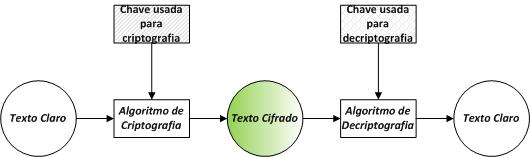
\includegraphics[width=0.9\textwidth]{criptografiaassimetrica.png}
\caption{Processo de criptografia assimétrica.}
\label{fig:criptografiaassimetrica}
\end{figure}

A criptografia assimétrica ou de chave pública pode ser utilizada tanto para prover a confidencialidade como para possibilitar a autenticidade da mensagem. Quando usada para prover a confidencialidade dos dados, a mensagem é criptografada com a chave pública do receptor e só pode ser decifrada com a chave privada do destinatário. Vários algoritmos de criptografia de chave pública foram propostos, porém os que mais se destacaram  tanto para  criptografia quanto para assinaturas digitais foram o RSA, ElGamal e Rabin~\cite{Schneier1995}.

\subsection{Funções de Hash}
Uma função de \emph{hash} é aquela que ao ser aplicada a uma mensagem de comprimento variável, produz como saída um valor \emph{hash}, de tamanho fixo~\cite{Schneier1995}, também chamado de resumo de mensagem. É amplamente utilizada em aplicações criptográficas, tais como: assinaturas digitais, esquemas de proteção de senha e autenticação de mensagens. A finalidade da função de \emph{hash} é produzir um identificador único em um arquivo, mensagem ou bloco de dados. Para isso, ela deve satisfazer aos seguintes requisitos~\cite{stallings2008}:
\begin{itemize}
\item H pode ser aplicado a um bloco de dados de qualquer tamanho.
\item H produz uma saída de comprimento fixo.
\item Dado uma mensagem qualquer de entrada, deve ser fácil calcular o seu valor hash.
\item Para qualquer valor \emph{hash}(h) dado, é computacionalmente inviável encontrar x tal que H(x)= h. Ou seja,  deve ser resistente a primeira inversão, de forma que seja fácil gerar um código dada uma mensagem, mas muito difícil gerar um mensagem dado um código.
\item Para qualquer bloco dado x, é computacionalmente inviável encontrar y diferente x, tal que H(y)= H(x). Isso é conhecido como resistência fraca a colisões.

\item É computacionalmente inviável encontrar qualquer par(x,y) tal que H(x)= H(y). Ou seja, deve possuir resistência forte a colisões.

\end{itemize}

Vários algorimos de \emph{hash} foram desenvolvidos ao logo dos anos. Como exemplo podem ser citados os algoritmos de resumo criptográfico ou MD(\emph{Message Digest}), desenvolvidos por Ron Rivest, e cuja a última versão foi o MD5. Porém a funções de \emph{hash} da familia MD foram considerados inseguros e devem ser evitados~\cite{forouzan2013redes}.

Outro exemplo, que merece destaque, são os algoritmos de hash seguro(SHA - \emph{Secure Hash Algorithm}). Eles foram desenvolvidos como alternativa a insegurança dos algoritmos MD(\emph{Message Digest}). O SHA é um padrão desenvolvido pelo Instituto Nacional de Padrões e Tecnologia (NIST-\emph{National Institute of Standards and Technology}). Atualmente, o SHA, encontra-se na versão 3,(SHA-3), sendo considerado o padrão recomendado para aplicações atuais e futuras~\cite{forouzan2013redes}.

\subsection{Assinatura Digital}

A assinatura digital pode ser definida como o mecanismo de autenticação que permite que o criador de uma mensagem possa anexar um código que atue como assinatura e garanta origem e integridade da mensagem~\cite{stallings2008}. As assinaturas digitais podem ser geradas tanto por sistemas criptográficos assimétricos, usualmente os mais empregados, quanto simétricos. No caso da geração da assinatura digital com sistemas criptográficos assimétricos, o processo ocorre da seguinte maneira: a mensagem é criptografada com a chave privada do remetente, de forma que qualquer pessoa que possua a chave pública do remetente possa verificar a autenticidade da mensagem.

Porém a utilização da criptografia assimétrica é lenta, e como alternativa utiliza-se a combinação dos sistemas criptográficos com as funções de \emph{hash}. O que torna o processo mais rápido. Isso ocorre porque não se criptografa toda mensagem e sim apenas o resumo criptográfico, que é o resultado da aplicação da função de hash sobre a mensagem. Assinar um resumo criptográfico não é apenas mais eficiente do que assinar a própria mensagem, mas também uma defesa contra ataque do homem-do-meio, descritos na seção 3.5.4~\cite{goodrich2013}.

Dessa forma, para gerar uma assinatura digital, utilizando a combinação da criptografia assimétrica com a função de \emph{hash}, deve-se seguir os seguintes passos, conforme descrito na figura~\ref{fig:esquemaassinaturadigital}. O emissor da mensagem aplica uma função de hash na mensagem que deseja enviar a um receptor, criando dessa forma, um resumo da mensagem com tamanho fixo. Em seguida, o emissor criptografa esse resumo com a sua chave privada e envia ao receptor juntamente com a mensagem original. O receptor, por sua vez, recebe o documento e realiza o processo de verificação da assinatura, de forma a determinar a autenticidade e integridade da mensagem enviada. Para realizar essa verificação, ele aplica a mesma função de hash utilizada pelo emissor na mensagem original, e na sequência, o receptor utiliza a chave pública do emissor para decifrar o resumo de mensagem enviado, se o valor de \emph{hash} gerado pelo receptor  for igual ao valor de \emph{hash} enviado então o receptor terá a certeza que o documento não foi adulterado e que ele foi enviado realmente pelo emissor, detentor da chave privada. Em outras palavras a assinatura digital é válida.

\begin{figure}[!htb]
\centering
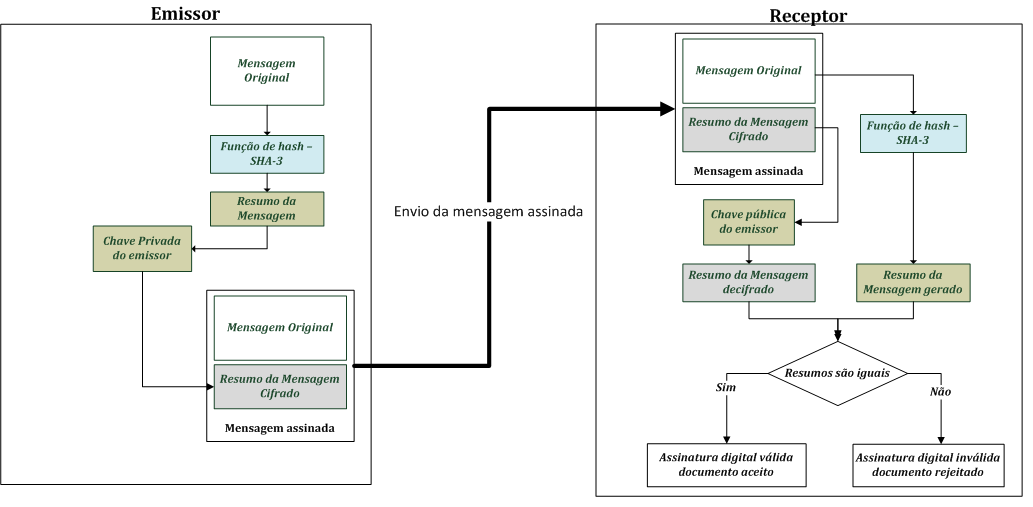
\includegraphics[width=0.9\textwidth]{esquema_assinatura_digital.png}
\caption{Processo de assinatura digital com função de hash.}
\label{fig:esquemaassinaturadigital}
\end{figure}

\subsection{Certificados Digitais}

Um certificado digital é um documento eletrônico que possui informações que comprovam a identidade do seu emissor. Esse documento eletrônico é gerado e assinado por uma terceira parte confiável, denominada Autoridade Certificadora (CA). Uma CA é responsável por associar uma chave pública a uma entidade(pessoa, processo, servidor etc)~\cite{forouzan2013redes}. Dessa forma, uma das finalidades de um certificado digital é garantir que a chave pública contida no certificado pertence à entidade à qual ele foi emitido, possibilitando assim, a identificação inequívoca das partes envolvidas em uma comunicação.

O padrão inicialmente adotado para os certificados digitais foi esquema X.509 que é uma recomendação do ITU-T(\emph{International Telecommunication Union}) e faz parte da série de recomendações X.500, que definem um serviço de diretório que mantém informações sobre usuários~\cite{stallings2008}.

Um certificado digital X.509 normalmente contém os seguintes campos:

 \begin{itemize}

\item Versão: Diferencia entre versões sucessivas do formato de certificado; V1, V2, V3 ou, designando a versão padrão do certificado.

\item Número de série: Um número único de série emitido por uma CA que identifica o certificado.
\item Identificador do algoritmo de assinatura: O algoritmo usado pela CA para assinar o certificado.
\item Nome do emissor: Um identificador exclusivo para a autoridade certificadora que emitiu o certificado.
\item Validade: Início e fim do período de validade do certificado.
\item Nome do titular:  Um nome único que identifica a entidade para a qual o certificado foi emitido.
\item Informações de chave pública do titular: Contém a chave pública para a entidade identificada juntamente com um identificador para o algoritmo de criptografia usado com a chave (próximos dois itens).
\item Algoritmo de assinatura: Especifica o algoritmo utilizado pela CA para assinar o certificado.
\item Assinatura: Abrange todos os outros campos do certificado; contém o código hash dos outros campos, criptografafados com a chave privada da CA.
\item Identificador exclusivo do emissor(opcional): Um identificador exclusivo usado para identificar o CA emissor caso o nome X.500 tenha sido reutilizado para entidades diferentes.
\item Identificador exclusivo do titular (opcional): Um identificador exclusivo usado para identificar o titular caso o nome X.500 tenha sido reutilizado para entidades diferentes.
\item Extensões (opcional): Extensões opcionais que tratam de casos e restrições especiais, tais como um certificado que identifica um CA e um certificado restrito ao uso para um propósito específico, como por exemplo: apenas para assinaturas.

\end{itemize}




\section{Vulnerabilidades em SOA}\label{sec:vulnerabilidadessoa}

Segundo~\cite{Verissimo2001}, hackers buscam por falhas e vulnerabilidades dos sistemas operacionais, aplicativos, software de rede e assim por diante. Usuários imprudentes ou administradores podem apresentar outras falhas, por causa da maneira como eles configuram ou executam os sistemas que operam. Esses problemas podem ocorrer em SOA. Para que se possa entender melhor esse contexto, são descritos a seguir conceitos que auxiliam o entendimento de vulnerabilidades.

Em relação a vulnerabilidades, pode-se afirmar que elas são falhas introduzidas, acidentalmente ou intencionalmente, durante o processo de desenvolvimento, configuração, operação e manutenção do sistema. Ataques, são ações que exploram vulnerabilidades, podendo comprometer ou não as propriedades de segurança do sistema. E intrusão no sistema, é o resultado de um ataque bem sucedido no sistema.

%\begin{enumerate}[a )]
%	\item Vulnerabilidades são falhas introduzidas, acidentalmente ou  intencionalmente, durante o  processo de desenvolvimento, configuração, operação e manutenção do sistema;

%	\item Ataques são ações que exploram vulnerabilidades, podendo comprometer ou não as propriedades de segurança do sistema;

%	\item Intrusão no sistema é o resultado de um ataque bem sucedido.

%\end{enumerate}

A segurança aplicada a SOA é algo que deve ser continuamente buscado. Porém, essa tarefa é complexa e muitas vezes difícil. Isso decorre do fato de existirem muitas vulnerabilidades nos componentes de software. Com isso, para evitar que problemas de segurança ocorram, é necessário estar sempre revisando os métodos, técnicas e ferramentas que possibilitem verificar vulnerabilidades e propiciar segurança aos sistemas computacionais. A seguir serão descritas algumas vulnerabilidades que afetam a arquitetura orientada a serviços.

\subsection{Alteração das Mensagens}

Neste tipo de ataque, as mensagens são interceptadas por um atacante que realiza alterações em a mensagem ou em parte dela, afetando sua integridade. \emph{SQL Injection}, \emph{XML Injection} e \emph{XPath Injection} são exemplos de ataques que utilizam essa estratégia.

O \emph{SQL Injection}, é o ataque em que o atacante injeta ou manipula código SQL de forma que seja possível manipular um banco de dados de maneira inesperada\cite{harwood2010security}. Esses procedimentos podem retornar informações não previstas, alterar dados constantes nas bases de dados ou provocar indisponibilidade do próprio serviço web.  Ataques de injeção de SQL são projetados para romper a segurança do banco de dados e acessar as informações de forma não autorizada.

No caso do \emph{XML Injection}, que é o ataque onde se procura modificar a estrutura XML de uma mensagem SOAP (ou qualquer outro documento XML), através da inserção de elementos XML~\cite{JensenGHL2007}. Isto pode ser usado para substituir os dados inseridos por usuário no mesmo documento. São aproveitadas as situações em que o processo de validação do XML não é efetuado corretamente, são inseridas tags em um documento XML. As referidas tags XML podem alterar a estrutura do documento XML de forma que o comportamento da aplicação seja comprometido.

O \emph{XPath Injection}, é o ataque onde são inseridos parâmetros maliciosos, que permitem que um atacante execute consultas XML Path Language (XPath) em um banco de dados XML, controlado por um usuário. O objetivo deste ataque é realizar consultas a informações cujo acesso não foi autorizado~\cite{harwood2010security}.

\subsection{Negação de Serviços e Ataques de Negação de Serviço Distribuídos}

Ataques de negação de serviço(DoS) são uma tentativa coordenada para negar um serviço, fazendo com que um computador execute excessivamente uma tarefa improdutiva tornando o sistema indisponível para realizar operações legítimas~\cite{kim2010fundamentals}. Esse ataque é focado em tornar indisponível o serviço (site, aplicativo de servidor e serviço). Se um serviço recebe um número muito grande de pedidos, ele pode parar de fornecer o serviço aos usuários legítimos. Por exemplo, um ataque de negação de serviço pode ser realizado enviando uma grande quantidade de informações a um servidor com pedidos para consumir todos os recursos disponíveis no sistema, ou passando os dados de entrada mal formatados ao servidor de forma que pare de funcionar.

O ataque de negação de serviço distribuído (DDoS) é um tipo de ataque DoS. Trata-se de inundar um ou mais computadores de destino com falsos pedidos. Isso sobrecarrega os computadores e impede que usuários legítimos tenham acesso aos serviços disponibilizados~\cite{kim2010fundamentals}.
Os ataques DDoS são diferentes de ataques normais de DoS. Neste caso, o atacante sequestra centenas ou mesmo milhares de computadores na Internet, instala programas nesses computadores de forma a automatizar o ataque. O atacante então instrui os computadores sequestrados a atacar o site ou serviço alvo com mensagens forjadas. Isso causa uma sobrecarga no servidor que bloqueia tráfego legítimo. O ataque coordenado resultante dessa manobra é particularmente devastador,  pois vem de muitas direções ao mesmo tempo.

Ao contrário da maior parte dos ataques, esse não tem a intenção de invadir um computador para roubar informações confidenciais, seu objetivo é o de tornar inacessíveis os serviços providos pela vítima a usuários legítimos.

\subsection{Ataques de Referências Externas}

Neste tipo de ataque, o atacante consegue burlar as proteções criadas, como por exemplo, no caso de validadores de XML, e realiza a inclusão de referências externas que só serão consultadas após a validação do XML, mas antes da aplicação iniciar o seu processamento.

\subsection{Interceptação das Mensagens}

Neste ataque, as mensagens são interceptadas e alteradas sem que qualquer das partes, emissor ou consumidor de serviço saiba que houve a interceptação. São exemplos deste ataque: \emph{Replay Attacks} e \emph{Man-in-the-middle}.

No ataque \emph{Replay Attacks}, o atacante intercepta uma mensagem  e se faz passar pelo emissor. Dessa forma, ele pode reenviar mensagens que já tinham sido previamente enviadas, ou incluir partes de uma ou mais mensagens previamente enviadas em uma nova mensagem (\emph{replay} de partes da mensagem). Com esse ataque, os intrusos podem obter informações sigilosas que permitem o acesso não autorizado a um sistema~\cite{kim2010fundamentals}.

No caso do ataque \emph{Man-in-the-middle}, os dados trocados entre duas partes são de alguma forma interceptados, registrados e possivelmente alterados pelo atacante sem que as vitimas percebam as modificações. Os invasores usam ataques man-in-the-middle para roubar informações, para executar ataques de negação de serviço, para corromper os dados transmitidos, para obter acesso a computadores e recursos de rede interna de uma organização, e introduzir novas informações em sessões de rede~\cite{kim2010fundamentals}.


%\subsection{Descoberta de informação}

%Neste tipo de ataque, as informações sobre os sistemas são descobertas e utilizadas para realizar um ataque, de acordo com o tipo de vulnerabilidade, que mais se adeque aos dados dos sistemas obtidos, tais como: tipo e versões do sistema operacional, localização de cópias de segurança, arquivos temporários, informações sobre os serviços dentre outras. Os principais ataques são:\emph{WSDL Scanning} e Ataques aos UDDI.

%No ataque \emph{WSDL Scanning}, realiza-se uma varredura no documento WSDL, com a finalidade de se obter informações sobre os métodos, parâmetros e operações constantes no WSDL. Dessa forma, o atacante busca revelar informações sensíveis e possíveis falhas em um Web Service, o que lhe permite realizar um ataque bem sucedido~\cite{Moradian2006};

%No caso do Ataques aos UDDI, o atacante analisa dados desprotegidos dos registros UDDI, e obtém detalhes relativos às funções disponibilizadas pelos Web Services e como acessá-los. Como, muitas vezes, os WSDL são gerados automaticamente por utilitários criados para exporem toda a informação disponível, relativa a um determinado método, é necessário ter alguma atenção na escolha/utilização desses utilitários de forma a ser possível proteger os Web Services desse tipo de ataque. Através da utilização de UDDI v.3.0.2 já é possível implementar alguma proteção relativa a este tipo de ataque. Essa versão já permite solicitar a identificação, autenticação e autorização das entidades antes de lhes dar acesso aos registos UDDI~\cite{sonia2008}.

\section{Protocolos de Autenticação e Autorização}
A comunidade web tem desenvolvido uma série de protocolos que abordam questões como identidade e confiança~\cite{Webber10}. Estes protocolos visam garantir que os sistemas possam interagir de forma segura. O principal benefício de se criar um serviço HTTP é a acessibilidade. Uma vez que uma ampla gama de clientes em plataformas diferentes podem consumir os serviços HTTP~\cite{lakshmiraghavan2013pro}.

Para aplicar segurança em aplicações, geralmente é necessário fornecer mecanismos que permitam o cliente se identificar. Para isso, realiza-se o gerenciamento de identidade, que tem por finalidade permitir que os sistemas possam interoperar com segurança,divide-se basicamente em: Autenticação, que é o processo de descobrir a identidade de uma entidade por meio de um identificador e verificar a identidade através da validação de credenciais fornecidas pela entidade~\cite{lakshmiraghavan2013pro}.E autorização que é o processo que analisa se um usuário após ser autenticado tem permissão para executar uma determinada ação.% O protocolo HTTP oferece dois tipos de autenticação, o  Basic e Digest.

%A autenticação Basic é um modelo baseado no desafio e resposta, sendo utilizada por servidores HTTP para validar a autenticação~\cite{franks1999}. Desta forma, quando o cliente tenta acessar algum recurso protegido, a sua identidade é requerida pelo servidor, o cliente então fornece a resposta codificada em base64 no header \emph{HTTP},  se a resposta for correta ela terá acesso ao sistema. Porém, por não criptografar o desafio, estando esse apenas codificado, faz com que ele seja vulnerável e sujeito a ataques, como por exemplo, os de repetição.

%Já na Digest, o processo é o mesmo que na autenticação básica. Sendo que seu mecanismo de autenticação é um pouco mais complexo, uma vez que ele gera um HASH, geralmente utilizando o algoritmo MD5, do desafio que será enviado pelo servidor ao cliente ~\cite{franks1999}. Apesar de ser mais seguro do que a autenticação básica, autenticação HTTP Digest também é vulnerável à ataques, como por exemplo o man-in-the-middle.  Para evitar esse problema, deve ser empregado a segurança na camada de transporte~\cite{Webber10}.

\subsection{OpenID}

O OpenID é um protocolo SSO(Single Sign-On)que permite a autenticação em diversos websites através de um Uniform Resource Identifier(URI). Ele foi desenvolvido em 2005 pela comunidade open source~\cite{Recordon2006}. Dentre as caracteríticas inerentes a ele podem ser destacadas:a descentralização e a identidade única, compartilhada com consumidores diferentes. Atualmente, encontra-se na versão 2.0.

OpenID é atraente por causa de sua simplicidade. Com apenas algumas interações, o cliente consegue solicitar e validar  uma autenticação um servidor OpenID e interagir com um serviço usando a alegação fundamentada. O fluxo do protocolo \emph{end-to-end} é apresentado na Figura~\ref{fig:openid}.

\begin{figure}[!htb]
\centering
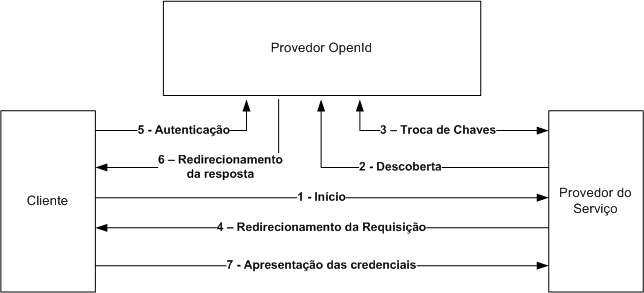
\includegraphics[width=0.8\textwidth]{openiddiagram.png}
\caption{Fluxo do protocolo OpenId, adaptado de~\cite{rfc6749}.}
\label{fig:openid}
\end{figure}

\begin{enumerate}[1 )]
\item  Início, Um cliente envia um indentificador OpenID que alega possuir.

\item  Descoberta, o Provedor do Serviço descobre o provedor OpenID correspondente ao identificador OpenID apresentado pelo cliente.

\item Troca de chaves,  segredos são trocadas entre o Provedor do Serviço e o Provedor OpenID.

\item O Provedor do Serviço redireciona o cliente para provedor de OpenID, para que ele possa se autenticar.

\item Autenticação, o cliente se autentica no provedor OpenID. (A maneira em que a autenticação ocorre está fora do escopo OpenID.)

\item O Provedor de OpenID redireciona novamente o Cliente para o Provedor do Serviço.

\item Apresentação das credenciais, finalmente, a carga OpenID contendo a declaração de identidade validada é enviada para o Provedor do Serviço.

\end{enumerate}

\subsection{SAML}

O \emph{Security Assertion Markup Language} - SAML é uma especificação padrão para troca de credenciais,\emph{tokens} de segurança, que contém informações de autenticação e autorização, baseadas em XML, que visam garantir a interoperabilidade entre diferentes sistemas. Foi desenvolvido em 2005 pela OASIS (OASIS,2005b; OASIS, 2005c). Ele está dividido no seguintes componentes: asserções, protocolos, ligações e perfis, que são descritos a seguir~\cite{Madsen2005}

Uma Asserção é um conjunto de informações que fornece uma ou mais informações feitas por uma autoridade SAML. Ela é dividida em três tipos diferentes: autenticação, atributo e decisão de autorização~\cite{Madsen2005,Nordbotten09,Bertino2010}. Uma asserção de autenticação, é aquela que afirma que determinada informação foi autenticada por um meio qualquer em determinado momento. Este tipo de asserção é geralmente emitido por uma autoridade SAML denominada de fornecedor de entidades. A sua responsabilidade é a de autenticar consumidor do serviço e manter registros dos dados relacionados com a sua sessão, enquanto esta for válida. O atributo é a asserção que contém informações específicas de um determinado cliente. E finalmente a decisão de autorização, que são as informação sobre a decisão de permitir, ou não, o acesso a um determinado recurso por parte do consumidor do serviço.

Os protocolos, nesse contexto são uma série de mensagens protocolares do tipo pedido/resposta que permitem um provedor de serviços, dentre outras coisas, solicitar a uma autoridade SAML, uma ou mais asserções, pedir a autenticação de um usuário a um provedor de identidades e obter as asserções correspondentes.

As ligações, que são aquelas que realizam o mapeamento entre mensagens protocolares e as normas de comunicação entre sistemas, em linhas gerais, define como mensagens SAML serão transportadas em cima dos protocolos padrão de mensagens e transporte.

Os perfis, são aqueles que definem um conjunto de restrições e ou extensões para o suporte da utilização de SAML em uma determinada aplicação.

Na versão 2.0 do SAML, foram adicionadas uma série de novos recursos tais como os pseudônimos, gerenciadores de identidades e de sessões, metadados, encriptação, perfis de atributos, suporte a dispositivos móveis, mecanismos que permitem a aplicação de políticas de privacidade e métodos de pesquisa de provedores de identidades.

\subsection{OAuth}

O \emph{Open Authorization Protocol - OAuth} é um protocolo desenvolvido com o objetivo de solucionar os problemas relacionados com a gestão de identidades entre provedores de serviços. A primeira versão 1.0 foi lançada em 2007, e sua última revisão foi publicada em 2010, sendo especificada no Request For Comments (RFC)5849~\cite{oauth210}. Em 2012, a versão 2.0 do protocolo, OAuth 2.0, foi lançada com objetivo de resolver problemas encontrados na versão 1.0, tais como escalabilidade e complexidade~\cite{rfc6749}.

Na última versão, 2.0, quatro papéis básicos são definidos e necessários para compreensão do fluxo de execução do protocolo, são eles: proprietário do recurso, que é a entidade que tem o poder de conceder a permissão de acesso, aos seus recursos, às outras entidades; O servidor de recursos, que é o responsável por hospedar e responder às solicitações de acesso a recursos protegidos, usando \emph{tokens} de acesso; Cliente, que é uma aplicação, que realiza solicitações de acesso de recursos protegidos, ao servidor de recursos, em nome do proprietário, dono do recurso, após a obtenção de sua autorização; E o servidor de autorização, que é responsável por emitir \emph{tokens} de acesso aos clientes, após autenticar e obter autorização do proprietário de recursos~\cite{rfc6749}.

%Na última versão, 2.0, quatro papéis básicos são definidos: proprietário do recurso, servidor de recursos, cliente e servidor de autorização~\cite{rfc6749}.

%O proprietário do recurso é a entidade que tem o poder de conceder a permissão de acesso, aos seus recursos, às outras entidades.

%O servidor de recursos é aquele responsável por hospedar os recursos protegidos, e tem a capacidade de responder às solicitações de acesso a recursos protegidos, usando \emph{tokens} de acesso.

%Já o cliente, é uma aplicação que realiza solicitações de acesso de recursos protegidos, ao servidor de recursos, em nome do proprietário dono do recurso após a obtenção da de sua  autorização.

%E por fim, o servidor de autorização, que é aquele que emite \emph{tokens} de acesso aos clientes, após autenticar e obter autorização do proprietário de recursos.

Na maioria dos casos, o papel do servidor de autorização e o servidor de recursos podem  ser representados por uma única entidade. A Figura~\ref{fig:diagramaoauth} apresenta de forma abstrata o fluxo do protocolo OAuth 2.0 e descreve a interação entre os quatro papéis.

\begin{figure}[!htb]
\centering
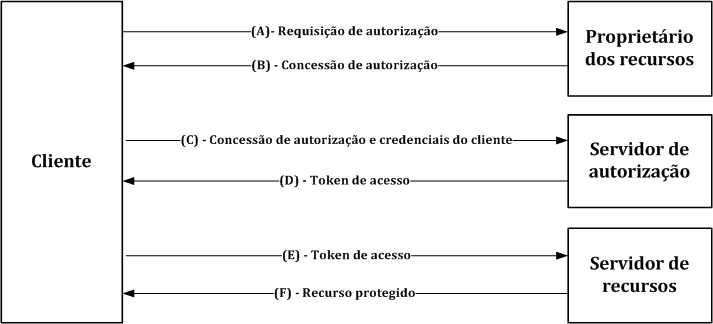
\includegraphics[width=0.8\textwidth]{diagrama_oauth2.png}
\caption{Fluxo do protocolo OAuth 2.0 adaptado de~\cite{rfc6749}.}
\label{fig:diagramaoauth}
\end{figure}

\begin{enumerate}[a )]
        \item O cliente solicita a autorização do proprietário do recurso.
        \item O cliente recebe uma concessão de autorização, que representa a autorização fornecida pelo proprietário do recurso.
        \item O cliente solicita ao servidor de autorização um \emph{token} de acesso que pode ser usado para acessar os recursos protegidos. Durante este processo, o cliente fornece suas credenciais e a concessão de autorização para autenticar-se com o servidor de autorização.
        \item O servidor de autorização confirma a validade das credenciais do cliente e da concessão de autorização, se elas forem válidas, ele então fornece ao cliente um \emph{token} de acesso.
        \item O cliente solicita os recursos protegidos, hospedados no servidor de recursos, apresentando o \emph{token} de acesso.
        \item  O proprietário do recurso verifica a validade do \emph{token} de acesso e, se válido, ele atende ao pedido.

\end{enumerate}

\subsection{Traust}

O sistema Traust é um serviço flexível de autorização voltado a sistemas abertos de larga escala. Ele utiliza sistemas de negociação de confiança para permitir que os clientes possam estabelecer uma confiança bilateral com provedores de recursos até então desconhecidos em tempo real, além de negociar o acesso a novos recursos em tempo de execução~\cite{traust08}.

Traust foi projetado para permitir sua integração direta com novas aplicações de reconhecimento de confiança ou indiretamente com aplicações legadas existentes. Essa flexibilidade abre o caminho para a adoção incremental de tecnologias de negociação de confiança sem a necessidade de atualizações de protocolo ou de software~\cite{traust08}.

Em síntese, o Traust atua como um intermediário que fornece tokens de segurança que permitem acesso aos recursos localizados em um determinado domínio de segurança. Os formatos dos tokens utilizados podem variar e ser de qualquer formato, incluindo usuário e senha, bilhetes Kerberos, afirmações SAML e ou certificados X.509~\cite{traust08}.

Dessa forma, ele pode ser integrado diretamente a aplicativos mais novos, que sejam baseados em confiança e que tenham por finalidade  prover a autorização a sistemas abertos.

\subsection{eXtensible Access Control Markup Language}
O \emph{eXtensible Access Control Markup Language} (XACML) foi proposto pelo grupo OASIS e atualmente está na versão 3.0~\cite{XACML}. O XACML é um padrão baseado em XML que define linguagens de marcação e possibilita especificar políticas de controle de acesso e um modelo de processamento para avaliar solicitações de autorização de acordo com as políticas definidas que são utilizadas para controlar acesso a conteúdos e informações protegidas.

O XACML descreve uma linguagem para políticas de controle de acesso e têm pontos de extensão padrão para definição de novas funções, tipos de dados e combinações lógicas o que o torna flexível e extensível.

Um dos diferenciais do XACML em relação a outros padrões proprietários é que é independente de uma implementação específica o que permite que ele possa ser utilizado tanto para prover controle de acesso a sistemas robustos bem como a um recurso específico. Outro ponto importante e que o XACML pode ser combinado ao SAML e assim possibilitar a criação de um sistema de autorização completo.

\section{Síntese do Capítulo}

Este capítulo apresentou conceitos básicos da arquitetura orientada a serviços. Foram abordados conceitos fundamentais da tecnologia Web Services, REST, sendo apresentadas as definições de sua estrutura. Além disso, foram descritos alguns protocolos de autenticação e autorização. No que tange a segurança em SOA, foram apresentados os conceitos básicos de segurança e elencadas algumas das principais vulnerabilidades que afetam a arquitetura orientada a serviços. No próximo capítulo, será descrito o protocolo de autenticação e autorização proposto e sua análise formal, utilizando para isso a lógica BAN.

  %---------- Segundo Capítulo ----------
\chapter{Mapeamento Sistemático}
\section{Introdução}
%A utilização da arquitetura orientada a serviços (SOA), que consiste em uma coleção de componentes distribuídos que fornecem e ou consomem serviços\cite{Clements2010}, tem sido amplamente utilizada por um grande número de empresas.

%Serviços correspondem a recursos de software bem definidos através de uma linguagem padrão, são auto-contidos,  proveem funcionalidades padrões do negócio, independentes do estado ou contexto de outros serviços \cite{Furtado2009}.

%Nesse contexto a utilização de serviços padronizados tornou-se a solução para a problemática da interoparibilidade entre sistemas, uma vez que permitiu a integração automatizada de negócios entre aplicações.

A utilização da SOA tornou-se uma solução para a problemática da interoperabilidade entre sistemas, uma vez que permitiu a integração automatizada de negócios entre aplicações. Contudo, apesar dos benefícios, existem vários desafios que devem ser considerados quando da implantação de uma arquitetura orientada a serviços~\cite{marks2006}. Dentre eles destaca-se o requisito não funcional de segurança, que deve ser muito bem planejado de forma que o serviço oferecido não seja vulnerável a ameaças que comprometam sua integridade, confidencialidade, disponibilidade e autenticidade. Dessa forma, é de suma importância conhecer e aplicar os mecanismos de segurança em uma Arquitetura Orientada a Serviços.

Com a intenção de identificar trabalhos primários relevantes e reconhecidos, com vistas a aumentar o conhecimento da aplicabilidade de mecanismos de segurança a arquitetura orientada a serviços, fez-se necessário realizar um mapeamento sistemático que identificasse as principais pesquisas que envolvessem o tema segurança em SOA.

%Dentre as alternativas optou-se pelo mapeamento sistemático que tem como finalidade, classificar e agregar à literatura estudos relevantes. Seu foco está na  pesquisa mais ampla e de natureza exploratória, cuja finalidade é fornecer uma visão geral e encontrar evidências de uma área de pesquisa.

\section{Mapeamento Sistemático}

Essa seção descreve os resultados do mapeamento sistemático conduzido, sendo estruturada conforme as diretrizes discutidas em~\cite{Petersen2008}.

%O mapeamento sistemático possibilita verificar e identificar evidências de uma área, por meio de uma revisão ampla de estudos primários \cite{guidelines-2007}. Já a revisão sistemática foca em questões de pesquisa bem definidas, mais específicas, que podem ser respondidas por pesquisa experimental\cite{Kitchenham2010}. A metodologia adotada para a organizar e estruturar este mapeamento seguiu as diretrizes prospostas em \cite{sbcars2013}.

\section{Protocolo de Estudo}

Para a realização do mapeamento sistemático foi definido um protocolo de estudo que contemplasse as questões de pesquisa, a string de busca e os critérios de exclusão e inclusão de artigos. A finalidade deste processo é a de documentar as etapas do mapeamento além de permitir a sua replicação por outros pesquisadores.

\section{Questões de Pesquisa (QP)}

Com a finalidade de identificar as principais contribuições e estudos sobre \ ``Segurança e SOA\ '' a pesquisa toma a vertente mais específica com as questões abaixo:

\begin{enumerate}[ QP1 )]

    \item Quais são os principais veículos que publicam artigos nessa área?
    busca-se verificar quais são os principais veículos que publicam informações sobre segurança em SOA, de forma que seja possível categorizar e verificar onde foram publicadas as contribuições mais significativas.
	
	\item Qual o tipo de contribuição é a mais proposta nas pesquisas realizadas?
    Neste caso, procura-se verificar quais são as principais contribuições de pesquisa, identificando se o tipo da contribuição é uma proposta, solução, avaliação, validação de algum estudo ou um artigo de opinião.


	\item Quais atributos de segurança são mais abordados nos estudos? Objetiva-se identificar dentre os atributos privacidade, confidencialidade, autenticidade e disponibilidade,  quais são os mais abordados nos estudos categorizados e classificados como solução. Além disso, quando uma solução não for classificada em nenhum desses atributos ele deverá ser classificado como qualidade de serviço. Neste caso, serão classificados os artigos que não se enquadrarem em nenhum dos atributos anteriores, mas que mesmo assim, vise garantir a qualidade de outros atributos que no contexto de segurança em SOA seja relevante. Por exemplo, desempenho e escalabilidade.

    \item Quais contribuições classificadas como solução e categorizadas como: método, técnica ou ferramenta/arquitetura, foram os mais propostos nas pesquisas? Objetiva-se identificar dentre os artigos selecionados e categorizados como Solução quais deles podem ser classificados e quantificados como método, técnica ou ferramenta/arquitetura.



\end{enumerate}

\section{Estratégia de Busca}\label{sec:Obj1}

É oportuno definir uma estratégia de busca para a pesquisa dos estudos primários, sendo necessário determinar as palavras chaves a serem pesquisadas e também onde as buscas serão realizadas~\cite{guidelines-2007}.
A estratégia de busca adotada consistiu objetivamente na busca eletrônica das seguintes bibliotecas digitais:
\begin{enumerate}[ a )]
    \item ACM Digital Library referente aos seguintes periódicos:
       \begin{enumerate}
            \item ACM Transactions on Information and System Security (TISSEC);
            \item ACM Computing Surveys (CSUR).
       \end{enumerate}

    \item IEEE Xplore, apenas por periódicos e
    \item DBLP Computer Science Bibliography nas seguintes conferências:
      \begin{enumerate}
            \item ICWS International Conference on Web Services;
            \item SERVICES;
            \item ARES.
      \end{enumerate}

\end{enumerate}

A opção por essas fontes foi motivada por uma pesquisa inicial realizada na base de dados da DBLP, que retornou 77 publicações. Sendo que após uma análise preliminar, observou-se que as conferências mais relevantes quantitativamente foram as citadas no item c desta seção. Seguiu-se o mesmo procedimento para as bibliotecas citadas nos ítens a e b.

No contexto da elaboração dos termos de busca, para  a base de dados eletrônica, usou-se a abordagem descrita em~\cite{guidelines-2007}, que consiste em criar os termos de busca a partir de questões de pesquisa, usando a composição de operadores AND e OR. Dessa forma, a \emph{string} de busca usada na realização desse estudo foi \textbf{\emph{SOA and SECURITY}} não sendo usados sinônimos ou outras variações.

\section{Critérios de Inclusão e Exclusão}

Após serem realizadas as pesquisas, de acordo com a \emph{string} de busca,  vários estudos primários foram recuperados e avaliados  de forma que fossem  excluídos aqueles que não satisfizessem os objetivos do estudo. A investigação dos estudos consistiu inicialmente em analisar o título, o resumo, a introdução e a conclusão.

As conclusões foram analisadas para entender melhor as contribuições do trabalho. Os critérios de seleção dos estudos foram baseados nas questões de pesquisa e todos os estudos recuperados foram armazenados. Logo, para este mapeamento foram definidos os seguintes critérios de inclusão e exclusão:
\begin{itemize}
\item No que se refere aos critérios de inclusão, foram incluídos todos os artigos que faziam referência a SOA Security e que foram publicados nos periódicos e conferências publicados no período compreendido do ano de 2000 até 2013 e que satisfizessem a \emph{string} de busca anteriormente definida.

\item No que tange os critérios de exclusão, foram excluídos os artigos e resumos com menos de quatro páginas, artigos que não tratavam diretamente do tema SOA \emph{SECURITY}, contribuições que, apesar de versar sobre SOA, não faziam referência à segurança e vice-versa, as que tratavam de segurança, mais não tratavam de arquitetura orientada a serviços. Além disso, foram também excluídos os estudos irrelevantes para a pesquisa e aqueles que não puderam ser obtidos gratuitamente.
\end{itemize}

%\begin{itemize}
    %\item Critérios de Inclusão
      % \begin{enumerate}
       %     \item Foram incluídos todos os artigos que faziam referência a SOA Security e que foram publicados nos periódicos  e conferências   que satisfizessem a string de busca anteriormente definida;
      %      \item Estudos publicados no período compreendido do ano de 2000 até 2013.
       %\end{enumerate}

    % \item Critérios de Exclusão
      %\begin{enumerate}
       %     \item Artigos e resumos com menos de quatro páginas, estudos incompletos e repetidos e apresentações (Power Point);
      %      \item Artigos que não tratavam diretamente do tema SOA SECURITY;
        %    \item Contribuições que, apesar de versar sobre SOA, não faziam referência a segurança e vice-versa, as que tratavam de segurança, mais não tratavam de arquitetura orientada a serviços;
          %  \item Estudos irrelevantes para a pesquisa e aqueles que não puderam ser obtidos pela UNB.

     % \end{enumerate}

%\end{itemize}

\section{Coleta, Armazenamento dos Dados e Análise}

Após a seleção preliminar e seguindo o que foi preconizado na estratégia de busca, foram realizadas buscas automáticas a cada uma das bibliotecas digitais citadas na Seção~\ref{sec:Obj1}, sendo recuperadas ao todo 54 publicações. A última etapa da seleção consistiu em aplicar os critérios de exclusão e inclusão aos artigos selecionados, de forma que se obteve um total de 25 publicações, que foram analisadas e classificadas de acordo com a seguinte classificação:

\begin{enumerate}
            \item Veículos: Neste tópico buscou-se categorizar quais veículos que mais apresentaram publicações;
            \item Pesquisa: Este tópico foi utilizado para definir quais tipos de pesquisa foram propostas no estudo de forma que as publicações foram classificadas como:
                \begin{enumerate}[ a )]
                 \item Solução: Representa as publicações que propõem uma nova técnica, método ou ferramenta/arquitetura e que a partir dela possa ser realizado algum tipo de verificação de viabilidade;

                 \item Validação: Neste caso são proposições de validação de algum estudo que apresente rigor cientifico, tais como estudos empíricos ou provas da aplicação de alguma técnica, podendo ser uma validação formal ou experimental;

                 \item Avaliação: Publicações que apresentaram avaliações comparativas entre técnicas propostas de algum estudo relacionado a Segurança em SOA, sendo  classificado como:

                    \begin{itemize}
                         \item Avaliação Formal, que é aquele que possui detalhes do estudo, sendo possível, caso necessário, realizar uma reprodução do trabalho;

                        \item Avaliação Informal, que é  aquela em que os detalhes do estudo são poucos o que torna difícil sua reprodução;

                        \item Avaliação Preliminar, neste caso serão considerados os estudos cujos resultados podem ser questionados e não apresentam detalhes para reprodução.
                    \end{itemize}


                 \item Artigos de Opinião: que são estudos informais que fazem uma abordagem geral dos aspectos do tema Segurança em SOA.

            \end{enumerate}

            \item Contexto: Busca-se neste tópico classificar as publicações que sejam classificados como uma Solução e possuam atributos  relacionados a segurança em SOA que abordem: privacidade, confidencialidade, autenticidade e disponibilidade.

\end{enumerate}

\section{Resultados}
Nesta seção são descritos os resultados obtidos após o estudo e o mapeamento das principais publicações coletadas na seção 2.5 e que serão utilizados para responder as questões de pesquisas anteriormente definidas.

\subsection{QP 1 \- Questão de Pesquisa 1}

Quais são os principais veículos que publicam artigos nessa área?
Para responder essa pergunta foram analisados os 25 artigos selecionados após a aplicação dos critérios de exclusão e inclusão. Eles foram classificados de acordo com o veículo de publicação do artigo. Essa classificação é apresentada na figura~\ref{fig:grafico_qtd_veiculo}.

\begin{figure}[!htb]
\centering
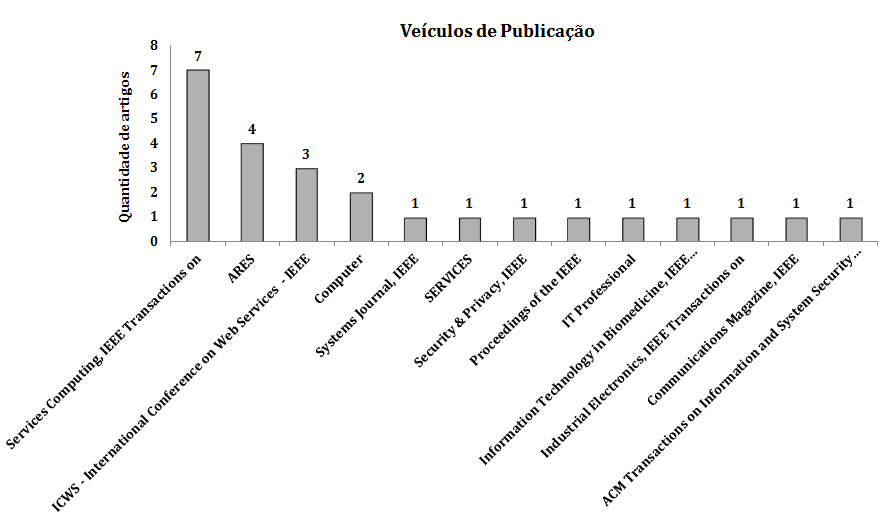
\includegraphics[scale=0.7]{qtd_veiculo_publicacao.png}
\caption{Gráfico representativo da quantidade de contribuições por veículo de publicação.}
\label{fig:grafico_qtd_veiculo}
\end{figure}

Verifica-se que os veículos que mais publicaram artigos relacionados a segurança em SOA foram Services Computing, ARES, ICWS e Computer com 28\%, 16\%, 12\% e 8\% dos artigos publicados, respectivamente. Eles reponderam juntos por aproximadamente 64\% das publicações.

\subsection{QP 2 \- Questão de Pesquisa 2}

Qual o tipo de contribuição é a mais proposta nas pesquisas realizadas?
Após a realização do mapeamento foi possível verificar que dentre os artigos mapeados houve artigos que fizeram referência a mais de um tipo de contribuição. Isso pode ser verificado no artigo proposto por~\cite{Delegation_Solution2011} que foi classificado como sendo uma Solução e uma Validação. Um outro exemplo pode ser observado no artigo~\cite{Vulnerability_Analysis2011} que foi classificado como sendo uma Solução e uma Avaliação. Dessa forma, a contribuição mais proposta foi a Solução com 42\% do total de artigos selecionados, seguidos por Avaliações e Artigos de Opinião ambos com 24\% e finalmente a Validação com 10\%. Dentre essas soluções, cabe ressaltar a que é proposta por~\cite{Vulnerability_Analysis2011}, que propõe um novo método denominado ATLIST, que realiza análise de vulnerabilidades em processos de negócios e serviços baseados em SOA. Este trabalho pode ser útil para a arquitetura de referência que será proposta como resultado deste trabalho de mestrado.

Além desta, outra que também deve ser citada é a que é idealizada por~\cite{Ontology2012}, neste artigo é proposta uma Ontologia, ASSERT4SOA, que foca na interoperabilidade e comparação de certificados heterogêneos e possibilitando a verificação em tempo de execução da conformidade dos serviços com os requisitos de segurança.

Outro artigo relevante para a problemática discutida nesta dissertação é o artigo proposto por~\cite{WeberAM07}. Nesta solução, é proposta uma ferramenta que tem por objetivo identificar possíveis violações de segurança em ambientes SOA. Na ferramenta são descritas formas para inspecionar os arquivos de configuração da plataforma SOA, sendo possível detectar possíveis violações de segurança. Sendo também realizada uma avaliação informal que procura analisar as melhores práticas de segurança em SOA.

Já quanto à contribuição que se refere à avaliação pode-se verificar 4 (quatro) artigos classificados neste tipo, são de avaliações formais, ou seja, estudos que traziam resultados detalhados que podem ser reproduzidos por outros pesquisadores. Um exemplo de avaliação formal pode ser identificado no artigo~\cite{Coetzee2012}. Este artigo analisa os desafios de segurança enfrentados em arquiteturas orientadas a serviço. Os autores propõe uma estrutura de segurança aplicada a SOA baseado em componentes, que consistem em uma variedade de controles que podem minimizar os desafios referentes à aplicação dos mecanismos de segurança em SOA. Os outros artigos classificados como avaliação foram classificados como avaliações informais 4 (quatro) artigos e experimentais 1 (um) artigo totalizando 5 (cinco) artigos.

No que se refere ao tipo de contribuição Validação, foram identificados 4(quatro) artigos  sendo 3(três) validações formais e 1(uma) experimental. Neste tipo de contribuição é relevante citar o trabalho realizado no artigo~\cite{CrossRealmSOA2012}. Neste artigo, é proposta uma ferramenta, que também é uma solução técnica, de um novo protocolo de autenticação para interações de serviços dinâmicos, com base na noção de sessões de negócios multipartidárias orientadas a serviços. Esse protocolo não requer conversão de credencial nem estabelecimento de qualquer caminho de autenticação entre os serviços que participam de uma sessão de negócios. No protocolo são realizadas provas e experimentos para verificar a viabilidade da nova técnica. Este trabalho também poderá ser útil para a arquitetura de referência que será proposta, uma vez que traz uma nova técnica que pode ser utilizada como referência nos processos de autenticação dos serviços oferecidos.

E por fim, no caso dos Artigos de Opinião, foram verificados 9(nove) artigos que faziam uma abordagem geral dos panoramas e desafios de segurança em arquitetura orientada a serviços. Nesses artigos não foi proposto nenhuma contribuição relevante. Porém, como eles se enquadraram nos critérios de busca estabelecidos, foram considerados.

A figura~\ref{fig:Tipo_Contribuicao} apresenta os resultados categorizados pelo tipo da contribuição sendo apresentado o quantitativo de publicações.

\begin{figure}[!htb]
\centering
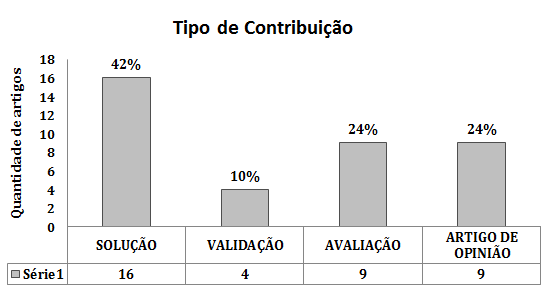
\includegraphics[width=0.8\textwidth]{tipo_contribuicao_3.png}
\caption{Gráfico representativo dos tipos de contribuições}
\label{fig:Tipo_Contribuicao}
\end{figure}


\subsection{QP 3 \- Questão de Pesquisa 3}

Quais atributos de segurança são os mais abordados nos estudos?
Para responder essa pergunta inicialmente realizou-se uma análise nos artigos classificados como Solução. Em seguida foram categorizados de acordo com os atributos relativos à segurança em ambiente SOA. Os atributos analisados foram: integridade, autenticidade, disponibilidade e confidencialidade. Foi possível verificar que dentre os artigos mapeados houve artigos que faziam referência a mais de um atributo. Um exemplo desse fato é descrito na publicação de~\cite{pattern-driven2008} onde são abordados todos os atributos de segurança: integridade, autenticidade, disponibilidade e confidencialidade. Dessa forma, o número de artigos mapeados com os atributos descritos não será equivalente com o número de artigos totalizados no mapeamento.

Sendo assim, o mapeamento identificou que os conceitos mais abordados referem-se aos atributos de autenticidade com 32\% ou 13 artigos e Integridade com 28\% ou 11 artigos. Já o atributo confidencialidade foi verificado em 20\% das publicações, com 8 artigos, e o atributo disponibilidade foi verificado em 15\% das publicações, sendo identificado em 6 artigos. Finalmente, para os artigos que foram classificados como uma solução e que não se enquadraram em nenhum dos atributos, sendo classificados como atributos de qualidade de serviços, foram identificados em apenas 5\% das publicações ou 2 artigos. A Figura~\ref{fig:TipoConceito} apresenta graficamente essa categorização.

\begin{figure}[!htb]
\centering
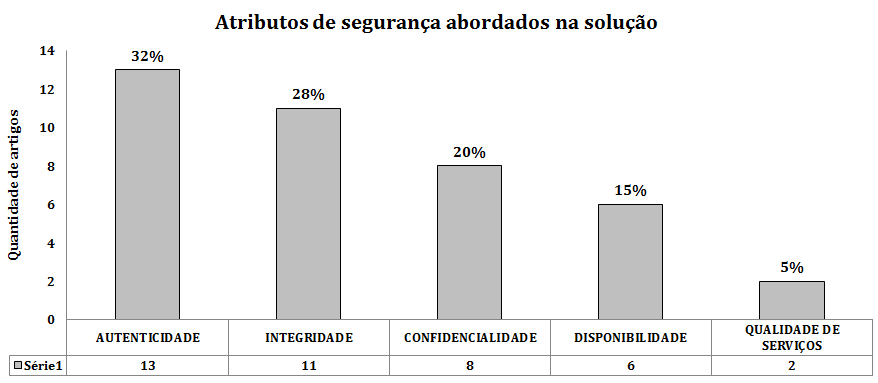
\includegraphics[width=1.0\textwidth]{Atributo_Seguranca_Solucao.png}
\caption{Gráfico dos atributos de segurança abordados na solução}
\label{fig:TipoConceito}
\end{figure}

\subsection{QP 4 \- Questão de Pesquisa 4}

Quais contribuições classificadas como solução e categorizadas como: método, técnica ou ferramenta/arquitetura, foram os mais propostos nas pesquisas?
Para responder essa pergunta, foi realizada uma análise dos artigos classificados como solução. Em seguida foram categorizados de acordo com os tipos: técnica, método ou ferramenta/arquitetura. Verificou-se que entre os artigos mapeados um artigo que fez referência a mais de um tipo de solução.  Esse artigo é descrito na publicação de~\cite{CrossRealmSOA2012} onde são abordados os tipos de solução técnica e ferramenta/arquitetura. Dessa forma, o número de artigos mapeados como sendo uma solução do tipo: método, técnica ou ferramenta/arquitetura não será equivalente com o número de artigos totalizados no mapeamento.

O mapeamento identificou dentre as contribuições classificadas como solução, que o tipo de solução mais proposta é a de solução técnica com 44\% das contribuições ou 7 artigos. As classificadas como ferramenta/arquitetura, foi observado em 31\% das contribuições, ou 5 artigos. Finalmente, o tipo de solução classificado como método, foi verificado em 25\% das contribuições selecionadas, ou 4 artigos. A figura~\ref{fig:TipoConceito} apresenta graficamente essa categorização.


\begin{figure}[!htb]
\centering
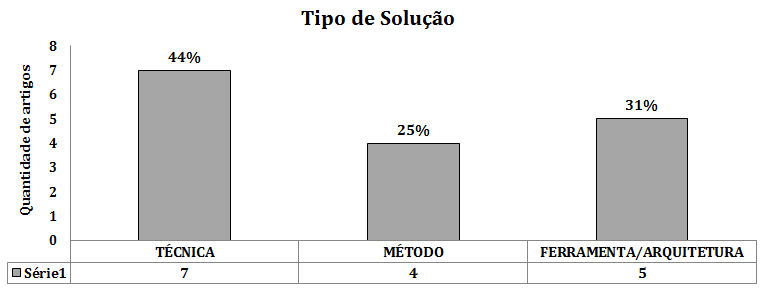
\includegraphics[width=1.0\textwidth]{tipo_solucao.png}
\caption{Gráfico dos tipos de Solução mais propostos}
\label{fig:tipo_solucao}
\end{figure}
%---------- Segundo Capitulo ----------
\subsection{Discussão sobre os Resultados}

De acordo com os resultados obtidos por este mapeamento sistemático foi possível observar que a maioria dos artigos se concentram nos veículos: Services Computing, ARES, ICWS e Computer com 28\%, 16\%, 12\% e 8\%, respectivamente. Eles reponderam juntos por aproximadamente 64\% das publicações.

No que tange os resultados obtidos a respeito do tipo de contribuições, verificou-se que a maior parte de contribuições foram de soluções com 42\% dos artigos e que destas destacaram-se as soluções técnicas com 44\% dos artigos classificados nesta faceta de pesquisa. Este resultado denota que os pesquisadores tem buscado estabelecer padrões e procedimentos  com objetivos específicos de resolver problemas ou melhorar as técnicas existentes que estejam  relacionados a segurança em SOA.

No contexto das contribuições referentes aos atributos de segurança que foram abordados e classificados com solução, verificou-se que as maiores preocupações estavam associadas aos atributos de  autenticidade, integridade e confidencialidade com 33\%, 27\% e 20\% das contribuições respectivamente. Dessa forma, verifica-se que dentre as soluções anteriormente citadas a maior preocupação é em estabelecer técnicas eficientes para autenticar os serviços e garantir que o conteúdo das mensagens não seja modificado. Isso pode denotar uma preocupação com o desempenho dos serviços no momento da aplicação dos mecanismos de segurança.
%
%\subsection{Ameaças a validade}

%As possíveis ameaças aos resultados dessa pesquisa são caracterizados a seguir e seguem  a classificação proposta por \cite{ leedy1980practical} e que foram estruturadas no artigo \cite{sbcars2013}.

\section{Síntese do Capítulo}

O mapeamento sistemático realizado, possibilitou aprofundar os conhecimentos referentes à segurança em SOA. Sendo possível verificar quais são os principais veículos que publicam artigos nesta área, o que ajuda a direcionar os estudos. Também foi possível identificar e analisar quais são os tipos de contribuições que mais são propostas nas pesquisas envolvendo esta temática. Além disso, verificou-se dentre as contribuições propostas como solução, quais delas envolviam atributos de segurança e que tratavam de integridade, autenticidade, disponibilidade e confidencialidade. E por fim, nas contribuições classificadas como solução, foi possível identificar e quantificar quais tipos de solução (método, técnica e ferramentas/arquitetura) foram as mais propostas.

Com este mapeamento sistemático foi possível identificar alguns artigos que serão fundamentais para nortear a pesquisa desenvolvida nesta dissertação. Eles são descritos a seguir:

No artigo~\cite{WeberAM07}, são descritas formas para inspecionar os arquivos de configuração da plataforma SOA, sendo possível detectar possíveis violações de segurança. Um dos focos do trabalho está relacionado com as melhores práticas para a implantação de segurança em SOA, o que pode enriquecer a arquitetura de referência proposta nesta dissertação.

Outro trabalho que também deve ser citado é a publicação~\cite{pattern-driven2008} onde são abordados todos os atributos de segurança: integridade, autenticidade, disponibilidade e confidencialidade. Neste trabalho é proposto uma nova abordagem para proteger aplicativos de SOA. Outro ponto importante, e que a segurança não é considerada como um aspecto isolado, mas como um aspecto presente em todas as fases de um desenvolvimento do sistema.

O artigo~\cite{Coetzee2012} analisa os desafios de segurança enfrentados em arquiteturas orientadas a serviço. Sendo proposta uma estrutura de segurança aplicada a SOA, baseado em componentes, que consiste em uma variedade de controles que podem minimizar os desafios referentes à aplicação dos mecanismos de segurança em SOA. Esse artigo realça os desafios de segurança em SOA e pode servir como base para a proposta de criação da arquitetura de referência. 
    %\chapter{Protocolo de Autenticação e Autorização proposto}\label{cap:Protocolo}
\section{Introdução}
%A Polícia Civil do Distrito Federal, diante da necessidade de compartilhar suas informações com órgão parceiros, no intuito de possibilitar que os sistemas possam ser integrados de forma eficiente e principalmente segura busca estabelecer uma arquitetura de referência para a adoção de uma arquitetura orientada a serviços. Essa arquitetura deve primar pela segurança, haja vista a criticidade e sensibilidade das informações que são tratadas no âmbito da PCDF.

%Dessa forma, optou-se por adotar a tecnologia de Web Services usando o protocolo REST para implementar SOA na instituição. Neste caso, estudos específicos foram realizados com vistas a estabelecer uma política de segurança eficiente que possibilite o fornecimento dos serviços e promova a integração com os órgãos parceiros.
A Polícia Civil do Distrito Federal, diante da necessidade de compartilhar suas informações com órgão parceiros, no intuito de possibilitar que os sistemas possam ser integrados de forma eficiente e principalmente segura busca estabelecer uma arquitetura de referência para a adoção de uma arquitetura orientada a serviços. Essa arquitetura deve primar pela segurança, haja vista a criticidade e sensibilidade das informações que são tratadas no âmbito da PCDF.

Dessa forma, optou-se por adotar a Web services \emph{RESTFull} para implementar SOA na Instituição. Neste caso, estudos específicos foram realizados com vistas a estabelecer uma política de segurança eficiente que possibilite o fornecimento dos serviços e promova a integração com os órgãos parceiros. Sendo assim, surgiu a necessidade da criação de um protocolo seguro e personalizado de autenticação e autorização que atenda às necessidades da PCDF.

\section{Requisitos do Protocolo}\label{sec:reqprotocolo}

O protocolo de autenticação e autorização proposto deverá ser aderente a arquitetura REST, de forma que possa permitir que os serviços ofertados pela Divisão de Tecnologia possam ser acessados por um número relativamente grande de clientes. Os requisitos inerentes ao protocolo são descritos nesta seção.

\begin{enumerate}[RQ1]

\item Para promover a segurança de sessão, toda comunicação entre o cliente e o servidor será realizada utilizando HTTPS \emph{(Hypertext Transfer Protocol over Secure Sockets Layer)}, usando o SSL/TLS para garantir a confidencialidade e integridade para a sessão. Para isso será usado o certificado digital X.509, emitido por uma autoridade de certificação, para encriptar as comunicações e garantir a autenticidade do servidor e do cliente. Devendo os clientes realizar a validação do certificado antes de interagir com o servidor.

\item Será utilizado a criptografia assimétrica para promover a segurança na troca de mensagens realizada entre o Cliente e a PCDF. Todas as mensagens deverão ser assinadas digitalmente. Para isso, será utilizado uma função hash, com o algoritmo SHA(Secure Hash Algorithm).

\item O protocolo deverá permitir acesso aos serviços apenas ao pessoal autorizado, de forma que a autenticação e autorização, siga padrões definidos na política de segurança. Sendo que para ser autenticado e autorizado o usuário deverá apresentar credenciais válidas. Essas credenciais deverão ser criptografadas, assinadas e enviadas no cabeçalho do protocolo HTTPS. Devendo ser escalável em termos de sobrecarga, tamanho do domínio de proteção e de manutenção. Além disso, ele deverá permitir a preservação de privacidade, uma vez que para proteger os clientes e fornecedores de recursos de entidades maliciosas, suas interações deverão revelar o mínimo de informações possíveis.

\item A autenticação e autorização será baseada em desafios e resposta, que serão elaborados a partir da apresentação de declarações de identidade (Claims). Tal requisito torna mais flexível o gerenciamento da identidade do usuário, uma vez que possibilita ao administrador desabilitar credenciais que tenham sido comprometidas de forma transparente ao usuário.

\item A política de autenticação e autorização proposta no protocolo será estabelecida por meio de contrato onde serão definidos todas as regras que deverão ser atendidas pelos usuário e pelo fornecedor do serviço.

    Dessa forma, para que qualquer usuário possa ter acesso aos serviços ofertados pela Divisão de Tecnologia da PCDF ele deverá concordar com um contrato prévio de acesso. Devendo primeiramente ser cadastrado e ter definido quais são seus privilégios de acesso/autorização. Uma vez cadastrado o usuário deverá informar os dados que possam comprovar sua identidade no momento da autenticação de forma que ele possa ser autorizado de acordo com o seus privilégios.

    No momento do credenciamento será gerado para o cliente múltiplas credenciais, que serão utilizadas no processo de autenticação e autorização, essas informações serão compartilhados entre o Cliente o Servidor de Autenticação e Autorização e o Servidor REST. Além disso, o Contrato poderá ter acesso a múltiplos serviços. A Figura ~\ref{fig:diagrama_relacionamento} apresenta o relacionamento entre o contrato, credenciais e serviços.

\begin{figure}[!htb]
    \centering
    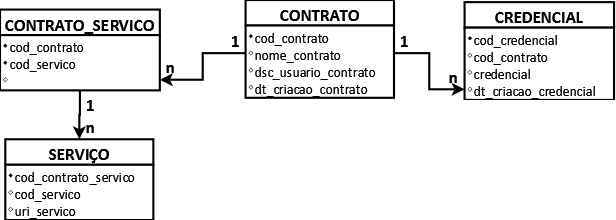
\includegraphics[width=0.8\textwidth]{modelo_relacionamento_contrato1.png}
    \caption{Diagrama de relacionamento entre contrato, credenciais e usuários}
    \label{fig:diagrama_relacionamento}
\end{figure}

\end{enumerate}


%Para a implementação de segurança em aplicações REST, verificou-se que ela passa basicamente pela aplicação de segurança em protocolos \emph{HTTP}, que oferece dois tipos de autenticação:  \emph{Basic} e \emph{Digest}.

%A autenticação Basic é um modelo baseado no desafio e resposta, sendo utilizada por servidores HTTP para validar a autenticação~\cite{franks1999}. Desta forma, quando o cliente tenta acessar algum recurso protegido, a sua identidade é requerida pelo servidor, o cliente então fornece a resposta codificada em base64 no header \emph{HTTP},  se a resposta for correta ela terá acesso ao sistema. Porém, por não criptografar o desafio, estando esse apenas codificado, faz com que ele seja vulnerável e sujeito a ataques, como por exemplo, os de repetição.

%Já na Digest, o processo é o mesmo que na autenticação básica. Sendo que seu mecanismo de autenticação é um pouco mais complexo, uma vez que ele gera um HASH, geralmente utilizando o algoritmo MD5, do desafio que será enviado pelo servidor ao cliente ~\cite{franks1999}. Apesar de ser mais seguro do que a autenticação básica, autenticação HTTP Digest também é vulnerável à ataques, como por exemplo o man-in-the-middle.  Para evitar esse problema, deve ser empregado a segurança na camada de transporte~\cite{Webber10}.

\section{Arquitetura do Protoloco}\label{sec:ArqProtocolo}

A arquitetura do protocolo proposto é apresentada na Figura~\ref{fig:arquiteturaprotocolo}. O protocolo é composto por quatro componentes: Cliente, Servidor de Autenticação e Autorização, Servidor REST, e Banco de Dados de Autenticação e Autorização.

\begin{figure}[!htb]
    \centering
    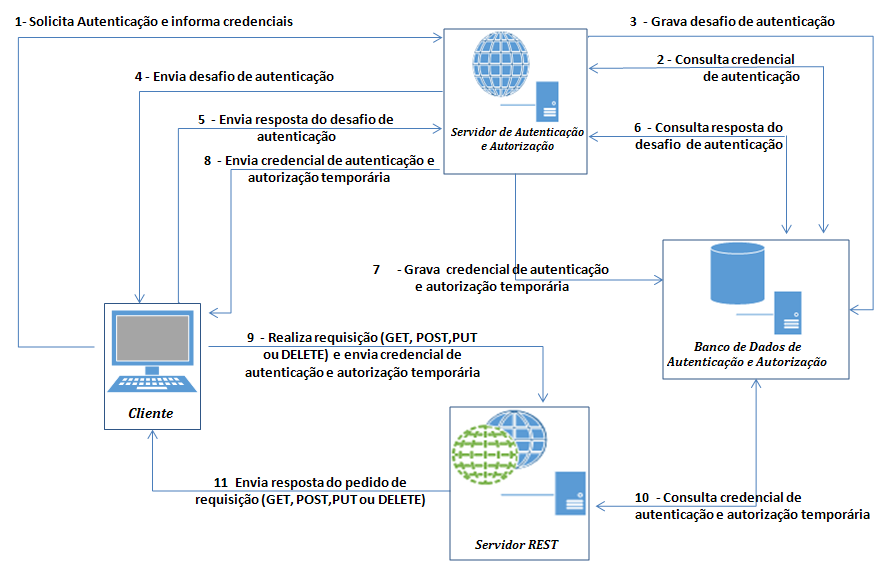
\includegraphics[width=0.8\textwidth]{arquitetura_protocolo.png}
    \caption{Fluxo do protocolo de autenticação/autorização proposto, 1º cenário.}
    \label{fig:arquiteturaprotocolo}
\end{figure}

Os componentes da arquitetura são detalhados a seguir.

Cliente: O componente Cliente na arquitetura do protocolo representa as Instituições ou Órgãos conveniados, que após firmar um contrato, podem consumir os serviços ofertados pela PCDF.

Servidor de Autenticação e Autorização: Este componente tem um papel fundamental na arquitetura do protocolo, pois é nele que o gerenciamento de autenticação e autorização é realizado. Desta forma, o servidor de Autenticação e Autorização é responsável por realizar os processos de verificação e validação de credenciais, criação dos desafios de autenticação, criação de \emph{tokens} JSON e a criação e o gerenciamento das credenciais de autenticação e autorização temporárias, que são utilizados pelos clientes para consumir os serviços requisitados.

Servidor REST: Esse é um servidor de fachada que abstrai toda lógica necessária para o consumo dos serviços.Neste servidor estão concentrados os serviços REST disponibilizados pela PCDF. Desta forma, quando um Cliente necessita acessar um serviço, primeiramente ele deve ser autenticado e autorizado no servidor de Autenticação e Autorização. Após esse processo, o Cliente faz a requisição ao servidor de REST, que realiza as verificações necessárias para saber se o Cliente tem privilégios ou não para acessar o serviço. Ele acessa a base de dados de Autenticação e Autorização para confirmar as credenciais de autenticação e autorização temporária informadas e caso elas sejam válidas ele permite que o Cliente acesse o serviço requerido. Um ponto importante a ser destacado é que os desenvolvedores, ao desenvolver um serviço, não necessitam ter preocupações de segurança, uma vez que é esse componente que realiza esse atividade.

Banco de Autenticação e Autorização: Servidor de banco de dados que contém a estrutura de banco de dados necessário  para o funcionamento dos serviços de autenticação e autorização. É neste servidor que são gravados as credenciais, usuários, os desafios e as credenciais de autorização e autenticação temporária.


\subsection{Visão geral do protocolo de Autenticação e Autorização proposto}

Para ter acesso a API \emph{REST}, referente aos serviços ofertados, o cliente deverá ser autenticado e autorizado a acessar o serviço. Para isso, será usado a autenticação baseada em \emph{tokens} de segurança, que são recipientes de reivindicações da autoridade emissora. Os \emph{tokens} de segurança utilizados serão os \emph{Web Tokens} no formato \emph{JSON}. Esse, ao contrário dos tokens \emph{SAML}, que são baseados em \emph{XML}, são mais compactos e, portanto mais adequados para serem usados em um cabeçalho \emph{HTTP}. Além disso, todas as mensagens deverão ser assinadas e criptografadas de forma assimétrica. O processo de autenticação e autorização é descrito em dois cenários distintos. No primeiro cenário, representado na figura ~\ref{fig:protocoloseguro}, o Cliente, não está autenticado. No segundo cenário, ele está autenticado e possui uma credencial de autorização. %Esse último é representado na figura ~\ref{fig:cenario2}.

\subsubsection{Primeiro cenário}
No primeiro cenário, o cliente não está autenticado, e irá solicitar a autenticação pela primeira vez, conforme descrito a seguir:
\newline
\begin{figure}[!htb]
    \centering
    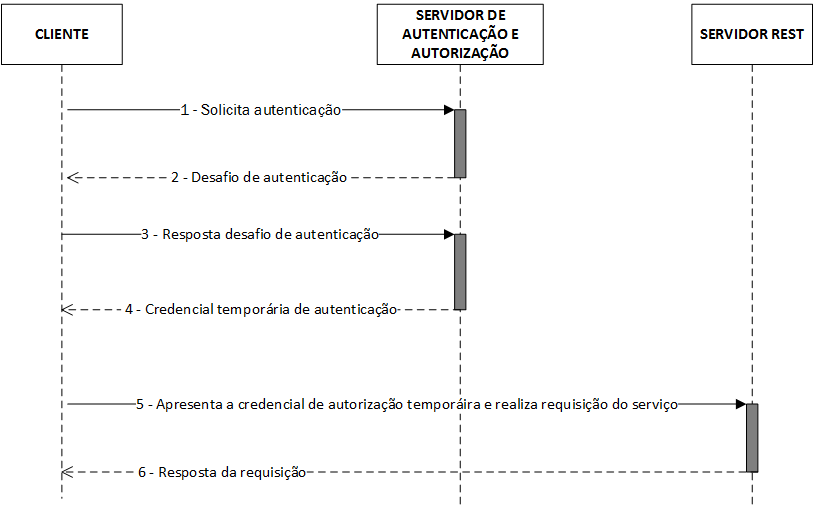
\includegraphics[width=1.0\textwidth]{fluxo_autenticacao.png}
    \caption{Fluxo do protocolo de autenticação/autorização proposto, 1º cenário.}
    \label{fig:protocoloseguro}
\end{figure}


O protocolo tem início quando o Cliente envia uma solicitação de autenticação ao servidor de Autenticação e Autorização. Esse pedido é realizado por meio de uma mensagem (mensagem 1 da Figura~\ref{fig:protocoloseguro}) que contém um \emph{token} JSON, enviado no cabeçalho HTTP da requisição REST. O \emph{token} contém uma credencial, extraída de forma aleatória da tabela de credenciais do Cliente. O token é assinado digitalmente pelo Cliente e cifrado com a chave pública do servidor de Autenticação e Autorização. É importante frisar que tanto o Cliente quanto o servidor de Autenticação e Autorização possuem as mesmas tabelas de credenciais e de serviços, pois elas são geradas no momento de assinatura do contrato de prestação do serviço.

Na segunda mensagem, ao receber uma solicitação de autenticação, o servidor de Autenticação e Autorização extrai o token cifrado com sua chave privada e verifica a autenticidade e integridade da requisição por meio da verificação da assinatura digital do Cliente.  Se houver qualquer problema, uma mensagem de erro HTTP (código 401): usuário não autorizado, é retornada ao Cliente.
Outra verificação que é realizada é a do \emph{timestamp}, que se refere ao tempo de envio da mensagem, se ela tiver sido enviada em um período de tempo superior ao pré-estabelecido no contrato, o Cliente também recebe uma mensagem de erro HTTP de usuário não autenticado.

Caso não haja problemas, procede-se com o processo de validação da credencial informada, que consiste em consultar a credencial em uma base de dados e se a credencial for válida e estiver associada ao Cliente, o Servidor de Autenticação e Autorização gera um desafio de autenticação. Tal desafio consiste em fazer uma busca aleatória à tabela de credenciais e selecionar um código de credencial que esteja associado ao Cliente. Em seguida grava-se o desafio, a data e hora de geração do desafio e a resposta que o Cliente deverá fornecer. um \emph{token} JSON, contendo o código do desafio, o código da credencial e um \emph{timestamp} representando a data e hora de criação do desafio, é enviado ao Cliente, assinado digitalmente pelo servidor de Autenticação e Autorização e cifrado com a chave pública do Cliente que está solicitando a autenticação.

Na terceira mensagem, após receber o desafio do servidor de Autenticação e Autorização, o Cliente, extrai o token cifrado com sua chave privada e verifica a autenticidade e integridade da requisição por meio da verificação da assinatura digital do servidor de Autenticação e Autorização. Em seguida verifica o \emph{timestamp}, cujo objetivo é o de verificar se a mensagem foi enviada em um período de tempo superior ao pré-estabelecido no contrato. Se houver qualquer problema, o processo de autenticação atual é descartado e inicia-se um novo processo de autenticação.

Caso não haja problemas, o Cliente verifica e responde o desafio solicitado, enviando-o, juntamente com um \emph{timestamp} e o código do serviço, que ele deseja consumir, para o Servidor de Autenticação e Autorização por meio de um \emph{token} JSON, que é assinado digitalmente pelo Cliente e cifrado com a chave pública do servidor de Autenticação e Autorização.

Na quarta mensagem, o servidor de Autenticação e Autorização recebe a resposta do desafio de autenticação, decifra o token e verifica a autenticidade e integridade da requisição por meio da verificação da assinatura digital do Cliente.  Não ocorrendo problemas, inicia-se o processo de verificação da resposta. A primeira verificação que é realizada refere-se ao tempo de geração do desafio, por meio do \emph{timestamp}. Se a resposta tiver sido enviada em um período de tempo superior ao pré-estabelecido em contrato, o servidor de Autenticação e Autorização envia uma mensagem de erro HTTP (código 401): usuário não autorizado, ao Cliente. Caso contrário, ele procede com a verificação do desafio que consiste em realizar uma consulta na tabela de desafios verificando se a resposta dada é a mesma que a esperada. Caso a resposta esteja correta o servidor de Autenticação e Autorização autentica o Cliente. Em seguida ele verifica, pelo código do serviço requisitado se o Cliente tem privilégios necessários para consumir o serviço requisitado.

Se a resposta for positiva, o servidor de Autenticação e Autorização gera uma credencial de autenticação e autorização temporária para o serviço solicitado. Ela é gravada em uma tabela de credencias de autorização temporária juntamente com a data e hora de criação, data de expiração e o código do cliente. A tabela de credencias de autorização temporária será acessada pelo Servidor REST  para verificar quais privilégios a entidade requisitante do serviço tem acesso e se ela está autenticada. O token, contendo a credencial de autenticação e autorização temporária, é  assinado digitalmente pelo servidor de Autenticação e Autorização   e cifrado  com a chave pública do Cliente. Após esse processo ele é enviado ao Cliente.

Caso a resposta do desafio esteja em desacordo com a esperada ou se o Cliente não tiver privilégios suficientes para acessar o serviço requisitado, ele recebe uma mensagem de erro HTTP (código 401): usuário não autorizado.
É importante frisar que a credencial de autenticação e autorização temporária será gerada apenas para o serviço que o Cliente tenha solicitado e possua o privilégio de acesso para utilizá-la. Ela será válida por um período  de tempo que será definido no momento da assinatura do contrato de prestação de serviço, entre o órgão conveniado e a PCDF.

Na quinta mensagem, o Cliente, extrai o token cifrado com sua chave privada e verifica a autenticidade e integridade da requisição por meio da verificação da assinatura digital do servidor de Autenticação e Autorização. Em seguida verifica o \emph{timestamp}, cujo objetivo é o de verificar se a mensagem foi enviada em um período de tempo superior ao pré-estabelecido no contrato. Se houver qualquer problema, o processo de autenticação atual é descartado e inicia-se um novo processo de autenticação.

Caso não haja problemas, o Cliente verifica a data e hora de validade da credencial de autorização temporária para saber se ela é válida. Confirmada sua validade, ele envia ao servidor REST, a requisição do serviço que deseja consumir juntamente com a credencial de autenticação e autorização temporária. O token de autenticação e autorização temporária é assinado com a chave privada do Cliente e cifrado com chave pública do servidor REST, sendo enviado no cabeçalho da requisição.

Finalmente, após receber a requisição, o Servidor REST, extrai o token cifrado com sua chave privada e verifica a autenticidade e integridade da requisição por meio da verificação da assinatura digital do servidor de Autenticação e Autorização. Em seguida verifica o \emph{timestamp}, para saber se a mensagem foi enviada em um período de tempo superior ao pré-estabelecido no contrato. Não havendo problemas, o Servidor REST verifica se a credencial de autenticação e autorização temporária é valida. Para isso, ele realiza uma consulta na tabela de credenciais temporárias, com a finalidade de confirmar se a credencial informada não expirou, se  foi realmente gerada para o Cliente e se ela está associada ao serviço solicitado.

Caso não haja problemas, o Cliente recebe os dados referentes à sua requisição. Havendo qualquer problema ele recebe uma mensagem de erro HTTP (código 401) de usuário não autorizado.

%Já no segundo cenário, que é representado na figura ~\ref{fig:cenario2}. O Cliente, já possui uma credencial de autorização temporária, neste caso ele deverá apresentá-la sempre que desejar consumir algum serviço que ele tenha acesso.
\subsubsection{Segundo cenário}

Já no segundo cenário, o Cliente, já possui uma credencial de autorização temporária, neste caso ele deverá apresentá-la sempre que desejar consumir algum serviço que ele tenha acesso conforme descrito a seguir:

Neste caso, o Cliente envia um token contendo uma credencial temporária no cabeçalho da requisição do serviço que deseja consumir, ao Servidor de REST.

O servidor de REST, recebe o token de autenticação e autorização, faz a verificação na tabela de credenciais temporárias para saber se o Cliente possui uma credencial válida, em caso positivo ele verifica quais são os privilégios de autorização da credencial, se ele tiver permissão para acessar o serviço, sua requisição é atendida.

Caso a credencial não seja válida ou tenha expirado o Cliente é redirecionado para o servidor de Autenticação e Autorização para que possa se autenticar novamente e obter uma nova credencial conforme descrito no primeiro cenário. %Esse processo é descrito no fluxo alternativo da figura ~\ref{fig:cenario2}.

%\begin{figure}[!htb]
%    \centering
%     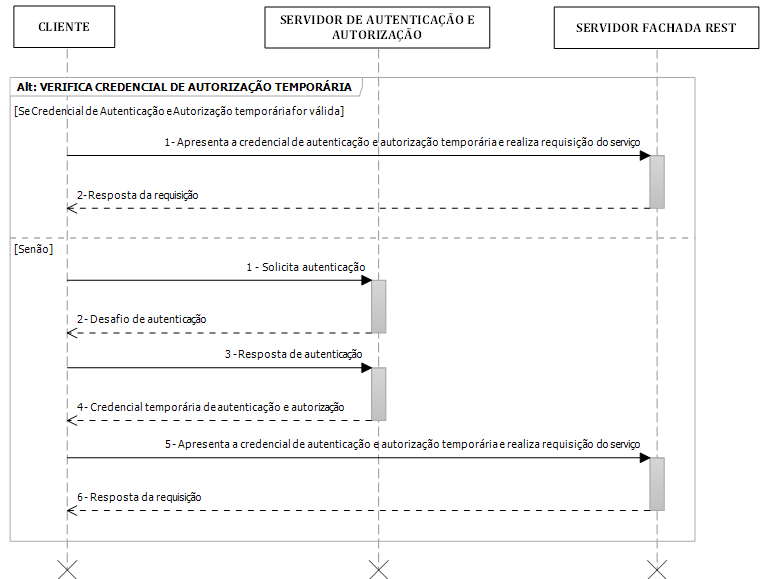
\includegraphics[width=0.8\textwidth]{cenario2_autenticacao.png}
%     \caption{Fluxo do protocolo de autenticação/autorização proposto, 2º cenário.}
%     \label{fig:cenario2}
%\end{figure}


\section{Formalização do protocolo}

O emprego de avaliações mais formais na área de criptografia não é recente. Grande parte dos trabalhos nesta área foram desenvolvidos na década de 90~\cite{Meadows95}. O emprego destes métodos possibilita uma análise completa do protocolo criptográfico e sua função principal é especificar se os objetivos propostos pelos autores são alcançados.

Neste trabalho, o protocolo proposto foi descrito formalmente, utilizando a lógica BAN, com o intuito de favorecer a comunicação e o entendimento utilizando uma linguagem mais precisa. Além disso, a propriedade de terminação com a geração da credencial temporária de autenticação e autorização foi verificada com um programa escrito em Prolog (ver Apêndice em anexo).


\section{Lógica BAN}

A lógica BAN foi desenvolvida por Burrows, Abadi e Needham em 1989, ela e uma das mais populares para a análise de crenças e de conhecimento entre os participantes dos protocolos criptográficos. É a primeira lógica a analisar formalmente os protocolos criptográficos,principalmente os de autenticação e distribuição de chaves~\cite{Burrows1990}.

\subsection{Notação básica}
Na lógica BAN, existem vários tipos distintos de objetos tais como entidades ou partes que se comunicam, chaves de criptografia e fórmulas lógicas. Uma fórmula lógica é uma versão idealizada da mensagem original, e às vezes ela pode ser referenciada como uma declaração lógica. Normalmente, os símbolos A, B e S denotam entidades ou participantes; $Kab$, $Kas$ e $Kbs$ denotam chaves compartilhadas; Ka, Kb e Ks denotam chaves públicas e $Ka^{-1}$, $Kb^{-1}$ e $Ks^{-1}$ denotam as chaves privadas dos participantes. Já $Na$, $Nb$ e $Ns$ são os identificadores gerados pelos participantes. As construções mais frequentemente utilizadas são apresentadas na Tabela~\ref{tab:notacaobasicaBAN}:

 \newcommand{\RHQuery}{\textbf{[???]}}
\newcommand{\RHRemark}[1]{\textbf{[#1]}}
\newcommand{\Believess}[2]{{#1}\mathrel{\textbf{\mid\equiv}}{#2}}
\newcommand{\Seess}[2]{{#1}\mathrel{\textbf{\triangleleft}}{#2}}
\newcommand{\Saids}[2]{{#1}\mathrel{\textbf{\mid\sim}}{#2}}

\newcommand{\Believes}[2]{{#1}\mathrel{\textbf{acredita}}{#2}}
\newcommand{\Sees}[2]{{#1}\mathrel{\textbf{recebeu}}{#2}}
\newcommand{\Said}[2]{{#1}\mathrel{\textbf{disse}}{#2}}
\newcommand{\Controls}[2]{{#1}\mathrel{\textbf{controla}}{#2}}
\newcommand{\Fresh}[1]{{#1}\,\textbf{novo}}
\newcommand{\Share}[3]{{#1}\stackrel{#2}{\longleftrightarrow}{#3}}
\newcommand{\ShareSecret}[3]{{#1}\stackrel{#2}{\rightleftharpoons}{#3}}
\newcommand{\PubKey}[2]{{}\stackrel{#1}{\mapsto}{#2}}
\newcommand{\Secret}[3]{{#1}\stackrel{#2}{\leftrightharpoons}{#3}}
\newcommand{\Encrypt}[2]{\{\,{#1}\,\}_{#2}}
\newcommand{\EncryptFrom}[3]{\{\,{#1}\,\}_{#2}^{#3}}
\newcommand{\Attach}[2]{\langle {#1}\rangle_{#2}}

%  \begin{tabular}{cp{16cm}}
\begin{table}[h]
    \begin{tabular}{|l|p{10cm}|}
    \hline
    \textbf{\emph{Expressão }}         & \textbf{\emph{Leitura/Significado}}                                                                               \\ \hline
    ${P}\mid\equiv{X}$               & $\Believes{P}{X}$: $P$ crê em $X$, ou $P$ acredita que $X$ é verdadeiro \\ \hline
    ${P}\triangleleft{X}$            & $\Sees{P}{X}$:Alguém enviou uma mensagem para $P$ contendo $X$ ou de outra forma $P$ recebeu $X$   \\ \hline
    ${P}\mid\sim{X}$                 & $\Said{P}{X}$:$P$ disse uma vez $X$. A entidade $P$ em algum momento enviou uma mensagem incluíndo a declaração $X$.\\ \hline
    ${P}\Rightarrow {X}$                 & $\Controls{P}{X}$:$P$ tem jurisdição sobre $X$. Onde $P$ é uma autoridade sobre $X$ é deve ser confiável \\ \hline
    \#(X)                            & novo$(X)$: a fórmula novo $X$, ela não foi usada numa mensagem anterior à execução protocolo atual.  \\ \hline
    $\Share{P}{k}{Q}$                & (lê-se ``k é uma chave satisfatória para $P$ e $Q$''). A chave $k$ nunca será descoberta por qualquer participante, exceto por P, Q ou por alguém em quem eles confiam \\ \hline
    $\{{X}\}_K$                  & fórmula $X$ foi cifrada com a chave $K$. As mensagens cifradas somente são legíveis e verificáveis pelo possuidor da chave \\ \hline
    $\ShareSecret{P}{k}{Q}$         & ${k}$ é o segredo compartilhado entre ${P}$ e ${Q}$ e possivelmente também com as entidades de confiança deles. Somente ${P}$ e ${Q}$ podem usar k para provar suas identidades \\ \hline
    $\PubKey{K}{P}$:               & ${k}$ é a chave pública de ${P}$  \\ \hline
    \end{tabular}
    \caption {Notação básica Lógica BAN, adaptação de ~\cite{Burrows1990}.}
\label{tab:notacaobasicaBAN}
\end{table}



\subsection{Postulados lógicos}

No estudo de protocolos de segurança é importante diferenciar o tempo das demonstrações ou eventos.  Haja vista que se isso não for observado, problemas, como a não detecção  do  reenvio de mensagens,  poderá acontecer.  Segundo~\cite{Burrows1990}, a lógica BAN trata dessa distinção dividindo-a em duas épocas: presente, que é o tempo durante a execução do protocolo, e o passado,  que refere-se às mensagens enviadas antes da execução do protocolo, o que faz com que elas sejam rejeitadas, uma vez que não são confiáveis .  Essa divisão de tempo é suficiente para facilitar o entendimento de como a lógica pode ser manipulada.
Para realizar a análise dos protocolos de segurança a lógica BAN possui uma serie de postulados lógicos, regras~\cite{Burrows1990}. Alguns deles  são descritos  a seguir:

\begin{enumerate}[ A )]

 \item Regra de significado da mensagem. Esta regra faz parte da interpretação das mensagens
    A1.1. Para as chaves secretas compartilhadas:
    \begin{displaymath}
        \infer
        {{P}\mid\equiv{{Q}\mid\sim{X}}}
        {{P}\mid\equiv{\Share{P}{k}{Q,}}& {P}\triangleleft{\Encrypt{X}{k}}}
        %{\Believes{P}{\Said{Q}{X}}}
        %{\Believes{P}{\Share{P}{k}{Q,}}&\Sees{P}{\Encrypt{X}{k}}}
    \end{displaymath}

    Se $P$ acredita que $k$ é uma chave satisfatória para se comunicar com $Q$ e se $P$ recebeu a mensagem $X$ cifrada com a chave $k$, então $P$ acredita que $Q$ uma vez disse $X$

    A1.2. De forma similar, aplicada a para as chaves públicas:

    \begin{displaymath}
        \infer
        {{P}\mid\equiv{{Q}\mid\sim{X}}}
        {{P}\mid\equiv{\PubKey{K}{Q}}& {P}\triangleleft{\Encrypt{X}{k ^{-1}}}}
                %{\Believes{P}{\Said{Q}{X}}}
                %{\Believes{P}{\Share{P}{k}{Q,}}&\Sees{P}{\Encrypt{X}{k}}}
    \end{displaymath}



\item Regra de verificação do identificador. Essa regra verifica se a mensagem é recente, se foi enviada durante a execução atual do protocolo e consequentemente, se o emissor acredita nela.

  \begin{displaymath}
    \infer
    {{P}\mid\equiv{{Q}\mid\equiv{X}}}
    {{P}\mid\equiv{\#(X),}& {P}\mid\equiv{{Q}\mid\sim{X}}}
    %{\Believes{P}{\Believes{Q}{X}}}
    %{\Believes{P} novo$(X),$ &\Believes{P}{\Said{Q}{X}}}
  \end{displaymath}

   Se $P$ acredita que $X$ é novo e $P$ acredita que em algum momento $Q$ disse $X$,então $P$ também acredita que $Q$ acredita em X.

\item Regra da jurisdição. Esta regra representa a confiança e a autoridade de uma entidade sobre as declarações.
\begin{displaymath}
    \infer
    {{P}\mid\equiv{X}}
    {{P}\mid\equiv{{Q}\Rightarrow {X},}& {P}\mid\equiv{{Q}\mid\equiv{X}}}
   % {\Believes{P}{X}}
   % {\Believes{P}{\Controls{Q}{X},} &\Believes{P}{\Believes{Q}{X}}}
  \end{displaymath}

   Se $P$  acredita que $Q$ tem jurisdição sobre a declaração $X$ e $P$ acredita que $Q$ acredita em $X$, então $P$ confia na declaração $X$.

\end{enumerate}

Estes são alguns dos principais postulados utilizados na construção da análise formal de protocolos criptográficos. A utilização destas regras juntamente com as notações descritas na sessão anterior possibilita que a crença dos participantes de um protocolo possa ser declarada.

\section{Análise formal do protocolo proposto}
Nesta sessão será realizado a análise formal do protocolo de autenticação e autorização proposto, utilizando a lógica BAN.

Na lógica BAN a análise de um protocolo é dividida em quatro etapas: A idealização do protocolo, que é originada a partir do protocolo original. As hipóteses, que são a suposições a respeito do estado inicial, nessa etapa são definidas as fórmulas lógicas que estão ligadas às declarações do protocolo, as declarações que são afirmações sobre o estado do sistema. As regras de inferência ou postulados lógicos que são aplicadas para os pressupostos e as afirmações a fim de descobrir as crenças detidas pelas partes no protocolo. %Normalmente, as premissas incluem as declarações sobre bens essenciais e partilha, geração de uso único e de confiança entre os diretores. nalanisisisisii %%http:www.tml.tkk.fi/Opinnot/Tik-110.501/1995/ban.html

\subsection{Idealização do protocolo}
\newcommand{\HT}[3]{\{\,{#1}\,\}\,{#2}\,\{\,{#3}\,\}}
\newcommand{\Msg}[3]{{#1}\longrightarrow{#2}:\,{#3}}

Para especificar o protocolo formalmente foram utilizadas algumas notações para representar os elementos participantes. Logo, os símbolos ${A}$, ${B}$ e ${C}$ são utilizadas para representar respectivamente as entidades, elementos participantes, que trocam mensagens: Cliente, Servidor REST e Servidor de Autenticação e Autorização. As chaves públicas das entidades ${A}$, ${B}$ e ${C}$ são representadas respectivamente por ${Ka}$, ${Kb}$ e  ${Kc}$. Já as chaves privadas, seguindo o mesmo pressuposto, são representadas pelos símbolos ${{Ka} ^{-1}}$, ${{Kb} ^{-1}}$ e ${{Kc} ^{-1}}$. Os elementos ${Cred_A}$ e ${Cod_{Srv_A}}$ representam respectivamente a credencial utilizada pela entidade ${A}$ e o código que identifica o serviço que a entidade ${A}$ está requerendo.

O desafio gerado pela entidade ${C}$ é enviado a entidade ${A}$ e representado pela fórmula ${N_{CA}}$ que corresponde aos elementos: Código do Desafio gerado pela entidade ${C}$ e Código da Credencial aleatória da entidade ${A}$. A resposta do desafio gerada pela entidade ${C}$ à entidade ${A}$ é representado  pelo símbolo ${Resp_{AC}}$ que corresponde aos elementos: Código do Desafio gerado pela entidade ${C}$ e Credencial Solicitada da entidade ${A}$. ${Ts_A}$ e ${Ts_C}$ são respectivamente os \emph{timestamps} emitidos pelas entidades ${A}$ e ${C}$.

O símbolo ${Msg_{AC}}$ representa o resumo da mensagem enviada pela entidade ${A}$ a entidade ${C}$,  ${Msg_{CA}}$ representa o resumo da mensagem enviada pela entidade ${C}$ a entidade ${A}$ e ${Msg_{AB}}$ representa o resumo da mensagem enviada pela entidade ${A}$ a entidade ${B}$. O elemento ${H}$ representa o \emph{hashing} aplicado a uma mensagem utilizando o algoritmo SHA3.

E finalmente, o símbolo ${Exp_A}$ representa a data/hora  de expiração da Credencial Temporária de autorização e autenticação, ${C_{Aut}}$ corresponde à credencial temporária de autorização e autenticação gerada para a entidade A e ${Req_A}$, que refere-se à requisição de serviço de A ( Get, Put, Post ou Delete).

Para especificar formalmente um protocolo de segurança utilizando a lógica BAN, é necessário primeiro idealizar o protocolo, objeto da análise, e a partir da aplicação dos postulados e das suposições iniciais verificar se ele atinge ou não o seu objetivo. A idealização do protocolo proposto e descrito na figura ~\ref{fig:protocoidealizado} e representa o fluxo de troca de mensagens executado pelo protocolo. Todas as mensagens são consideradas na análise, pois utilizam criptografia assimétrica desde a primeira troca de mensagens.

\begin{figure}[!htb]
    \centering
    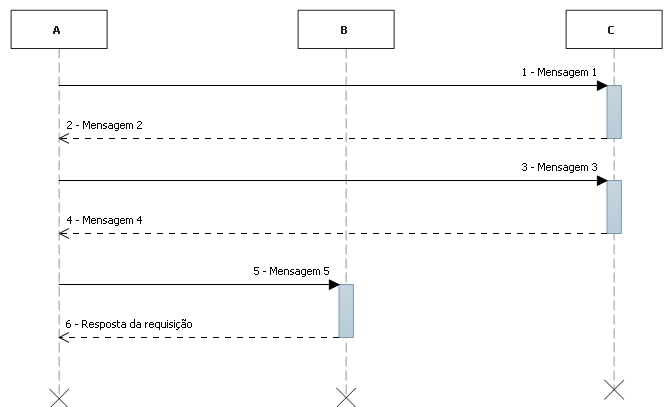
\includegraphics[width=0.8\textwidth]{fluxo_autenticacao_BAN.png}
    \caption{Diagrama de idealização do protocolo de autenticação/autorização proposto}
    \label{fig:protocoidealizado}
\end{figure}

\begin{enumerate}
  \item Mensagem 1: $\Msg{A}{C}{\Encrypt{Ts_A,Cred_A,H{\Encrypt{Msg_{AC}}{Ka ^{-1}}}}{Kc}}$.
  \item Mensagem 2: $\Msg{C}{A}{\Encrypt{Ts_C,{N_{CA}},H{\Encrypt{Msg_{CA}}{Kc ^{-1}}}}{Ka}}$.
  \item Mensagem 3: $\Msg{A}{C}{\Encrypt{Ts_A,{Resp_{AC}},Cod_{Srv_A},H{\Encrypt{Msg_{AC}}{Ka ^{-1}}}}{Kc}}$.
  \item Mensagem 4: $\Msg{C}{A}{\Encrypt{Ts_C,Exp_A,\#(\ShareSecret{A}{{C_{Aut}}}{C}),H{\Encrypt{Msg_{CA}}{Kc ^{-1}}}}{Ka}}$.
  \item Mensagem 5: $\Msg{A}{B}{\Encrypt{Ts_A,(\ShareSecret{A}{{C_{Aut}}}{C}),H{\Encrypt{Msg_{AB}}{Ka ^{-1}}}}{Ka}},{Req_A}$.
\end{enumerate}
\subsection{Suposições}\label{sec:Suposicoes}
O objetivo do protocolo é fazer que a entidade ${A}$ seja autenticada pela entidade ${C}$ e obtenha uma credencial de autenticação e autorização temporária referente a uma requisição de um serviço que a entidade ${A}$ deseja consumir. De forma que a credencial de autenticação e autorização temporária  possa ser utilizada pela entidade ${A}$ no momento da requisição do serviço a entidade ${B}$ e obtenha o que deseja. Para isso, algumas suposições iniciais são estabelecidas e juntamente com a aplicação  dos postulados da lógica BAN, busca-se concluir que o protocolo alcance o objetivo proposto. Todas as suposições, apresentadas na Tabela~\ref{tab:suposicoesBAN} são baseadas em um canal seguro de comunicação SSL/TSL, onde tanto o receptor  quanto o emissor do serviço são conhecidos e autenticados usando-se certificados digitais X.509.

\begin{table}[h]
\begin{tabular}{cllcl}
\textbf{Suposição} & \textbf{Descrição} &  & \textbf{Suposição} & \textbf{Descrição} \\
\textbf{1 -}       & $ A \mid\equiv$  ${\PubKey{Kc}{C}}$                 &  & \textbf{9 -}       & $ B \mid\equiv$ $ C \Rightarrow $ $\#(\ShareSecret{A}{{C_{Aut}}}{C})$ \\
\textbf{2 -}       & $ B \mid\equiv$  ${\PubKey{Ka}{A}}$                 &  & \textbf{10 -}      & $ A \mid\equiv$ $ C \mid\equiv $ $\#(\ShareSecret{A}{{C_{Aut}}}{C})$ \\
\textbf{3 -}       & $ C \mid\equiv$  ${\PubKey{Ka}{A}}$                 &  & \textbf{11 -}      & $ B \mid\equiv$ $ C \mid\equiv $ $\#(\ShareSecret{A}{{C_{Aut}}}{C})$ \\

\textbf{4 -}       & $ A \mid\equiv$  $\#{Ts_C}$                         &  & \textbf{12 -}      & $ A \mid\equiv$  $\#(\ShareSecret{A}{{C_{Aut}}}{C})$  \\

\textbf{5 -}       & $ B \mid\equiv$  $\#{Ts_A}$                         &  & \textbf{13 - }      & $ B \mid\equiv$  $\#(\ShareSecret{A}{{C_{Aut}}}{C})$  \\

\textbf{6 -}       & $ C \mid\equiv$  $\#{Ts_A}$                         &  & \textbf{ }                    &                                      \\
\textbf{7 -}       & $ A \mid\equiv$  ${Exp_A}$                          &  & \textbf{ }                   &
\\
\textbf{8 -}       & $ A \mid\equiv$  $ C \Rightarrow $ $\#(\ShareSecret{A}{{C_{Aut}}}{C})$   &   & \textbf{ }     &                               \\
\end{tabular}
\caption {Suposições aplicadas ao protocolo proposto.}
\label{tab:suposicoesBAN}
\end{table}


Dessa forma, temos que as suposições 1,2 e 3 garantem que as entidades participantes ${A}$, ${B}$ e ${C}$ confiam  nas chaves públicas das entidades que farão as trocas de mensagem. As suposições 4, 5 e 6 são \emph{timestamps}, o que denota que as entidades ${A}$, ${B}$ e ${C}$ devem estar sincronizadas. Sendo assim, a entidade ${A}$ acredita que o \emph{timestamp} ${Ts_C}$ é novo e foi gerado recentemente. Da mesma forma que as entidades ${B}$ e ${C}$ acreditam  que o \emph{timestamp} ${Ts_A}$ também é novo e foi gerado recentemente. A suposição 7 é utilizada pela entidade ${A}$ para garantir que a credencial de autenticação e autorização gerado pela entidade ${C}$ não expirou e que pode ser utilizada. As suposições 8 e 9 denotam que as entidades ${A}$, ${B}$ acreditam que entidade ${C}$ tem jurisdição  sobre a credencial de autenticação e autorização gerada. Portanto, as suposições 10 e 11 garantem que as entidades ${A}$, ${B}$ acreditam que a credencial de autenticação e autorização gerada é nova é foi realmente gerada pela entidade ${C}$. Finalmente, as suposições 12 e 13 garantem que as entidades ${A}$, ${B}$ acreditam na nova credencial de autenticação e autorização temporária, ${C_{Aut}}$.

\subsection{Provas}

Como o objetivo final do protocolo é autenticar a entidade ${A}$, de forma que ela obtenha uma credencial de autenticação e autorização temporária, referente a uma requisição de serviço desejado. Será realizado uma análise de cada mensagem  do protocolo idealizado. Para isso, serão aplicados os postulados lógicos e suposições, a fim de provar que o protocolo consegue atingir o objetivo proposto.

Na primeira mensagem, a entidade ${A}$ envia sua credencial, um \emph{timestamp} e o código do serviço que ele está querendo consumir ao servidor de autenticação e autorização, representado pela entidade ${C}$. A mensagem enviada é assinada com a chave privada do participante ${A}$  e cifrada com a chave pública do participante ${C}$. Esse processo e descrito a seguir:

\textbf{Mensagem 1}: $\Msg{A}{C}{\Encrypt{Ts_A,Cred_A,H{\Encrypt{Msg_{AC}}{Ka ^{-1}}}}{Kc}}$.

$C\triangleleft$ ${\Encrypt{Ts_A,Cred_A,Cod_{Srv_A},H{\Encrypt{Msg_{AC}}{Ka ^{-1}}}}{Kc}}$

$C\mid\equiv A \mid\sim $  $H\{Msg_{AC}\}$

$C\mid\equiv A \mid\sim$ ${\#Ts_A}$

$C\mid\equiv$ ${Cred_A,Cod_{Srv_A}}$

Sendo assim, ${\textbf{C}}$ recebe a fórmula ${\Encrypt{Ts_A,Cred_A,Cod_{Srv_A},H{\Encrypt{Msg_{AC}}{Ka ^{-1}}}}{Kc}}$, e usando sua chave privada, decifra a fórmula recebida. Após decifrar a fórmula, e aplicando a regra do significado da mensagem na suposição 3 usando a função $H \{Msg_{AC}\}$ confirma a autenticidade e integridade da mensagem. Por fim, aplica a regra de verificação do identificador na suposição 6 usando a fórmula ${Ts_A}$ para obter a credencial da entidade ${A}$ :  ${Cred_A}$.

Resultado:

${C}$ obtém  a credencial da entidade $A$: ${Cred_A}$

Na segunda mensagem, após receber e validar os dados enviados por $A$, a entidade ${C}$ gera um desafio de autenticação, ${N_{CA}}$. O desafio consiste em fazer uma busca aleatória à tabela de credenciais e selecionar um código de credencial que esteja associado a entidade $A$. Em seguida grava-se o desafio, a data e hora de geração do desafio e a resposta esperada em uma base de dados. Na sequência, uma mensagem, contendo o desafio e um \emph{timestamp}, é enviada a entidade $A$, assinada com a chave privada da entidade ${C}$ e cifrada com a chave pública da entidade ${A}$. Logo temos:

\textbf{Mensagem 2}: $\Msg{C}{A}{\Encrypt{Ts_C,{N_{CA}},H{\Encrypt{Msg_{CA}}{Kc ^{-1}}}}{Ka}}$.

$\textbf{A}\triangleleft$ ${\Encrypt{Ts_C,{N_{CA}},H{\Encrypt{Msg_{CA}}{Kc ^{-1}}}}{Ka}}$

$\textbf{A}\mid\equiv \textbf{C} \mid\sim $  $H \{Msg_{CA}\}$

$\textbf{A}\mid\equiv \textbf{C} \mid\sim$ ${Ts_C}$

$\textbf{A}\mid\equiv$ ${N_{CA}}$

A entidade ${\textbf{A}}$ recebe a fórmula ${\Encrypt{Ts_C,{N_{CA}},H{\Encrypt{Msg_{CA}}{Kc ^{-1}}}}{Ka}}$ e a decifra usando sua chave privada, em seguida aplicando a regra do significado da mensagem na suposição 1 usando a função $H \{Msg_{CA}\}$ confirma a autenticidade e integridade da mensagem. Por fim, aplica a regra de verificação do identificador na suposição 4 e usando a fórmula ${Ts_C}$ para obter o desafio,${N_{CA}}$, gerado pela entidade ${C}$.

Resultado:

${A}$ obtém  o desafio de autenticação gerado pela entidade ${C}$: ${N_{CA}}$

Na terceira mensagem, a entidade ${A}$, após receber e validar o desafio gerado pela entidade ${C}$, envia a resposta ${Resp_{AC}}$, conforme solicitado. Essa resposta consiste em informar o código do desafio gerado pela entidade ${C}$ e a credencial associada ao código de credencial solicitada pela entidade ${C}$. Além disso, a entidade ${A}$ deve informar o código do serviço que deseja consumir. Sendo assim, temos:

\textbf{Mensagem 3}: $\Msg{A}{C}{\Encrypt{Ts_A,{Resp_{AC}},Cod_{Srv_A},H{\Encrypt{Msg_{AC}}{Ka ^{-1}}}}{Kc}}$.

$C\triangleleft$ ${\Encrypt{Ts_A,{Resp_{AC}},H{\Encrypt{Msg_{AC}}{Ka ^{-1}}}}{Kc}}$

$C\mid\equiv A \mid\sim $  $H \{Msg_{AC}\}$

$C\mid\equiv A \mid\sim$ ${\#Ts_A}$

$C\mid\equiv$ ${Resp_{AC}}$

${\textbf{C}}$ recebe a fórmula ${\Encrypt{Ts_A,{Resp_{AC}},H{\Encrypt{Msg_{AC}}{Ka ^{-1}}}}{Kc}}$, e a decifra usando sua chave privada, em seguida aplicando a regra do significado da mensagem na suposição 3 usando a função $H \{Msg_{AC}\}$ confirma a autenticidade e integridade da mensagem. Por fim, aplica a regra de verificação do identificador na suposição 6 usando a fórmula ${Ts_A}$ para obter os dados da resposta do desafio ${Resp_{AC}}$, e assim, validar a resposta enviada e autenticar a entidade ${A}$. Dando início ao processo de autorização.

Resultado:

${C}$ autentica a entidade ${A}$.

Na mensagem 4, após autenticar a entidade ${A}$, a entidade ${C}$ procede com o processo de autorização, que consiste em verificar qual serviço a entidade está querendo consumir, para isso verifica o código de serviço solicitado pela entidade ${A}$, $Cod_{Srv_A}$, que foi informado no envio da mensagem 3. Se a entidade ${A}$ possuir privilégios necessários para consumir o serviço requisitado, a entidade ${C}$ gera uma nova credencial de autorização temporária para o serviço solicitado. Em seguida, a entidade ${C}$ grava a credencial ${(\ShareSecret{A}{{C_{Aut}}}{C})}$, o código do serviço que a entidade ${A}$ está requerendo, a data e hora de criação, a data de expiração e o código do contrato da entidade ${A}$. Terminado esse procedimento, a entidade ${C}$, envia, uma mensagem contendo a credencial ${(\ShareSecret{A}{{C_{Aut}}}{C})}$, a data e hora de expiração da credencial,${Exp_A}$ e um \emph{timestamp} a entidade ${A}$. Esta mensagem é assinada com a privada da entidade ${C}$ e cifrada com a chave pública da entidade ${A}$. Logo temos:

\textbf{Mensagem 4}: $\Msg{C}{A}{\Encrypt{Ts_C,Exp_A,\#(\ShareSecret{A}{{C_{Aut}}}{C}),H{\Encrypt{Msg_{CA}}{Kc ^{-1}}}}{Ka}}$.

$\textbf{A}\triangleleft$ $\Msg{C}{A}{\Encrypt{Ts_C,Exp_A,\#(\ShareSecret{A}{{C_{Aut}}}{C}),H{\Encrypt{Msg_{CA}}{Kc ^{-1}}}}{Ka}}$.

$\textbf{A}\mid\equiv \textbf{C} \mid\sim $  $H \{Msg_{CA}\}$

$\textbf{A}\mid\equiv \textbf{C} \mid\sim$ ${Ts_C}$

$\textbf{A}\mid\equiv \textbf{C} \mid\sim$ ${Exp_A}$

$\textbf{A}\mid\equiv \textbf{C} \Rightarrow $  ${\#(\ShareSecret{A}{{C_{Aut}}}{C})}$

$\textbf{A}\mid\equiv \textbf{C} \mid\equiv $  ${\#(\ShareSecret{A}{{C_{Aut}}}{C})}$

$\textbf{A}\mid\equiv$ ${\#(\ShareSecret{A}{{C_{Aut}}}{C})}$

A entidade ${A}$ recebe a fórmula ${\Encrypt{Ts_C,Exp_A,\#(\ShareSecret{A}{{C_{Aut}}}{C}),H{\Encrypt{Msg_{CA}}{Kc ^{-1}}}}{Ka}}$, e a decifra usando sua chave privada, em seguida aplicando a regra do significado da mensagem na suposição 1 usando a função $H \{Msg_{CA}\}$ confirma a autenticidade e integridade da mensagem. Ela aplica a regra de verificação do identificador nas suposições 4 e 7 usando as fórmulas ${Ts_C}$  e ${Exp_A}$. E, finalmente, aplicando a regra da jurisdição, nas suposições 7 e 9, obtém a credencial de autorização temporária ${\#(\ShareSecret{A}{{C_{Aut}}}{C})}$.

Resultado:

${\textbf{A}}$ obtém a credencial de autorização temporária: ${\#(\ShareSecret{A}{{C_{Aut}}}{C})}$.

Finalmente, na quinta mensagem, a entidade ${A}$ após receber e validar a mensagem enviada pela entidade ${C}$, obtendo assim a credencial de autenticação e autorização temporária, ${\#(\ShareSecret{A}{{C_{Aut}}}{C})}$, envia uma mensagem a entidade ${B}$  contendo a requisição do serviço que deseja consumir juntamente com a credencial de autorização temporária. Esta mensagem é assinada com a chave privada da entidade ${A}$ e cifrada com a chave pública da entidade ${B}$. Logo temos:

\textbf{Mensagem 5}: $\Msg{A}{B}{\Encrypt{Ts_A,(\ShareSecret{A}{{C_{Aut}}}{C}),H{\Encrypt{Msg_{AB}}{Ka ^{-1}}}}{Kb}},{Req_A}$.

$\textbf{B}\triangleleft$  ${\Encrypt{Ts_A,(\ShareSecret{A}{{C_{Aut}}}{C}),H{\Encrypt{Msg_{AB}}{Ka ^{-1}}}}{Kb}},{Req_A}$

$\textbf{B}\mid\equiv \textbf{A} \mid\sim $  $H\{Msg_{AB}\}$

$\textbf{B}\mid\equiv \textbf{A} \mid\sim$ ${Ts_A}$

$\textbf{B}\mid\equiv \textbf{A} \Rightarrow $  ${\#(\ShareSecret{A}{{C_{Aut}}}{C})}$

$\textbf{B}\mid\equiv \textbf{A} \mid\equiv $  ${\#(\ShareSecret{A}{{C_{Aut}}}{C})}$

$\textbf{B}\mid\equiv$ ${\#(\ShareSecret{A}{{C_{Aut}}}{C})}$

A entidade ${\textbf{B}}$ recebe a fórmula ${\Encrypt{Ts_A,(\ShareSecret{A}{{C_{Aut}}}{C}),H{\Encrypt{Msg_{AB}}{Ka ^{-1}}}}{Kb}},{Req_A}$, e a decifra, usando sua chave privada. Em seguida aplicando a regra do significado da mensagem na suposição 2 usando a função $H\{Msg_{AB}\}$ confirma a autenticidade e integridade da mensagem. Ela aplica a regra de verificação do identificador na suposições 5 usando as fórmulas ${Ts_A}$. E, finalmente, aplicando a regra da jurisdição, nas suposições 8 e 10, obtém a credencial de autorização temporária ${\#(\ShareSecret{A}{{C_{Aut}}}{C})}$ e autoriza a entidade \textbf{A} a consumir a requisição ${Req_A}$.

Conclusão :

${B}$ autoriza ${A}$ a partir da nova credencial ${(\ShareSecret{A}{{C_{Aut}}}{C})}$ a consumir a requisição ${Req_A}$

\subsection{Análise}

A análise demonstra que o protocolo de autenticação e autorização proposto alcança os objetivos propostos na Seção~\ref{sec:Suposicoes}, que é a autenticação da entidade ${A}$ e a emissão da credencial de autenticação e autorização temporária. Isso permite que a entidade ${A}$ consuma o serviço requerido. É importante frisar que a lógica BAN foi utilizada para demonstrar a execução do protocolo e que a utilização da lógica é apenas um dos passos necessários para verificar se existem possíveis falhas no protocolo.

Para verificar a segurança do protocolo é necessário que seja empregado um método de criptoanálise sobre a criptografia utilizada e assim verificar quais são vulnerabilidades que o protocolo ou os algoritmos criptográficos empregados estão sujeitos.


\section{Implementação}\label{sec:implementacao}

Após a definição do protocolo proposto e para atender a necessidade da realização de testes de desempenho que tem a finalidade de avalizar o impacto da solução proposta no oferecimento de serviços pela PCDF, surgiu a necessidade da criação de um protótipo do protocolo de autenticação e autorização proposto. Esse protótipo foi desenvolvido em conjunto com o corpo acadêmico da UNB, neste caso, o responsável pelo desenvolvimento foi o aluno Alexandre Lucchesi.  A descrição desse protótipo e apresentado a seguir.
\subsection{Protótipo}

Para implementar o protótipo do protocolo proposto foi necessário desenvolver cada um dos componentes: Cliente, Servidor de Autenticação e Autorização e Servidor REST, descritos na arquitetura do protocolo na seção~\ref{sec:ArqProtocolo}. Para isso, foi utilizada a linguagem de programação puramente funcional Haskell, com o compilador GHC(Glasgow Haskell Compiler) versão 7.6.3. Para o controle de dependências e gerenciamento de \emph{build} de aplicações foi utilizado à ferramenta Cabal que é um o gerenciador de pacotes do Haskell. Com ele é possível construir aplicações e bibliotecas de forma padronizada, organizada e portável. Para criar o protótipo ainda foi utilizado o framework Haskell para desenvolvimento web, denominado Snap \emph{Framework} que é necessário para manipulação de requisições e respostas HTTP, que são utilizadas pelo protocolo de autenticação e autorização proposto. Além disso, foi utilizado o HsOpenSSL que é um OpenSSL vinculativo para Haskell, utilizado para garantir a utilização do HTTPS em todas as trocas de mensagem a partir de código Haskell.

Para a assinatura digital das mensagens utilizadas pelo protocolo foi utilizado o algoritmo RSASSA\-PKCS\-v1\_5 SHA\-256 conforme orientação descrita na publicação~\cite{ietfjws} e para criptografia foi utilizado o algoritmo de criptografia assimétrica, RSAES\-PKCS1\-V1\_5, para cifrar a chave simétrica utilizada no algoritmo de criptografia simétrica AES\_128\_CBC\_HMAC\_SHA\_256 que foi utilizado para cifrar a mensagem. Procurou-se seguir a orientação do que é preconizado na publicação~\cite{jwt2014}.

O servidor de banco de dados foi implementado utilizando o banco de dados não relacional \emph{Apache CouchDB}, que é um banco de dados flexível e tolerante a falhas que usa \emph{JSON} para armazenar os dados, JavaScript como sua linguagem de consulta usando o MapReduce, além disso, este banco de dados oferece API estilo REST.

O protótipo implementado não objetivou a otimização do protocolo, seu objetivo foi o de possibilitar a realização dos testes de desempenho e de verificar as funcionalidades do protocolo proposto.

\section{Análise de Segurança}

Nesta seção serão discutidas as propriedades de segurança do protocolo de autenticação e autorização proposto. São abordadas as propriedades e alguns ataques que podem ser realizados contra ele. Essa seção segue o padrão determinado no trabalho~\cite{traust08}.

\subsection{Segurança da sessão}

O protocolo de Autenticação e Autorização proposto utiliza para segurança de seção e da camada de transporte, o protocolo TLS/SSL. A utilização desse protocolo tem por objetivo evitar o ataque man-in-the-middle. Para isso, é exigido tanto do órgão conveniado como da própria PCDF que ambas utilizem certificados digitais padrão X.509 emitidos e garantidos por uma AC que esteja subordinada à hierarquia da ICP-Brasil.

Com isso, ambas as partes envolvidas no processo de comunicação podem estabelecer um processo de confiança mútua no nível de transporte. Todo o tráfego que flui sobre uma sessão bilateral certificada tem uma fonte confiável. Isso permite que implementações de serviços possam autorizar ou desautorizar interações com base na fonte bem conhecida de uma solicitação HTTP.

Além da segurança oferecida pela utilização da segurança na camada de transporte, com utilização do TLS/SSL, o protocolo utiliza mecanismos de segurança tais como criptografia assimétrica e assinatura digital. Isso Permite que outras partes mal intencionadas não consigam ter acesso ao conteúdo das mensagens trocadas pelo protocolo no processo de comunicação.

Diferentemente do sistema Traust, o protocolo de Autenticação e Autorização proposto, não será executado em ambientes em que nem o cliente nem o servidor tem uma chave pública certificada, procura-se dessa forma, atenuar problemas relacionados ao protocolo TLS, que quando executado em ambientes em que nem o cliente nem o servidor tem uma chave pública certificada, pode ser vulnerável a um ataque man-in-the-middle durante o estabelecimento da sessão~\cite{traust08}.

\subsection{Responsabilização dos usuários conveniados}

Uma das ameaças verificadas diz respeito a possibilidade do uso indevido, por parte dos órgãos conveniados, das informações disponibilizadas nos serviços ofertados pela PCDF. Isso decorre do fato das informações disponibilizadas serem sensíveis e possuírem caráter sigiloso. Dessa forma, para evitar esse problema é exigido dos órgãos conveniados que assinem um contrato para o consumo do serviço. No momento da assinatura do contrato eles recebem uma tabela contendo várias credenciais que servem como identidades e que deverão ser utilizadas no processo de autenticação, conforme descrito no seção~\ref{sec:reqprotocolo}. Isso possibilita que haja uma autenticação mútua entre a PCDF e os consumidores dos serviços. Além disso, com a utilização do protocolo de autenticação e autorização proposto, são empregados mecanismos de criptografia e assinaturas digitais que são geradas a partir de certificados digitais padrão X.509 vinculados aos órgãos e garantidos por AC. Dessa forma, busca-se evitar o não-repúdio por parte dos órgãos conveniados, atribuindo-lhes responsabilidades em caso do mau uso dos serviço ofertados pela PCDF.

Logo, uma vez detectado algum tipo de vazamento de dados proveniente dos serviços ofertados o órgão poderá ser identificado e após uma apuração minuciosa, responsabilizado pelos danos causados à PCDF.

\subsection{Ataques de repetição}
Esta ameaça, conforme descrito no capitulo~\ref{cap:revisaolit}, seção~\ref{sec:vulnerabilidadessoa}, se empregada contra o protocolo de autenticação e autorização proposto, tem uma chance quase nula de sucesso. Uma vez que são empregados \emph{timestamps} em em todas as trocas de mensagens realizadas pelo protocolo. Além disso, são gerados números únicos, que identificam os desafios de autenticação gerados e podem ser utilizados como \emph{nonces}, que também podem ser empregados contra esse tipo de ataque.

\subsection{Ataques de negação de serviço}

Esta ameaça é muito difícil de ser evitada, haja vista que,  pode ser fruto de ataques via rede, do consumo excessivo de recursos da máquina,  ou ainda,  ser resultante da exploração de qualquer tipo de vulnerabilidade que implique na indisponibilidade do serviço ou de um recurso. O protocolo de autenticação e autorização proposto é baseado no esquema de desafio-resposta. Os desafios são gerados de forma aleatória a partir das credenciais que identificam unicamente os consumidores dos serviços, o que possibilita uma autenticação mútua. Além disso, também são empregados outros mecanismos de segurança como utilização da segurança na camada de transporte e mecanismos de criptografia e assinaturas digitais. Isso minimiza a ameaça de ataques de negação de serviço.

Assim como o sistema Traust,~\cite{traust08}, o servidor de autenticação e autorização proposto pode ser replicado para outros servidores, o que possibilita um balanceamento de carga e minimiza a criação de gargalos. Isso permite que o servidor de autenticação seja escalável e esteja disponível em situações críticas, como no caso dos ataques de negação de serviço.


\subsection{Roubo de credenciais de autenticação e autorização}\label{subsec:RouboCred}

O protocolo de autenticação a autorização proposto após executado corretamente emite um token de segurança que será utilizado para a obtenção do serviço desejado, conforme apresenato na seção~\ref{sec:ArqProtocolo}, cabe ressaltar que se por algum motivo um atacante, conseguir burlar o os mecanismos de segurança utilizados pelo protocolo e conseguir acesso a essa credencial de autenticação e autorização ele terá acesso apenas um serviço, pois o protocolo emite credenciais para um único serviço por vez e com tempo de expiração determinado no momento de sua geração.

Essa é uma situação muito difícil de ser verificada, porém caso ocorra o problema é minimizado e não terá grande impacto na arquitetura do protocolo como um todo.

Outro problema que pode ocorrer é o roubo de credenciais de autenticação, que são as credenciais que o órgão conveniado recebe no momento da assinatura do contrato de oferecimento do serviço. Essa credenciais são utilizadas para responder os desafios que serão realizadas pelo protocolo de autenticação proposto. Caso isso ocorra e seja identificado a PCDF pode de forma rápida e transparente desativar as credenciais que julgar que foram comprometidas sem que o usuário seja prejudicado. Em um caso mais extremo, outras podem ser geradas e redistribuíras ao órgão conveniado.

Porém cabe ressaltar que caso ocorra o roubo de credenciais, o órgão que teve o problema será investigado e poderá ser responsabilizado se for detectado má fé má gestão na guarda das credenciais, conforme descrito na subseção~\ref{subsec:RouboCred}


\subsection{Ponto único de ataque}

Uma das possibilidades verificadas é que ocorrendo um ataque, o alvo possa não ser protocolo de autenticação e autorização proposto e sim o próprio servidor de autenticação e autorização. Neste caso, se o atacante for bem sucedido em sua empreitada o servidor poder ficar vulnerável. Esse servidor é responsável pela geração dos desafios de autenticação e pela geração das credenciais de autenticação e autorização. Porém, apesar de realizar estas atividades ele armazena e consulta os dados gerados no processo de autenticação e autorização em outra máquina, que é em um servidor de banco de dados. Em outras palavras o servidor de autenticação e autorização está em uma máquina diferente do servidor de banco de dados, o que minimiza os problemas relacionados a esse tipo de ataque, pois o servidor pode ser replicado para outra máquina e o que estiver com problemas pode ser fácilmente substituído.
\section{Síntese do capítulo}

Este capítulo apresentou os requisitos e a arquitetura do protocolo de autenticação e autorização proposto.  Além disso,  o capítulo apresentou a formalização do protocolo utilizando à lógica BAN.  Foi descrita de forma sucinta a implementação de um protótipo do protocolo proposto. Ao final foi realizada uma análise de segurança semelhante ao do trabalho proposto em~\cite{traust08}. No próximo capítulo será realizada uma análise de desempenho a fim de mensurar o impacto do protocolo na infraestrutura da PCDF. 
  \chapter{Protocolo de Autenticação e Autorização Proposto}\label{cap:Protocolo}

%A Polícia Civil do Distrito Federal, diante da necessidade de compartilhar suas informações com órgão parceiros, no intuito de possibilitar que os sistemas possam ser integrados de forma eficiente e principalmente segura busca estabelecer uma arquitetura de referência para a adoção de uma arquitetura orientada a serviços. Essa arquitetura deve primar pela segurança, haja vista a criticidade e sensibilidade das informações que são tratadas no âmbito da PCDF.

%Dessa forma, optou-se por adotar a tecnologia de Web Services usando o protocolo REST para implementar SOA na instituição. Neste caso, estudos específicos foram realizados com vistas a estabelecer uma política de segurança eficiente que possibilite o fornecimento dos serviços e promova a integração com os órgãos parceiros.

A Polícia Civil do Distrito Federal, diante da necessidade de compartilhar suas informações com órgãos parceiros, de forma eficiente e segura, objetiva estabelecer uma arquitetura de referência para a adoção de uma arquitetura orientada a serviços. Essa arquitetura deve primar pela segurança, dada a criticidade e sensibilidade das informações que são tratadas no âmbito da PCDF, conforme discutido no capítulo~\ref{sec:introducao}.
Dessa forma, para implementar uma arquitetura orientada a serviços na Instituição optou-se pela adoção de uma solução baseada no modelo REST, que é escalável e possibilita a otimização de desempenho dos serviços, uma vez que pode utilizar formatos de mensagem mais leves, como por exemplo, o \emph{JavaSript Objetc Notation}(JSON), conforme apresentado no capítulo~\ref{cap:revisaolit} e seção~\ref{sec:rest}. Neste cenário, essa dissertação contribui com um protocolo de autenticação e autorização que atende às necessidades particulares da PCDF, mas que também pode ser adotado em outras instituições. Este capítulo inicia com a apresentação dos requisitos do protocolo e de sua arquitetura, onde é apresentada uma visão geral do Protocolo de Autenticação e Autorização proposto. Em seguida é realizada a análise formal do protocolo utilizando-se a lógica BAN. Por fim, este capítulo termina com a descrição da implementação de um protótipo do protocolo proposto.


\section{Requisitos do Protocolo}\label{sec:reqprotocolo}

O protocolo de autenticação e autorização deve ser aderente à arquitetura REST, haja vista que sua adoção é fácil, pois pode ser implementada em várias linguagens e em diferentes sistemas operacionais.  Além disso, permite utilizar o formato de mensagem JSON, que é o formato de mensagem padrão utilizado pelo Protocolo de Autenticação e Autorização proposto. Os requisitos inerentes ao protocolo são descritos nesta seção.

\begin{enumerate}[RQ1]

\item Segurança de sessão. Toda comunicação entre o cliente e o servidor deve ser realizada utilizando HTTPS
\emph{(Hypertext Transfer Protocol over Secure Sockets Layer)}, usando o SSL/TLS para garantir a confidencialidade
e integridade para a sessão. Para isso será usado o certificado digital X.509 tipo A3, emitido por uma Autoridade Certificadora(CA), que esteja subordinada à hierarquia da ICP-Brasil, para encriptar as comunicações e garantir a autenticidade do servidor e do cliente. Os clientes devem realizar a validação do certificado antes de interagir com o servidor.

\item Segurança na troca de mensagens. Deve ser utilizada criptografia assimétrica, para promover a segurança na troca de mensagens realizada entre o Cliente e a PCDF. Todas as mensagens deverão ser assinadas digitalmente. Para isso, será utilizado uma função \emph{Hash}, com o algoritmo SHA (Secure Hash Algorithm).

\item Autorização e escalabilidade. O protocolo deve permitir acesso aos serviços ofertados apenas às instituições autorizadas. Desta forma, a autenticação e autorização devem seguir os padrões definidos na política de segurança estabelecida pela PCDF. Logo, para ser autenticado, o usuário deve apresentar credenciais válidas, que são declarações de identidade (\emph{Claims}), que serão utilizadas no processo de autenticação e autorização. Essas credenciais devem ser criptografadas, assinadas e enviadas no cabeçalho do protocolo HTTPS.
    O protocolo de autenticação e autorização proposto deve ser escalável em termos de sobrecarga, tamanho do domínio de proteção e de manutenção. Além disso, o protocolo deve permitir a preservação de privacidade, uma vez que para proteger as instituições e a PCDF de entidades maliciosas, suas interações deverão revelar o mínimo de informações possíveis.

\item Flexibilidade. A autenticação e autorização deve ser baseada em desafios e resposta, que serão elaborados a partir da apresentação de declarações de identidades (\emph{Claims}). Este requisito torna mais flexível o gerenciamento da identidade do usuário, uma vez que possibilita ao administrador desabilitar credenciais que tenham sido comprometidas de forma transparente ao usuário.

\item Contratos previamente definidos. A política de autenticação e autorização proposta no protocolo será estabelecida por meio de contratos, onde serão definidos todas as regras que deverão ser atendidas pelas instituições conveniadas e pela PCDF.

\end{enumerate}

Dessa forma, para que qualquer instituição possa ter acesso aos serviços ofertados pela Divisão de Tecnologia da PCDF, faz-se necessário o estabelecimento de um contrato prévio de acesso. Ou seja, primeiramente devem ser estabelecidas as restrições de acesso e autorização. Uma vez cadastrada, a instituição conveniada deve informar as credenciais para comprovar a sua identidade no momento da autenticação, de forma que ela possa ser autorizada de acordo com o seus privilégios ou permissões.

No momento do estabelecimento do contrato, serão geradas para o cliente múltiplas credenciais, que são declarações de identidade (\emph{Claims}), que devem ser utilizadas no processo de autenticação e autorização. Essas informações devem ser compartilhadas entre a instituição conveniada, o \servidorAA e o \servidorRest, que são detalhados na seção~\ref{sec:ArqProtocolo}. Além disso, o Contrato poderá ter acesso a múltiplos serviços. A Figura~\ref{fig:diagrama_relacionamento} apresenta o relacionamento entre o contrato, as credenciais e os serviços.

\begin{figure}[!htb]
    \centering
    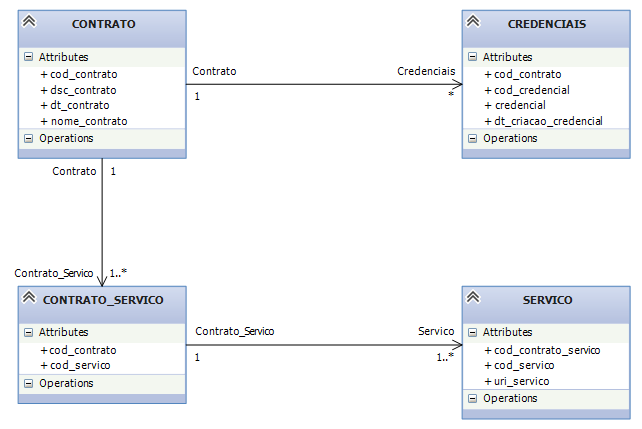
\includegraphics[width=1.0\textwidth]{modelo_relacionamento_contrato_2.png}
    \caption{Diagrama de relacionamento entre contrato, credenciais e usuários}
    \label{fig:diagrama_relacionamento}
\end{figure}


%Para a implementação de segurança em aplicações REST, verificou-se que ela passa basicamente pela aplicação de segurança em protocolos \emph{HTTP}, que oferece dois tipos de autenticação:  \emph{Basic} e \emph{Digest}.

%A autenticação Basic é um modelo baseado no desafio e resposta, sendo utilizada por servidores HTTP para validar a autenticação~\cite{franks1999}. Desta forma, quando o cliente tenta acessar algum recurso protegido, a sua identidade é requerida pelo servidor, o cliente então fornece a resposta codificada em base64 no header \emph{HTTP},  se a resposta for correta ela terá acesso ao sistema. Porém, por não criptografar o desafio, estando esse apenas codificado, faz com que ele seja vulnerável e sujeito a ataques, como por exemplo, os de repetição.

%Já na Digest, o processo é o mesmo que na autenticação básica. Sendo que seu mecanismo de autenticação é um pouco mais complexo, uma vez que ele gera um HASH, geralmente utilizando o algoritmo MD5, do desafio que será enviado pelo servidor ao cliente ~\cite{franks1999}. Apesar de ser mais seguro do que a autenticação básica, autenticação HTTP Digest também é vulnerável à ataques, como por exemplo o man-in-the-middle.  Para evitar esse problema, deve ser empregado a segurança na camada de transporte~\cite{Webber10}.

\section{Arquitetura do Protoloco}\label{sec:ArqProtocolo}

A arquitetura do protocolo proposto é apresentada na Figura~\ref{fig:arquiteturaprotocolo}. O protocolo é composto por quatro componentes: Cliente, \servidorAA, \servidorRest, e \servidorBD, que gerencia contratos, credenciais e \emph{tokens} de acesso.

\begin{figure}[!htb]
    \centering
    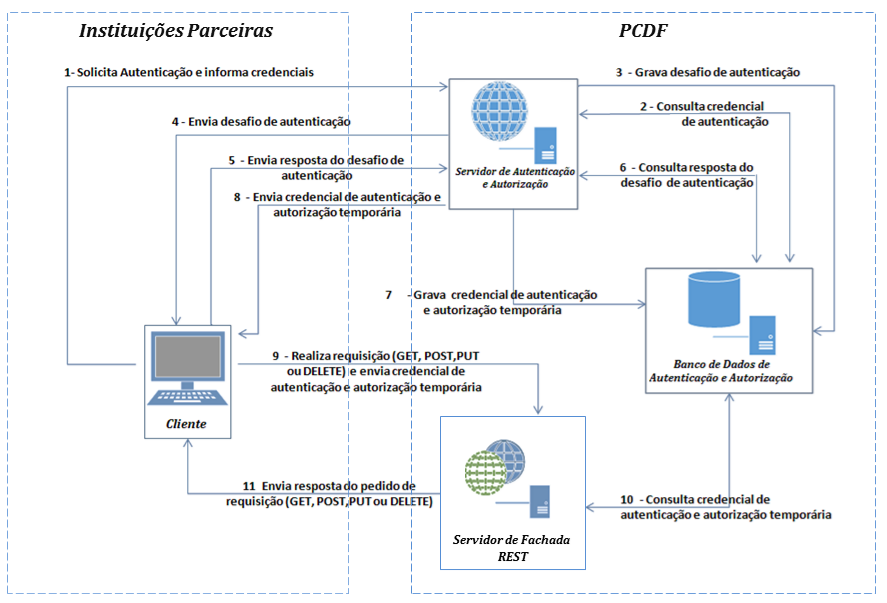
\includegraphics[width=1.0\textwidth]{arquitetura_protocolo1.png}
    \caption{Arquitetura do Protocolo de Autenticação e Autorização proposto.}
    \label{fig:arquiteturaprotocolo}
\end{figure}

O componente Cliente na arquitetura do protocolo representa as Instituições ou Órgãos conveniados, que após firmar um contrato, podem consumir os serviços ofertados pela PCDF.

O Servidor de Autenticação e Autorização tem um papel fundamental na arquitetura do protocolo, pois é neste servidor que o gerenciamento de autenticação e autorização é realizado. Desta forma, o servidor de Autenticação e Autorização é responsável por realizar os processos de verificação e validação de credenciais, criação dos desafios de autenticação, criação de \emph{tokens} JSON e a criação e o gerenciamento das credenciais de autenticação e autorização temporárias, que são utilizados pelos Clientes para consumir os serviços requisitados.

O servidor de fachada REST atua como uma fachada, abstraindo toda lógica necessária para o consumo dos serviços. Neste servidor estão concentrados os serviços REST disponibilizados pela PCDF. Desta forma, quando um Cliente necessita acessar um serviço, primeiramente ele deve ser autenticado e autorizado no servidor de Autenticação e Autorização. Após esse processo, o Cliente faz a requisição ao servidor de fachada REST, que realiza as verificações necessárias para saber se o Cliente tem privilégios ou não para acessar o serviço. O servidor de fachada REST acessa a base de dados de Autenticação e Autorização para confirmar as credenciais de autenticação e autorização temporárias informadas e, caso elas sejam válidas, permite que o Cliente acesse o serviço requerido. Um ponto importante a ser destacado é que os desenvolvedores, ao desenvolver um serviço, não necessitam ter preocupações referentes à autenticação e autorização, pois essas preocupações são de responsabilidade do servidor de fachada REST. Finalmente, o servidor de Banco de Dados mantém as informações necessárias para o funcionamento dos serviços de autenticação e autorização. É neste servidor que são salvos os usuários, os desafios e as credenciais de autorização e autenticação temporária.


\subsection{Visão Geral do Protocolo de Autenticação e Autorização Proposto}

Para ter acesso a API REST, referente aos serviços ofertados, o Cliente deve ser autenticado e autorizado a acessar o serviço. Para isso, o protocolo usa a autenticação baseada em \emph{tokens} de segurança, que são recipientes de reivindicações da autoridade emissora. Os \emph{tokens} de segurança utilizados (\emph{Web Tokens}) seguem o formato \emph{JSON}. Esse formato, ao contrário dos tokens \emph{SAML}, que são baseados em \emph{XML}, são mais compactos e, portanto, mais adequados para serem usados em um cabeçalho \emph{HTTP}. Além disso, todas as mensagens do protocolo são assinadas e criptografadas de forma assimétrica. O processo de autenticação e autorização é descrito em dois cenários distintos. No primeiro cenário, representado na Figura~\ref{fig:protocoloseguro}, o Cliente não está autenticado. No segundo cenário, o Cliente está autenticado e possui uma credencial de autorização. %Esse último é representado na figura ~\ref{fig:cenario2}.

\subsubsection{Primeiro cenário: Cliente não está autenticado}

No primeiro cenário, o Cliente não está autenticado e deve solicitar a autenticação pela primeira vez, conforme apresentado na figura~\ref{fig:protocoloseguro}

\begin{figure}[!htb]
    \centering
    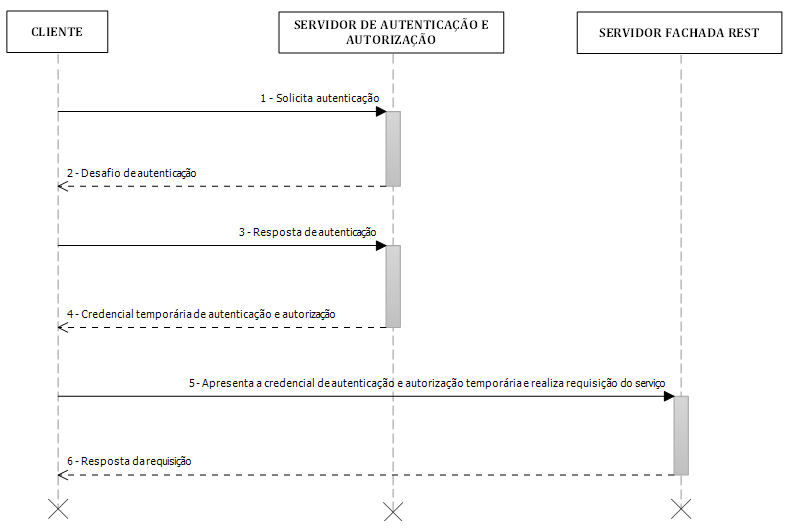
\includegraphics[width=0.9\textwidth]{fluxo_autenticacao1.png}
    \caption{Fluxo do Protocolo de Autenticação e Autorização proposto, 1º cenário.}
    \label{fig:protocoloseguro}
\end{figure}


O protocolo tem início quando o Cliente envia uma solicitação de autenticação ao \servidorAA.
Esse pedido é realizado por meio de uma mensagem (mensagem 1 da Figura~\ref{fig:protocoloseguro})que contém um \emph{token} JSON, enviado no cabeçalho HTTP da requisição REST. O \emph{token} contém uma credencial, extraída de forma aleatória da tabela de credenciais do Cliente. O \emph{token} é assinado digitalmente pelo Cliente e cifrado com a chave pública do \servidorAA. É importante frisar que tanto o Cliente quanto o \servidorAA{} possuem as mesmas tabelas de credenciais e de serviços. As tabelas são geradas no momento de assinatura do contrato de prestação do serviço.

Na segunda mensagem, "Desafio de autenticação", ao receber uma solicitação de autenticação, o \servidorAA{} extrai o \emph{token} cifrado com sua chave privada e verifica a autenticidade e integridade da requisição por meio da verificação da assinatura digital do Cliente. Se houver qualquer problema, o código HTTP 401 (usuário não autorizado) é retornada ao Cliente.
Também é feita a verificação de \emph{timestamp}, que se refere ao tempo de envio da mensagem. Caso a mensagem tenha
sido enviada em um período de tempo superior ao pré-estabelecido no contrato, o Cliente recebe como resposta o código HTTP 401 (usuário não autorizado).

Caso não ocorram problemas, procede-se com o processo de validação da credencial informada. Este processo consiste em consultar a credencial em uma base de dados e verificar se a credencial é válida e associada ao Cliente. Em seguida, o \servidorAA{} gera um desafio de autenticação. O desafio consiste em fazer uma busca aleatória à tabela de credenciais e selecionar um código de credencial que esteja associado ao Cliente. Em seguida, os dados relacionados ao desafio, a data e hora de geração do desafio e a resposta que o Cliente deverá fornecer são persistidos no \servidorBD{}. Finalmente, o \emph{token} JSON, contendo o código do desafio, o código da credencial e um \emph{timestamp} representando a data e hora de criação do desafio é enviado ao Cliente. O \emph{token} é assinado digitalmente pelo \servidorAA{} e cifrado com a chave pública do Cliente que está solicitando a autenticação.

Na terceira mensagem, "Resposta desafio de autenticação", após receber o desafio do \servidorAA{}, o Cliente extrai o \emph{token} cifrado com sua chave privada e verifica a autenticidade e integridade da requisição por meio da verificação da assinatura digital do \servidorAA{}.
Em seguida, o Cliente analisa o \emph{timestamp} com o objetivo de verificar se a mensagem foi enviada em um período de tempo superior ao pré-estabelecido no contrato. Se for detectada alguma inconsistência, o processo de autenticação atual é descartado e inicia-se um novo processo de autenticação.

Caso nenhuma inconsistência seja identificada, o Cliente verifica e responde o desafio solicitado, enviando-o
juntamente com um \emph{timestamp} e o código do serviço que deseja consumir, para o \servidorAA{} por meio de um \emph{token} JSON, que é assinado digitalmente pelo Cliente e cifrado com a chave pública do \servidorAA{}.

Na quarta mensagem, "Credencial temporária de autenticação e autorização", o \servidorAA{} recebe a resposta do desafio de autenticação, decifra o \emph{token} e verifica a autenticidade e integridade da requisição por meio da verificação da assinatura digital do Cliente. Não ocorrendo nenhuma violação, inicia-se o processo de verificação da resposta. A primeira verificação realizada refere-se ao tempo de geração do desafio, por meio do \emph{timestamp}. Se a resposta tiver sido enviada em um período de tempo superior ao pré-estabelecido em contrato, o \servidorAA{} responde com o código HTTP 401 (usuário não autorizado). Caso contrário, procede com a verificação do desafio que consiste em realizar uma consulta na tabela de desafios verificando se a resposta ao desafio corresponde a esperada. Caso a resposta esteja correta o \servidorAA{}
autentica o Cliente. Em seguida, o \servidorAA{} verifica, considerando o código do serviço requisitado, se o Cliente tem privilégios necessários para consumir o serviço requisitado.

Caso o Cliente possua os privilégios necessários, o \servidorAA{} gera uma credencial de autenticação e autorização temporária para o serviço solicitado. A credencial é gravada em uma tabela de credencias de autorização temporária, juntamente com a data e hora de criação, a data de expiração e o código do Cliente. A tabela de credencias de autorização temporária é posteriormente acessada pelo \servidorRest{} para verificar quais privilégios o Cliente tem acesso e se o mesmo está autenticado. O \emph{token}, contendo a credencial de autenticação e autorização temporária, é  assinado digitalmente pelo \servidorAA{} e cifrado  com a chave pública do Cliente. Após esse processo, o \emph{token} é enviado ao Cliente.

Caso a resposta do desafio esteja em desacordo com a esperada ou se o Cliente não tiver privilégios suficientes para acessar o serviço requisitado, a resposta do \servidorAA{} contém o código HTTP 401 (usuário não autorizado).
É importante destacar que a credencial de autenticação e autorização temporária será gerada apenas para o serviço que o Cliente tenha solicitado e possua o privilégio de acesso para utilizá-la. Nesse caso, a credencial será válida por um período  de tempo que será definido no momento da assinatura do contrato de prestação de serviço,
entre o órgão conveniado e a PCDF.

Na quinta mensagem, "Apresenta a credencial de autenticação e autorização temporária e realiza requisição do serviço", o Cliente, extrai o \emph{token} cifrado com sua chave privada e verifica a autenticidade e integridade da requisição por meio da verificação da assinatura digital do \servidorAA. Em seguida consulta o \emph{timestamp} para verificar se a mensagem foi enviada em um período de tempo superior ao pré-estabelecido no contrato. Caso ocorra alguma inconsistência, o processo de autenticação atual é descartado e inicia-se um novo processo de autenticação.

Caso não ocorram inconsistências, o Cliente verifica a data e hora de validade da credencial de autorização temporária para saber se a mesma é válida. Confirmada sua validade, o Cliente envia ao \servidorRest{}, a requisição do serviço que deseja consumir, juntamente com a credencial de autenticação e autorização temporária. O \emph{token} de autenticação e autorização temporária é assinado com a chave privada do Cliente e cifrado com chave pública do \servidorRest{}, sendo enviado no cabeçalho da requisição.

Finalmente,na sexta mensagem, "Resposta da requisição", após receber a requisição, o \servidorRest{} extrai o token cifrado com sua chave privada e verifica a autenticidade e integridade da requisição por meio da verificação da assinatura digital do \servidorAA{}. Em seguida consulta o \emph{timestamp} para checar se a mensagem foi enviada em um período de tempo superior ao pré-estabelecido no contrato. Não havendo inconsistências, o \servidorRest{} verifica se a credencial de autenticação e autorização temporária é válida. Para isso, ele realiza uma consulta na tabela de credenciais temporárias, com a finalidade de confirmar se a credencial informada não expirou, se  foi realmente gerada para o Cliente e se está associada ao serviço solicitado.

Nas situações em que a verificação é consistente, o Cliente recebe os dados referentes à sua requisição.
Havendo qualquer problema ele recebe uma resposta contendo o código HTTP 401 (usuário não autorizado).


%Já no segundo cenário, que é representado na figura ~\ref{fig:cenario2}. O Cliente, já possui uma credencial de autorização temporária, neste caso ele deverá apresentá-la sempre que desejar consumir algum serviço que ele tenha acesso.
\subsubsection{Segundo cenário: Cliente possui uma credencial de autorização temporária}

No segundo cenário, o Cliente possui uma credencial de autorização temporária,que deve ser apresentada quando requisitar algum serviço que possui acesso.
Neste caso, o Cliente envia um \emph{token} ao \servidorRest{} contendo uma credencial temporária no cabeçalho da requisição do serviço que deseja consumir. O \servidorRest{} recebe o \emph{token} de autenticação e autorização, faz a verificação na tabela de credenciais temporárias para confirmar que o Cliente possui uma credencial válida e, caso afirmativo, verifica quais são os privilégios de autorização da credencial e verifica se o Cliente possui a permissão necessária para acessar o serviço. Neste cenário, a requisição do Cliente é atendida. Por outro lado, caso a credencial não seja válida ou tenha expirado, o Cliente é redirecionado para o \servidorAA{} para que possa se autenticar novamente e obter uma nova credencial conforme descrito no primeiro cenário. Esse processo é descrito no fluxo alternativo da figura ~\ref{fig:cenario2}.

\begin{figure}[!htb]
    \centering
     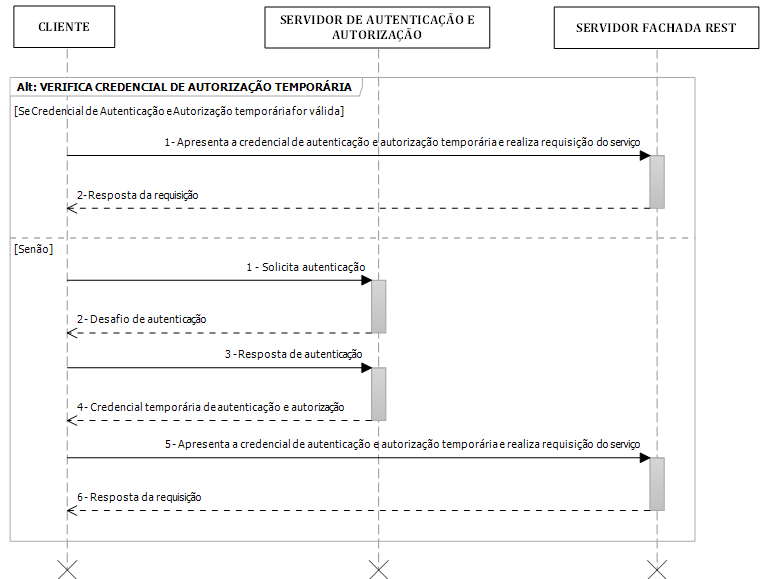
\includegraphics[width=0.8\textwidth]{cenario2_autenticacao.png}
     \caption{Fluxo do protocolo de autenticação/autorização proposto, 2º cenário.}
     \label{fig:cenario2}
\end{figure}


\section{Formalização do Protocolo}

O uso de especificações formais na área de criptografia (em particular para especificar protocolos criptográficos)
não é recente. Parte dos trabalhos nesta área foram desenvolvidos ainda na década de 90~\cite{Meadows95}, possibilitando uma análise mais detalhada dos protocolos. Com isso, o principal objetivo tem sido o de verificar se os objetivos de segurança propostos pelos autores dos protocolos criptográficos são alcançados.

Neste trabalho, o protocolo proposto foi descrito formalmente utilizando a lógica BAN, com o intuito de favorecer uma melhor comunicação e entendimento utilizando uma linguagem mais precisa. %Além disso, a propriedade de terminação com a geração da credencial temporária de autenticação e autorização foi verificada com um programa escrito em Prolog.

\subsection{Lógica BAN}

A lógica BAN foi desenvolvida por Burrows, Abadi e Needham em 1989, tendo alcançado certa popularidade para a análise de confiança e de conhecimento entre os participantes dos protocolos criptográficos~\cite{Burrows1990}. BAN é uma lógica pioneira na especificação de protocolos criptográficos, em particular protocolos usados na autenticação e
distribuição de chaves~\cite{Burrows1990}.

\subsubsection{Notação Básica}

Na lógica BAN, existem vários tipos distintos de objetos tais como entidades ou partes que se comunicam, chaves de criptografia e fórmulas lógicas. Uma fórmula lógica é uma versão idealizada da mensagem original, sendo usualmente referenciada como uma declaração lógica. Em geral, os símbolos $A$, $B$ e $S$ denotam entidades ou participantes; $Kab$, $Kas$ e $Kbs$ denotam chaves compartilhadas; $Ka$, $Kb$ e $Ks$ denotam chaves públicas e $Ka^{-1}$, $Kb^{-1}$ e $Ks^{-1}$ denotam as chaves privadas dos participantes.
Finalmente, $Na$, $Nb$ e $Ns$ são os identificadores gerados pelos participantes (referenciados como \emph{nonces}
na literatura). As construções usadas com maior frequência são apresentadas na Tabela~\ref{tab:notacaobasicaBAN}:

\newcommand{\RHQuery}{\textbf{[???]}}
\newcommand{\RHRemark}[1]{\textbf{[#1]}}
\newcommand{\Believess}[2]{{#1}\mathrel{\textbf{\mid\equiv}}{#2}}
\newcommand{\Seess}[2]{{#1}\mathrel{\textbf{\triangleleft}}{#2}}
\newcommand{\Saids}[2]{{#1}\mathrel{\textbf{\mid\sim}}{#2}}

\newcommand{\Believes}[2]{{#1}\mathrel{\textbf{acredita}}{#2}}
\newcommand{\Sees}[2]{{#1}\mathrel{\textbf{recebeu}}{#2}}
\newcommand{\Said}[2]{{#1}\mathrel{\textbf{disse}}{#2}}
\newcommand{\Controls}[2]{{#1}\mathrel{\textbf{controla}}{#2}}
\newcommand{\Fresh}[1]{{#1}\,\textbf{novo}}
\newcommand{\Share}[3]{{#1}\stackrel{#2}{\longleftrightarrow}{#3}}
\newcommand{\ShareSecret}[3]{{#1}\stackrel{#2}{\rightleftharpoons}{#3}}
\newcommand{\PubKey}[2]{{}\stackrel{#1}{\mapsto}{#2}}
\newcommand{\Secret}[3]{{#1}\stackrel{#2}{\leftrightharpoons}{#3}}
\newcommand{\Encrypt}[2]{\{\,{#1}\,\}_{#2}}
\newcommand{\EncryptFrom}[3]{\{\,{#1}\,\}_{#2}^{#3}}
\newcommand{\Attach}[2]{\langle {#1}\rangle_{#2}}

%\begin{tabular}{cp{20cm}}
\begin{table}[h]
\begin{center}
    \begin{tabular}{|l|p{12cm}|}
    \hline
    \textbf{\emph{Expressão }}         & \textbf{\emph{Leitura/Significado}}                                                                               \\ \hline
    ${P}\mid\equiv{X}$               & $\Believes{P}{X}$: $P$ confia em $X$, ou $P$ acredita que $X$ é verdadeiro. \\ \hline

    ${P}\triangleleft{X}$            & $\Sees{P}{X}$: Alguém enviou uma mensagem para $P$ contendo $X$; ou seja, $P$ recebeu $X$.   \\ \hline

     ${P}\mid\sim{X}$                 & $\Said{P}{X}$: $P$ alguma vez compartilhou $X$. Pode-se assumir que a entidade $P$
        em algum momento enviou uma mensagem incluíndo a declaração $X$.\\ \hline

    ${P}\Rightarrow {X}$                 & $\Controls{P}{X}$: $P$ tem jurisdição sobre $X$, onde $P$ é uma autoridade sobre $X$ e deve ser confiável. \\ \hline

    \#(X)                            & novo$(X)$: a fórmula $X$ não foi usada em mensagens anteriores à execução atual do protocolo.  \\ \hline

    $\Share{P}{k}{Q}$                & (lê-se ``k é uma chave satisfatória para $P$ e $Q$''). A chave $k$ n\~{a}o pode ser descoberta
                                             por qualquer outro participante, exceto $P$, $Q$ ou por alguém que ambos confiam. \\ \hline

    $\{{X}\}_K$                  & fórmula $X$ foi cifrada com a chave $K$. As mensagens cifradas são legíveis e verificáveis apenas pelos
                                       participantes que conhecem a chave $K$. \\ \hline

    $\ShareSecret{P}{k}{Q}$         & ${k}$ é um segredo compartilhado entre ${P}$ e ${Q}$ e possivelmente as entidades de confiança de $P$ e $Q$.
                                                 Somente ${P}$ e ${Q}$ podem usar $k$ para provar suas identidades. \\ \hline

    $\PubKey{K}{P}$:               & ${k}$ é a chave pública de ${P}$.  \\ \hline
    \end{tabular}
    \caption {Notação básica da Lógica BAN, adaptação de ~\cite{Burrows1990}.}
\label{tab:notacaobasicaBAN}
\end{center}
\end{table}


\subsubsection{Postulados Lógicos}

No estudo de protocolos de segurança é importante diferenciar o tempo das demonstrações ou eventos. Caso isso não seja observado, problemas como a não detecção do reenvio de mensagens podem ocorrer. Dessa forma, a lógica BAN trata dessa distinção dividindo-a em duas épocas: presente, que é o tempo durante a execução do protocolo, e o passado, que refere-se às mensagens enviadas antes da execução do protocolo, o que faz com que elas sejam rejeitadas, uma vez que não são confiáveis~\cite{Burrows1990}. Essa divisão de tempo é suficiente para facilitar o entendimento sobre como a lógica pode ser manipulada. Para realizar a análise dos protocolos de segurança, a lógica BAN possui uma série de postulados lógicos. No restante dessa seção apresentamos alguns desses postulados, reforçando que maiores detalhes podem ser encontrados no artigo que introduziu a notação BAN~\cite{Burrows1990}

\begin{enumerate}[(P1)]

 \item Regra de significado da mensagem. Esta regra faz parte da interpretação das mensagens. Para as chaves secretas compartilhadas, temos que:

    \begin{displaymath}
        \infer
        {{P}\mid\equiv{{Q}\mid\sim{X}}}
        {{P}\mid\equiv{\Share{P}{k}{Q}}& {P}\triangleleft{\Encrypt{X}{k}}}
        %{\Believes{P}{\Said{Q}{X}}}
        %{\Believes{P}{\Share{P}{k}{Q,}}&\Sees{P}{\Encrypt{X}{k}}}
    \end{displaymath}

Ou seja, assumindo que $P$ acredita que $k$ é uma chave satisfatória para se comunicar com $Q$, e que
$P$ recebeu a mensagem $X$ cifrada com a chave $k$, então $P$ acredita que $Q$ uma vez disse $X$.
De forma similar, esse postulado quando consideramos chaves públicas estabelece que:

    \begin{displaymath}
        \infer
        {{P}\mid\equiv{{Q}\mid\sim{X}}}
        {{P}\mid\equiv{\PubKey{K}{Q}}& {P}\triangleleft{\Encrypt{X}{k ^{-1}}}}
                %{\Believes{P}{\Said{Q}{X}}}
                %{\Believes{P}{\Share{P}{k}{Q,}}&\Sees{P}{\Encrypt{X}{k}}}
    \end{displaymath}


\item Regra de verificação do identificador. Essa regra estabelece que, dada uma mensagem recente, enviada durante a execução atual do protocolo é possível assumir que o emissor confia na mensagem.

  \begin{displaymath}
    \infer
    {{P}\mid\equiv{{Q}\mid\equiv{X}}}
    {{P}\mid\equiv{\#(X),}& {P}\mid\equiv{{Q}\mid\sim{X}}}
    %{\Believes{P}{\Believes{Q}{X}}}
    %{\Believes{P} novo$(X),$ &\Believes{P}{\Said{Q}{X}}}
  \end{displaymath}

   Se $P$ acredita que $X$ é novo e $P$ acredita que em algum momento $Q$ disse $X$, então $P$ assume que $Q$ confia em X.

\item Regra da jurisdição. Esta regra representa a confiança e a autoridade de uma entidade sobre as declarações.
\begin{displaymath}
    \infer
    {{P}\mid\equiv{X}}
    {{P}\mid\equiv{{Q}\Rightarrow {X},}& {P}\mid\equiv{{Q}\mid\equiv{X}}}
   % {\Believes{P}{X}}
   % {\Believes{P}{\Controls{Q}{X},} &\Believes{P}{\Believes{Q}{X}}}
  \end{displaymath}

   Se $P$  acredita que $Q$ tem jurisdição sobre a declaração $X$ e $P$ acredita que $Q$ acredita em $X$, então $P$ confia na declaração $X$.

\end{enumerate}

Estes são os postulados fundamentais na análise formal do protocolo criptográfico proposto nessa dissertação.
A utilização destas regras, juntamente com as notações descritas na sessão anterior, possibilita o estabelecimento da confiança entre os participantes de um protocolo.

\subsection{Análise Formal do Protocolo Proposto}

Nesta sessão apresentamos a análise formal do protocolo de autenticação e autorização proposto, seguindo o processo
descrito em~\cite{Burrows1990}. De acordo com o referido processo, a análise de um protocolo é realizada em quatro etapas, que serviram para organizar o restante dessa seção.

\subsubsection{Idealização do protocolo}

\newcommand{\HT}[3]{\{\,{#1}\,\}\,{#2}\,\{\,{#3}\,\}}
\newcommand{\Msg}[3]{{#1}\longrightarrow{#2}:\,{#3}}

Para especificar o protocolo formalmente, foram utilizadas algumas notações para representar os elementos participantes. Logo, os símbolos ${A}$, ${B}$ e ${C}$ são utilizadas para representar respectivamente as entidades que trocam mensagens entre si. No protocolo proposto, temos como participantes os nós Cliente, \servidorRest{} e
\servidorAA. As chaves públicas das entidades ${A}$, ${B}$ e ${C}$ são representadas, respectivamente, por ${Ka}$, ${Kb}$ e ${Kc}$. As chaves privadas, seguindo o mesmo pressuposto, são representadas pelos símbolos ${{Ka}^{-1}}$, ${{Kb} ^{-1}}$ e ${{Kc} ^{-1}}$. Os elementos ${Cred_A}$ e ${Cod_{Srv_A}}$ representam, respectivamente,
a credencial utilizada pela entidade ${A}$ e o código que identifica o serviço que a entidade ${A}$ deseja consumir.

O desafio, gerado pela entidade ${C}$ e enviado a entidade ${A}$, \'{e} representado pela fórmula ${N_{CA}}$. Essa f\'{o}rmula contempla o código do desafio gerado pela entidade ${C}$ e o código da credencial aleatória da entidade ${A}$. A resposta do desafio gerado pela entidade ${C}$ e enviada à entidade ${A}$ é representada pela f\'{o}rmula ${Resp_{AC}}$. Essa f\'{o}rmula corresponde ao código do desafio gerado pela entidade ${C}$ e a credencial solicitada pela entidade ${A}$. ${Ts_A}$ e ${Ts_C}$ são, respectivamente, os \emph{timestamps} emitidos pelas entidades ${A}$ e ${C}$.

O símbolo ${Msg_{AC}}$ representa o resumo da mensagem enviada pela entidade ${A}$ à entidade ${C}$, ${Msg_{CA}}$ representa o resumo da mensagem enviada pela entidade ${C}$ à entidade ${A}$ e ${Msg_{AB}}$ representa o resumo da mensagem enviada pela entidade ${A}$ à entidade ${B}$. O elemento ${H}$ representa a aplicação de uma função \emph{Hash} a uma mensagem.
Finalmente, o símbolo ${Exp_A}$ representa a data/hora  de expiração da credencial temporária de autorização e autenticação, ${C_{Aut}}$ corresponde à credencial temporária de autorização e autenticação gerada para a entidade A e ${Req_A}$ refere-se à requisição de serviços realizadas a partir da entidade $A$, utilizando algum dos métodos do protocolo HTTP (GET, PUT, POST ou DELETE).

Para especificar formalmente um protocolo de segurança utilizando a lógica BAN, é necessário idealizar o protocolo e, a partir da aplicação dos postulados e das suposições iniciais, verificar se ele atinge ou não o seu objetivo. A idealização do protocolo proposto é descrito na figura~\ref{fig:protocoidealizado}, representando o fluxo de troca de mensagens executado pelo protocolo. % {\color{blue}n\~{a}o entendi: Todas as mensagens são consideradas na análise, pois utilizam criptografia assimétrica desde a primeira troca de mensagens}.

\begin{figure}[!htb]
    \centering
    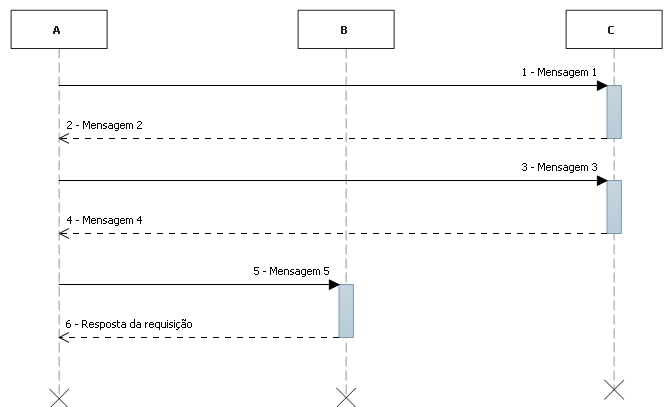
\includegraphics[width=0.8\textwidth]{fluxo_autenticacao_BAN.png}
    \caption{Diagrama com a idealização do protocolo de autenticação/autorização proposto}
    \label{fig:protocoidealizado}
\end{figure}

\begin{enumerate}
  \item Mensagem 1: $\Msg{A}{C}{\Encrypt{Ts_A,Cred_A,H{\Encrypt{Msg_{AC}}{Ka ^{-1}}}}{Kc}}$.
  \item Mensagem 2: $\Msg{C}{A}{\Encrypt{Ts_C,{N_{CA}},H{\Encrypt{Msg_{CA}}{Kc ^{-1}}}}{Ka}}$.
  \item Mensagem 3: $\Msg{A}{C}{\Encrypt{Ts_A,{Resp_{AC}},Cod_{Srv_A},H{\Encrypt{Msg_{AC}}{Ka ^{-1}}}}{Kc}}$.
  \item Mensagem 4: $\Msg{C}{A}{\Encrypt{Ts_C,Exp_A,\#(\ShareSecret{A}{{C_{Aut}}}{C}),H{\Encrypt{Msg_{CA}}{Kc ^{-1}}}}{Ka}}$.
  \item Mensagem 5: $\Msg{A}{B}{\Encrypt{Ts_A,(\ShareSecret{A}{{C_{Aut}}}{C}),H{\Encrypt{Msg_{AB}}{Ka ^{-1}}}}{Ka}},{Req_A}$.

  %{\color{blue}\item Mensagem 5: $\Msg{A}{B}{\Encrypt{Ts_A,(\ShareSecret{A}{{C_{Aut}}}{C}),H{\Encrypt{Msg_{AB}}{Ka ^{-1}}}}{Ka}},{Req_A}$.}\footnote{V\'{a}rias d\'{u}vidas. Por que enviar $Req_A$? Por que essa mensagem para B?}
\end{enumerate}

\subsubsection{Suposições}\label{sec:Suposicoes}

O objetivo do protocolo é fazer com que a entidade ${A}$ seja autenticada pela entidade ${C}$ e obtenha uma credencial de autenticação e autorização temporária, referente a uma requisição de um serviço que a entidade ${A}$ deseja consumir. Com isso, a credencial de autenticação e autorização temporária pode ser utilizada pela entidade ${A}$ no momento da requisição do serviço à entidade ${B}$ e, assim, realizar a computação que deseja via o consumo a um serviço de forma segura. Para isso, algumas suposições iniciais são estabelecidas e, juntamente com a aplicação dos postulados da lógica BAN, busca-se verificar se o protocolo alcança o objetivo proposto. Todas as suposições, apresentadas na Tabela~\ref{tab:suposicoesBAN}, são baseadas no uso de um canal seguro de comunicação SSL/TSL. %; onde tanto o receptor  quanto o emissor do serviço são conhecidos e autenticados {\color{blue}isso eh necess\'{a}rio indicar?} com o uso de certificados digitais X.509.

\begin{table}[h]
\begin{tabular}{cllcl}
\textbf{Suposição} & \textbf{Descrição} &  & \textbf{Suposição} & \textbf{Descrição} \\
\textbf{1 -}       & $ A \mid\equiv$  ${\PubKey{Kc}{C}}$                 &  & \textbf{9 -}       & $ B \mid\equiv$ $ C \Rightarrow $ $\#(\ShareSecret{A}{{C_{Aut}}}{C})$ \\
\textbf{2 -}       & $ B \mid\equiv$  ${\PubKey{Ka}{A}}$                 &  & \textbf{10 -}      & $ A \mid\equiv$ $ C \mid\equiv $ $\#(\ShareSecret{A}{{C_{Aut}}}{C})$ \\
\textbf{3 -}       & $ C \mid\equiv$  ${\PubKey{Ka}{A}}$                 &  & \textbf{11 -}      & $ B \mid\equiv$ $ C \mid\equiv $ $\#(\ShareSecret{A}{{C_{Aut}}}{C})$ \\

\textbf{4 -}       & $ A \mid\equiv$  $\#{Ts_C}$                         &  & \textbf{12 -}      & $ A \mid\equiv$  $\#(\ShareSecret{A}{{C_{Aut}}}{C})$  \\

\textbf{5 -}       & $ B \mid\equiv$  $\#{Ts_A}$                         &  & \textbf{13 - }      & $ B \mid\equiv$  $\#(\ShareSecret{A}{{C_{Aut}}}{C})$  \\

\textbf{6 -}       & $ C \mid\equiv$  $\#{Ts_A}$                         &  & \textbf{ }                    &                                      \\
\textbf{7 -}       & $ A \mid\equiv$  ${Exp_A}$                          &  & \textbf{ }                   &
\\
\textbf{8 -}       & $ A \mid\equiv$  $ C \Rightarrow $ $\#(\ShareSecret{A}{{C_{Aut}}}{C})$   &   & \textbf{ }     &                               \\
\end{tabular}
\caption {Suposições aplicadas ao protocolo proposto.}
\label{tab:suposicoesBAN}
\end{table}


Dessa forma, temos que as suposições 1, 2 e 3 garantem que as entidades participantes ${A}$, ${B}$ e ${C}$ confiam  nas chaves públicas das entidades que farão as trocas de mensagem. As suposições 4, 5 e 6 são \emph{timestamps}, o que denota que as entidades ${A}$, ${B}$ e ${C}$ devem estar sincronizadas. Sendo assim, a entidade ${A}$ acredita que o \emph{timestamp} ${Ts_C}$ é novo e foi gerado recentemente. Da mesma forma que as entidades ${B}$ e ${C}$ acreditam  que o \emph{timestamp} ${Ts_A}$ também é novo e foi gerado recentemente. A suposição 7 é utilizada pela entidade ${A}$ para garantir que a credencial de autenticação e autorização gerado pela entidade ${C}$ não expirou e que pode ser utilizada. As suposições 8 e 9 denotam que as entidades ${A}$ e ${B}$ acreditam que entidade ${C}$ tem jurisdição  sobre a credencial de autenticação e autorização gerada. Portanto, as suposições 10 e 11 garantem que as entidades ${A}$, ${B}$ acreditam que a credencial de autenticação e autorização gerada é nova é foi realmente gerada pela entidade ${C}$. Finalmente, as suposições 12 e 13 garantem que as entidades ${A}$ e ${B}$ acreditam na nova credencial de autenticação e autorização temporária representada por ${C_{Aut}}$.

\subsubsection{Provas}

Como o objetivo final do protocolo é autenticar a entidade ${A}$, de forma que ela obtenha uma credencial de autenticação e autorização temporária e referente a uma requisição de serviço desejado. Nessa seção, será realizada uma análise de cada mensagem do protocolo idealizado, aplicando os postulados lógicos e suposições com o intuito de provar que o protocolo consegue atingir o objetivo proposto.

Na primeira mensagem, a entidade ${A}$ envia sua credencial, um \emph{timestamp} e o código do serviço que ele está querendo consumir ao \servidorAA,
representado pela entidade ${C}$. A mensagem enviada é assinada com a chave privada do participante ${A}$  e cifrada com a chave pública do participante ${C}$.
Ap\'{o}s o recebimento dessa mensagem, o estado da execu\c c\~{a}o do protocolo evolui conforme a descri\c c\~{a}o.

\textbf{Mensagem 1}: $\Msg{A}{C}{\Encrypt{Ts_A,Cred_A,H{\Encrypt{Msg_{AC}}{Ka ^{-1}}}}{Kc}}$.

$C\triangleleft$ ${\Encrypt{Ts_A,Cred_A,Cod_{Srv_A},H{\Encrypt{Msg_{AC}}{Ka ^{-1}}}}{Kc}}$

$C\mid\equiv A \mid\sim $  $H\{Msg_{AC}\}$

$C\mid\equiv A \mid\sim$ ${\#Ts_A}$

$C\mid\equiv$ ${Cred_A,Cod_{Srv_A}}$

Dessa forma, $C$ recebe a fórmula ${\Encrypt{Ts_A,Cred_A,Cod_{Srv_A},H{\Encrypt{Msg_{AC}}{Ka ^{-1}}}}{Kc}}$ e, usando sua chave privada, decifra a fórmula recebida.
Após decifrar a fórmula, e aplicando a regra do significado da mensagem na suposição 3 e usando a função $H \{Msg_{AC}\}$ confirma a autenticidade e integridade da mensagem.
Por fim, aplica a regra de verificação do identificador na suposição 6 usando a fórmula ${Ts_A}$ para obter a credencial da entidade ${A}$ (identificada pela fórmula ${Cred_A}$).

Na segunda mensagem, após receber e validar os dados enviados por $A$, a entidade ${C}$ gera um desafio de autenticação, ${N_{CA}}$. O desafio consiste em fazer uma busca aleatória à tabela de credenciais e selecionar um código de credencial que esteja associado \`{a} entidade $A$. Em seguida grava-se o desafio, a data e hora de geração do desafio e a resposta esperada em uma base de dados. Na sequência, uma mensagem \'{e} enviada uma mensagem \'{a} entidade $A$. A mensagem, que contém o desafio e um \emph{timestamp}, precisa ser assinada com a chave privada da entidade ${C}$ e cifrada com a chave pública da entidade ${A}$.
Logo, temos que:

\textbf{Mensagem 2}: $\Msg{C}{A}{\Encrypt{Ts_C,{N_{CA}},H{\Encrypt{Msg_{CA}}{Kc ^{-1}}}}{Ka}}$.

$A \triangleleft$ ${\Encrypt{Ts_C,{N_{CA}},H{\Encrypt{Msg_{CA}}{Kc ^{-1}}}}{Ka}}$

$A \mid\equiv C \mid\sim $  $H \{Msg_{CA}\}$

$A \mid\equiv C \mid\sim$ ${Ts_C}$

$A \mid\equiv$ ${N_{CA}}$

A entidade $A$ recebe a fórmula ${\Encrypt{Ts_C,{N_{CA}},H{\Encrypt{Msg_{CA}}{Kc ^{-1}}}}{Ka}}$ e a decifra usando sua chave privada. Em seguida, aplicando a regra do significado da mensagem na suposição 1 usando a função $H \{Msg_{CA}\}$, confirma a autenticidade e integridade da mensagem. Por fim, aplica a regra de verificação do identificador na suposição 4, usando a fórmula ${Ts_C}$ para obter o desafio ${N_{CA}}$ gerado pela entidade ${C}$. Como resultado, ${A}$ obtém  o desafio de autenticação gerado pela entidade ${C}$.

Na terceira mensagem, a entidade ${A}$, após receber e validar o desafio gerado pela entidade ${C}$, envia a resposta ${Resp_{AC}}$, conforme solicitado. Essa resposta consiste em informar o código do desafio gerado pela entidade ${C}$ e a credencial associada ao código de credencial solicitada pela entidade ${C}$. Além disso, a entidade ${A}$ deve informar o código do serviço que deseja consumir. Dessa forma, temos:

\textbf{Mensagem 3}: $\Msg{A}{C}{\Encrypt{Ts_A,{Resp_{AC}},Cod_{Srv_A},H{\Encrypt{Msg_{AC}}{Ka ^{-1}}}}{Kc}}$.

$C\triangleleft$ ${\Encrypt{Ts_A,{Resp_{AC}},H{\Encrypt{Msg_{AC}}{Ka ^{-1}}}}{Kc}}$

$C\mid\equiv A \mid\sim $  $H \{Msg_{AC}\}$

$C\mid\equiv A \mid\sim$ ${\#Ts_A}$

$C\mid\equiv$ ${Resp_{AC}}$

A entidade $C$ recebe a fórmula ${\Encrypt{Ts_A,{Resp_{AC}},H{\Encrypt{Msg_{AC}}{Ka ^{-1}}}}{Kc}}$ e a decifra usando sua chave privada. Em seguida, aplicando a regra do significado da mensagem na suposição 3 e usando a função $H \{Msg_{AC}\}$, confirma a autenticidade e integridade da mensagem. Por fim, aplica a regra de verificação do identificador na suposição 6 usando a fórmula ${Ts_A}$ para obter os dados da resposta do desafio ${Resp_{AC}}$. Com isso, é possível validar a resposta enviada e autenticar a entidade ${A}$, dando início ao processo de autorização. Como resultado temos que a entidade ${C}$ autentica a entidade ${A}$.

Na mensagem 4, após autenticar a entidade ${A}$, a entidade ${C}$ procede com o processo de autorização, que consiste em verificar qual serviço a entidade está querendo consumir. Para isso, a entidade C verifica o código de serviço solicitado pela entidade ${A}$, $Cod_{Srv_A}$, que foi informado no envio da mensagem 3. Se a entidade ${A}$ possuir os privilégios necessários para consumir o serviço requisitado, a entidade ${C}$ gera uma nova credencial de autorização temporária para o serviço solicitado. Em seguida, a entidade ${C}$ grava a credencial ${(\ShareSecret{A}{{C_{Aut}}}{C})}$, o código do serviço que a entidade ${A}$ está requerendo, a data e hora de criação, a data de expiração e o código do contrato da entidade ${A}$. Terminado esse procedimento, a entidade ${C}$, envia uma mensagem contendo a credencial ${(\ShareSecret{A}{{C_{Aut}}}{C})}$, a data e hora de expiração da credencial (${Exp_A}$) e um \emph{timestamp} a entidade ${A}$. Esta mensagem é assinada com a chave privada da entidade ${C}$ e cifrada com a chave pública da entidade ${A}$.


\textbf{Mensagem 4}: $\Msg{C}{A}{\Encrypt{Ts_C,Exp_A,\#(\ShareSecret{A}{{C_{Aut}}}{C}),H{\Encrypt{Msg_{CA}}{Kc ^{-1}}}}{Ka}}$.

$A \triangleleft$ $\Msg{C}{A}{\Encrypt{Ts_C,Exp_A,\#(\ShareSecret{A}{{C_{Aut}}}{C}),H{\Encrypt{Msg_{CA}}{Kc ^{-1}}}}{Ka}}$.

$A \mid\equiv C \mid\sim $  $H \{Msg_{CA}\}$

$ A \mid\equiv C \mid\sim$ ${Ts_C}$

$A \mid\equiv C \mid\sim$ ${Exp_A}$

$A \mid\equiv C \Rightarrow $  ${\#(\ShareSecret{A}{{C_{Aut}}}{C})}$

$A \mid\equiv C \mid\equiv $  ${\#(\ShareSecret{A}{{C_{Aut}}}{C})}$

$A \mid\equiv$ ${\#(\ShareSecret{A}{{C_{Aut}}}{C})}$

A entidade ${A}$ recebe a fórmula ${\Encrypt{Ts_C,Exp_A,\#(\ShareSecret{A}{{C_{Aut}}}{C}),H{\Encrypt{Msg_{CA}}{Kc ^{-1}}}}{Ka}}$ e a decifra usando sua chave privada. Em seguida, aplicando a regra do significado da mensagem na suposição 1 e usando a função $H \{Msg_{CA}\}$, confirma a autenticidade e integridade da mensagem. A entidade $A$
aplica a regra de verificação do identificador nas suposições 4 e 7 usando as fórmulas ${Ts_C}$  e ${Exp_A}$. E, finalmente, aplicando a regra da jurisdição, nas suposições 7 e 9, obtém a credencial de autorização temporária ${\#(\ShareSecret{A}{{C_{Aut}}}{C})}$.

Finalmente, na quinta mensagem, a entidade ${A}$ após receber e validar a mensagem enviada pela entidade ${C}$, obtendo assim a credencial de autenticação e autorização temporária, ${\#(\ShareSecret{A}{{C_{Aut}}}{C})}$, envia uma mensagem à entidade ${B}$ contendo a requisição do serviço que deseja consumir juntamente com a credencial de autorização temporária. Esta mensagem é assinada com a chave privada da entidade ${A}$ e cifrada com a chave pública da entidade ${B}$.

\textbf{Mensagem 5}: $\Msg{A}{B}{\Encrypt{Ts_A,(\ShareSecret{A}{{C_{Aut}}}{C}),H{\Encrypt{Msg_{AB}}{Ka ^{-1}}}}{Kb}},{Req_A}$.

$B\triangleleft$  ${\Encrypt{Ts_A,(\ShareSecret{A}{{C_{Aut}}}{C}),H{\Encrypt{Msg_{AB}}{Ka ^{-1}}}}{Kb}},{Req_A}$

$B\mid\equiv A \mid\sim $  $H\{Msg_{AB}\}$

$B\mid\equiv A \mid\sim$ ${Ts_A}$

$B\mid\equiv A \Rightarrow $  ${\#(\ShareSecret{A}{{C_{Aut}}}{C})}$

$B\mid\equiv A \mid\equiv $  ${\#(\ShareSecret{A}{{C_{Aut}}}{C})}$

$B\mid\equiv$ ${\#(\ShareSecret{A}{{C_{Aut}}}{C})}$

Como resultado, a entidade $B$ recebe a fórmula ${\Encrypt{Ts_A,(\ShareSecret{A}{{C_{Aut}}}{C}),H{\Encrypt{Msg_{AB}}{Ka ^{-1}}}}{Kb}},{Req_A}$, e a decifra, usando sua chave privada. Em seguida, aplicando a regra do significado da mensagem na suposição 2 e usando a função $H\{Msg_{AB}\}$, confirma a autenticidade e integridade da mensagem. A entidade $B$ aplica a regra de verificação do identificador na suposições 5 usando as fórmulas ${Ts_A}$. Finalmente, aplicando a regra da jurisdição nas suposições 8 e 10, obtém a credencial de autorização temporária ${\#(\ShareSecret{A}{{C_{Aut}}}{C})}$ e autoriza a entidade A a consumir a requisição ${Req_A}$. Como resultado, ${B}$ autoriza ${A}$, a partir da nova credencial ${(\ShareSecret{A}{{C_{Aut}}}{C})}$, a consumir a requisição ${Req_A}$

\subsubsection{Análise}

A análise demonstra que o protocolo de autenticação e autorização proposto alcança os objetivos apresentados--- ou seja, a autenticação da entidade ${A}$ e a emissão da credencial de autenticação e autorização temporária. Isso permite que a entidade ${A}$ consuma o serviço requerido. É importante frisar que a lógica BAN foi utilizada para (a) comunicar de forma mais precisa a execução do protocolo e (b) permitir uma verificação mais precisa sobre possíveis falhas no protocolo. %{\color{blue}precisamos discutir isso, pois voc\^{e} apresenta uma an\'{a}lise de seguran\c ca no pr\'{o}ximo cap\'{i}tulo} Para verificar a segurança do protocolo é necessário que seja empregado um método de criptoanálise sobre a criptografia utilizada e assim verificar quais são vulnerabilidades que o protocolo ou os algoritmos criptográficos empregados estão sujeitos.


\section{Implementação}\label{sec:implementacao}

Após a definição do protocolo proposto, e para atender o interesse na realização de testes de desempenho que objetivam avaliar o impacto da solução, foi feita a implementação de um protótipo para o protocolo de autenticação e autorização. Esse protótipo foi desenvolvido em conjunto com um trabalho de conclussão de curso do aluno Alexandre Lucchesi (da Engenharia da Computação, UnB).

\subsection{Protótipo}

Para implementar o protótipo do protocolo proposto foi necessário desenvolver cada um dos componentes (Cliente, \servidorAA e \servidorRest) descritos na arquitetura do protocolo na seção~\ref{sec:ArqProtocolo}. Para isso, foi utilizada a linguagem de programação funcional Haskell, com o compilador GHC (Glasgow Haskell Compiler).
Para o controle de dependências e gerenciamento de \emph{build} de aplicações foi utilizada a ferramenta Cabal, que é um gerenciador de pacotes do Haskell. Com ele é possível construir aplicações e bibliotecas de forma padronizada, organizada e portável. Para criar o protótipo ainda foi utilizado o framework Haskell para desenvolvimento web, denominado Snap \emph{Framework} que é necessário para lidar com as requisições HTTP. Estas requisições são utilizadas pelo protocolo de autenticação e autorização proposto. Além disso, foi utilizado o HsOpenSSL que é um OpenSSL vinculativo para Haskell, utilizado para garantir a utilização do HTTPS em todas as trocas de mensagem a partir de código Haskell.

Para a assinatura digital das mensagens utilizadas pelo protocolo foi utilizado o algoritmo RSASSA\-PKCS\-v1\_5 SHA\-256 conforme orientação descrita na publicação~\cite{ietfjws} e para criptografia foi utilizado o algoritmo de criptografia assimétrica, RSAES\-PKCS1\-V1\_5, para cifrar a chave simétrica utilizada no algoritmo de criptografia simétrica AES\_128\_CBC\_HMAC\_SHA\_256 que foi utilizado para cifrar a mensagem. Procurou-se seguir a orientação do que é preconizado na publicação~\cite{jwt2014}.

O servidor de banco de dados foi implementado utilizando o banco de dados não relacional \emph{Apache CouchDB}, que é um banco de dados flexível e tolerante a falhas que usa \emph{JSON} para armazenar os dados e JavaScript como sua linguagem de consulta usando o MapReduce. Além disso, o \emph{Apache CouchDB} oferece uma API de acesso de acordo com o estilo REST.

O protótipo implementado não objetivou a otimização de código. Seu objetivo foi o de possibilitar a realização dos testes de desempenho em uma configuração mais rudimentar em termos de desempenho, o que leva a possibilidades de melhoria em relação ao processamento das requisições. Além disso, o protótipo permitiu verificar as funcionalidades do protocolo proposto.


\section{Síntese do Capítulo}

Este capítulo apresentou os requisitos e a arquitetura do protocolo de autenticação e autorização proposto. Além disso, o capítulo apresentou a formalização do protocolo utilizando à lógica BAN. Finalmente, foi apresentada de forma sucinta a implementação de um protótipo para protocolo proposto. No próximo capítulo fazemos uma análise de segurança do protocolo proposto (conforme o trabalho apresentado em~\cite{traust08}) e apresentamos uma análise de desempenho a fim de mensurar o impacto da adoção protocolo de autenticação e autorização proposto. %na infraestrutura da PCDF. 
  \chapter{Avaliação e análise de desempenho}

Com a definição da arquitetura de referência \emph{REST}  e do protocolo de autenticação e autorização (Capítulo~\ref{cap:Protocolo}), 
tornou-se necess\'{a}ria a realiza\c c\~{a}o de uma an\'{a}lise de seguran\c ca e de experimentos que possibilitam a mensuração do 
impacto da sua utilização no tratamento das requisi\c c\~{o}es realizadas \`{a} PCDF. Neste caso, procedemos com 
a investiga\c c\~{a}o das seguintes quest\~{o}es

\parbox{0.8\textwidth}{
\begin{enumerate}[(Q1)]
\item \emph{Qual o impacto observado no tempo de resposta às requisi\c c\~{o}es com o uso do protocolo?}
\item \emph{Um prot\'{o}tipo funcional, sem foco em otimiza\c c\~{a}o, consegue suportar a demanda prevista?}
\end{enumerate}}


Este capítulo inicialmente apresenta uma an\'{a}lise dos mecanismos de seguran\c ca propostos no protocolo. Essa primeira 
an\'{a}lise segue um procedimento informal, mas est\'{a} de acordo com trabalhos descritos na literatura~\cite{} {\color{red}citar 
disserta\c c\~{o}es, teses e artigos que fazem uma an\'{a}lise similar.}. Em seguida, este cap\'{i}tulo apresenta uma avalia\c c\~{a}o 
emp\'{i}rica que busca responder as quest\~{o}es enumeradas anteriormente. 

\section{Análise de Segurança}

Nesta seção serão discutidas as propriedades de segurança do protocolo de autenticação e autorização proposto. São abordadas as propriedades e alguns ataques que podem ser realizados. Essa seção segue a estrutura e se fundamenta (parcialmente) no discurso utilizado na an\'{a}lise do protocolo Traust~\cite{traust08}.

\subsection{Segurança da sessão}

O protocolo de Autenticação e Autorização proposto utiliza para segurança de {\color{red}seção} e camada de transporte, o protocolo 
TLS/SSL. A utilização desse protocolo tem por objetivo evitar o ataque \emph{man-in-the-middle}. Para isso, é exigido, tanto para o órgão conveniado quanto para a própria 
PCDF, a utiliza\c c\~{a}o de certificados digitais padrão X.509, emitidos e garantidos por uma {\color{red}AC (caso essa sigla n\~{a}o tenha sido usada antes, 
definir o significado aqui)} que esteja subordinada à hierarquia da ICP-Brasil.

Com isso, ambas as partes envolvidas no processo de comunicação podem estabelecer um processo de confiança mútua no nível de transporte. Todo o tráfego que flui sobre uma sessão bilateral certificada tem uma fonte confiável. Isso permite que implementações de serviços possam autorizar ou desautorizar interações com base na fonte bem conhecida de uma solicitação HTTP.

Além da segurança oferecida pela utilização da segurança na camada de transporte, com utilização do TLS/SSL, o protocolo utiliza mecanismos de segurança tais como 
criptografia assimétrica e assinatura digital. Isso Permite que outras partes mal intencionadas não consigam ter acesso ao conteúdo das mensagens trocadas pelo protocolo 
no processo de comunicação.

Diferentemente do sistema Traust~\cite{traust08}, o protocolo de Autenticação e Autorização proposto, será executado apenas em ambientes que tanto o cliente quanto o servidor possuem chaves públicas certificadas. Procura-se, dessa forma, atenuar problemas relacionados ao protocolo TLS, que quando executado em ambientes em que as partes 
n\~{a}o possuem chaves públicas certificadas, relacionados a ataques \emph{man-in-the-middle} durante o estabelecimento da sessão~\cite{traust08}.

\subsection{Responsabilização dos usuários conveniados}

Uma das ameaças verificadas diz respeito a possibilidade do uso indevido, por parte dos órgãos conveniados, das informações disponibilizadas nos serviços ofertados pela PCDF. Isso decorre porque as informações disponibilizadas s\~{a}o sensíveis e possuírem caráter sigiloso. Dessa forma, para evitar esse problema é exigido dos órgãos conveniados que assinem um contrato para o consumo do serviço. No momento da assinatura do contrato as institui\c c\~{o}es recebem uma tabela contendo várias credenciais que servem como identidade e que deverão ser utilizadas no processo de autenticação, conforme descrito no seção~\ref{sec:reqprotocolo}. Isso possibilita que ocorra uma autenticação mútua entre a PCDF e os consumidores dos serviços. Além disso, com a utilização do protocolo de autenticação e autorização proposto, são empregados mecanismos de criptografia e assinaturas digitais que são geradas a partir de certificados digitais padrão X.509 vinculados aos órgãos e garantidos por AC. Dessa forma, busca-se evitar o não-repúdio por parte das institui\c c\~{o}es conveniadas, 
atribuindo-lhes responsabilidades em caso do mau uso dos serviço ofertados pela PCDF. Logo, uma vez detectado algum tipo de vazamento de dados proveniente dos serviços ofertados o órgão poderá ser identificado e após uma apuração minuciosa, responsabilizado pelos danos causados à PCDF.

\subsection{Ataques de repetição}

Esta ameaça, conforme descrita na Seção~\ref{sec:vulnerabilidadessoa}, se empregada contra o protocolo de autenticação e autorização proposto, tem baixa probabilidade de sucesso.
 Isso porque utilizamos \emph{timestamps} na maior parte das mensagens trocadas pelo protocolo. Além disso, são gerados números únicos, que identificam os desafios de autenticação gerados e que podem ser utilizados como \emph{nonces}--- valores gerados de forma aleat\'{o}ria e que podem ser empregados contra esse tipo de ataque.

\subsection{Ataques de negação de serviço}

Esta ameaça é muito difícil de ser evitada, uma vez que  pode ser fruto de ataques via rede, do consumo excessivo de recursos da máquina  ou, ainda, ser resultante da exploração de qualquer tipo de vulnerabilidade que implique na indisponibilidade do serviço ou de um recurso. O protocolo de autenticação e autorização proposto é baseado no esquema de desafio-resposta. Os desafios são gerados de forma aleatória a partir das credenciais que identificam unicamente os consumidores dos serviços, o que possibilita uma autenticação mútua. Além disso, também são empregados outros mecanismos de segurança como utilização da segurança na camada de transporte e mecanismos de criptografia e assinaturas digitais. Isso minimiza a ameaça de ataques de negação de serviço. Assim como o protocolo Traust~\cite{traust08}, o servidor de autenticação e autorização proposto pode ser replicado para outros servidores, o que possibilita um balanceamento de carga e minimiza a criação de gargalos. Isso permite que o servidor de autenticação seja escalável e esteja disponível em situações críticas, como no caso dos ataques de negação de serviço.


\subsection{Roubo de credenciais de autenticação e autorização}\label{subsec:RouboCred}

O protocolo de autenticação a autorização proposto, após executado corretamente, emite um token de segurança que será utilizado para a obtenção do serviço desejado, conforme 
apresentado na seção~\ref{sec:ArqProtocolo}. Cabe ressaltar que se um atacante conseguir burlar os mecanismos de segurança utilizados pelo protocolo e conseguir acesso a essa credencial de autenticação e autorização, o atacante terá acesso apenas um serviço, pois o protocolo emite credenciais para um único serviço por vez e com tempo de expiração determinado no momento de sua geração. Essa é uma situação muito difícil de ser verificada, porém caso o extravio de credenciais ocorra, buscamos minimizar o problema com o 
isolamento de uma credencial por servi\c co requisitado, diminuindo o impacto que pode ocorrer. 

Outro problema que pode ocorrer é o roubo de credenciais de autenticação, que são as credenciais que o órgão conveniado recebe no momento da assinatura do contrato de oferecimento do serviço. Essa credenciais são utilizadas para responder aos desafios que serão realizadas pelo protocolo de autenticação proposto. Caso o extravio o ocorra e seja identificado, a PCDF pode, de forma flex\'{i}vel e transparente, desativar as credenciais que julga terem sido comprometidas sem que o usuário seja prejudicado. 
Em um caso mais extremo, outras credenciais podem ser geradas e redistribuídas \`{a}s institui\c c\~{o}es conveniadas.

Porém, cabe ressaltar que, caso ocorra o extravio de credenciais, o órgão que teve o problema será investigado e poderá ser responsabilizado--- caso seja detectada uma m\'{a} 
gestão na guarda das credenciais, conforme descrito na subseção~\ref{subsec:RouboCred}


\subsection{Ponto único de ataque}

Uma das possibilidades verificadas é que, ocorrendo um ataque, o alvo possa não ser protocolo de autenticação e autorização proposto e sim o próprio \servidorAA. 
Neste caso, se o atacante for bem sucedido o servidor poder ficar vulnerável. Esse servidor é responsável pela geração dos desafios de autenticação e pela geração das credenciais de autenticação e autorização. Porém, apesar de realizar estas atividades ele armazena e consulta os dados gerados no processo de autenticação e autorização em outra máquina, que é em um servidor de banco de dados. Em outras palavras, o \servidorAA está em uma máquina diferente do servidor de banco de dados, o que minimiza os problemas relacionados a esse tipo de ataque, pois o servidor pode ser replicado para outra máquina e o que estiver com problemas pode ser facilmente substituído.

\subsection{S\'{i}ntese da an\'{a}lise de seguran\c ca}

\begin{itemize}
\item descrever os pontos positivos
\item descrever os pontos que requerem mais aten\c c\~{a}o
\end{itemize}

\section{Testes de desempenho}

Testes de desempenho são definidos como uma investigação técnica realizada para determinar a capacidade de resposta, confiabilidade e / ou escalabilidade de um sistema, sob uma determinada carga de trabalho~\cite{Meier2007}.
A análise de desempenho possibilita identificar problemas que geralmente são encontrados em sistemas computacionais. Esses problemas podem ser agrupados em termos da 
comparação e configuração de sistemas, identificação de gargalos, caracterização de cargas de trabalho e a previsão de desempenho~\cite{jain1991art}. Sendo assim, a análise de desempenho do protocolo de autenticação e autorização proposto foi dividida em dois estudos de caso que {\color{red}objetivam, respectivamente \ldots}. Esses estudos de caso 
são apresentados nas seções~\ref{sec:caso1} e ~\ref{sec:caso2}. {\color{red}temos que conversar sobre o titulo das proximas secoes} 

\section{Estudo de caso 1}\label{sec:caso1}

Nesta seção será apresentada a metodologia empregada para a realização do teste de desempenho bem como os resultados e análise obtidos com sua aplicação.

Para este estudo de caso foi utilizado um serviço web \emph{REST} que retorna informações sobre as ocorrências policiais, tais como: quais tipos de ocorrências criminais estão registras, dados gerais da vítima, autor, dentre outras informações. Esse serviço web é amplamente utilizado pela PCDF e também pelos seus órgãos parceiros. {\color{red}mas, pelo que eu lembro, esse servi\c co nao era parametrizado. caracterizar melhor para nao criar uma expectativa errada por parte dos revisores} O serviço foi consumido utilizando o protocolo de segurança proposto, buscando-se realizar uma comparação de desempenho com e sem a sua utilização. Como métrica de avaliação verificou-se o tempo médio de resposta, que consiste no tempo entre a solicitação de um serviço por um usuário até o momento em que ele recebe uma resposta completa na sua estação de trabalho~\cite{ Molyneaux2009}.

\subsection{Configuração do ambiente de teste}

O ambiente de teste envolveu est\c c\~{o}es de trabalho tanto do Laboratório de Engenharia de Software da Universidade de Brasília quanto da Divisão de Tecnologia da Policia Civil do Distrito Federal. Para a realização dos testes foram utilizadas configurações distintas de computadores, conforme apresentado na tabela~\ref{tb:estudo_caso1}.
%\begin{table}[!htpb]
%
%  \begin{tabular}{cp{13cm}}
\begin{table}[h]
    \begin{tabular}{|l|c|p{6cm}|}
    \hline
    \textbf{\emph{Máquina }}                   & \textbf{\emph{Quantidade}} & \textbf{\emph{Configuração}}                                                                               \\ \hline
    Servidor de Autenticação e Autorização  & 1          & Desktop DELL Intel Core I5-2450 2,5 GHz, 4 Gb RAM, 500 HD \\ \hline
    Servidor de Fachada REST  & 1          & Desktop DELL Intel Core I5-2450 2,5 GHz, 4 Gb RAM, 500 HD\\ \hline
    Cliente REST                   & {\color{red}50 (errado)}       & Desktop DELL Intel Core I5-2450 2,5 GHz, 4 Gb RAM, 500 HD                                    \\ \hline
    \end{tabular}
    \caption {Ambiente de configuração estudo de caso 1}\label{tb:estudo_caso1}
\end{table}

Os servidores de Autenticação e Autorização, Fachada REST e Cliente REST, foram desenvolvidos utilizando a linguagem de programação funcional \emph{Haskell} acessando um banco de dados não relacional, \emph{Apache CouchDB}, conforme apresentado na seção~\ref{sec:implementacao}. O sistema operacional utilizado nessas máquinas foi o Linux Ubuntu 12.04 LTS-64 bits.


%É importante frisar que essa estrutura foi utilizada em conjunto com os seguintes softwares: sistema operacional Windows Server 2008 R2 Enterprise Edition x64, utilizando o ISS 7.0 como servidor Web, para o Provedor de Serviço de Ocorrências Já o provedor de Banco de dados é o SQL 2008 r2 que utiliza o mesmo sistema operacional. No que tange aos servidores de Autenticação e Autorização, Fachada REST e Cliente REST o sistema operacional utilizado foi o Linux Ubuntu 12.04 LTS-64 bits.

\subsection{Planejamento do experimento}

{\color{red}Necess\'{a}rio reorganizar essa se\c c\~{a}o. Uma alternativa \'{e} apresentar a descri\c c\~{a}o de acordo com as fases de um teste de desempenho. Outra alternativa \'{e} organizar 
pelos resultados de cada fase. Est\'{a} muito confuso.}

{\color{red}A an\'{a}lise de desempenho requer um planejamento criterioso, com o intuito de} identificar os cenários de uso, a determinação da variabilidade entre os usuários, a identificação e geração dos dados de teste e a especificação das métricas que serão coletadas. Em síntese, o planejamento possibilita a cria\c c\~{a}o das bases e 
perfis para cargas de trabalho~\cite{Meier2007}. Os termos que mais se destacam e que são utilizados durante a etapa do {\color{red} projeto (ou planejamento, tem que padronizar)} 
e dos experimentos de um teste de desempenho são: as Variáveis de Resposta, Fatores, Níveis e Interação~\cite{jain1991art}.

As Variáveis de resposta são as medidas de desempenho do sistema e representam o resultado de um experimento. Os Fatores, são termos relacionados com variáveis que influenciam na resposta do sistema. Os Níveis tem relação direta com os valores que um fator pode assumir. Finalmente a Interação, que aponta a dependência entre os fatores que foram avaliados.
Dessa forma, com intuito de verificar qual o impacto de desempenho que o protocolo de autenticação e autorização proposto, apresentado na seção~\ref{sec:implementacao}, tem sobre os serviços oferecidos pela PCDF, optou-se por realizar um teste automatizado, utilizando a ferramenta Apache JMeter. {\color{red}Rog\'{e}rio, reler essa se\c c\~{a}o e melhor\'{a}-la. Precisa 
ter um melhor encadeamento com as se\c c\~{o}es anteriores e postoriores. A narrativa est\'{a} destoando do restante do texto. O que a escolha do JMeter tem a ver com as vari\'{a}veis de resposta, fatores, \ldots. Mais ainda, a vari\'{a}vel resposta foi introduzida na se\c c\~{a}o anterior--- antes do planejamento do experimento. Reescrever e me responder indicando os ajustes que foram feitos}. 

Sendo assim, a abordagem utilizada foi a da utilização de dois fatores: uso do protocolo de autenticação e autorização proposto ({\color{red} com os n\'{i}veis SIM/NÃO}) 
e o número de usuários (10, 20,30,40 e 50) com dois e cinco níveis respectivamente {\color{red}reescrever}. 
Para realizar o experimento foram realizadas 100 requisições para cada usuário, com um intervalo de 2(dois) segundos para cada grupos de usuários, sendo adotado um índice de 95\% para intervalo de confiança. Já a variável de resposta adotada, foi o tempo médio de resposta das requisições. {\color{red}Justificar essas decis\~{o}es. Essa \'{e} a parte mais fr\'{a}gil do texto 
at\'{e} aqui. N\~{a}o podemos apenas elencar os fatores / n\'{i}veis, temos que apresentar as justificativas. }

\subsection{Análise dos resultados}

A análise dos resultados obtidos com a execução do teste de desempenho ocorreu com a observação do tempo de resposta que foi coletado ao final de cada execução dos testes aplicados ao grupos de usuários. Dessa forma, foram coletadas 1000, 2000, 3000, 4000 e 5000 amostras para o grupo de 10, 20, 30, 40 e 50 usuários {\color{red}discutir melhor essa configura\c c\~{a}o, n\~{a}o pode ser econ\^{o}mico nessa parte do texto}; com e sem a utilização do protocolo de autenticação e autorização proposto. Os resultados estatísticos são apresentados nas tabelas~\ref{tb:estatistica_com_cripto} e ~\ref{tb:estatistica_sem_cripto}.

Os resultados obtidos evidenciaram o impacto da utilização do protocolo de autenticação e autorização proposto. Pode-se observar que, com a utilização do protocolo para 10 usuários simultâneos, o tempo médio de resposta é de 683,84 milessegundos. Por outro lado, quando comparado ao acesso ao serviço sem a utilização do protocolo, o tempo m\'{e}dio de 
resposta \`{a}s requisi\c c\~{o}es \'{e} de 42,26 milissegundos. Estas comparações estendem-se aos demais experimentos, para 20, 30, 40 e 50 usuários simultâneos. Em todos casos o impacto é significativo quando comparado aos resultados obtidos sem a utilização do protocolo de autenticação e autorização. Porém, essa variação já era esperada, pois o protocolo proposto incorpora mecanismos de segurança que requerem algoritmos de criptografia e assinatura digital e segurança na camada de transporte com a utilização do SSL/TLS. Al\'{e}m disso
 a implementa\c c\~{a}o do protocolo n\~{a}o ainda ser\'{a} alvo de otimiza\c c\~{o}es. 

De outra forma, ao analisar o tempo médio dos experimentos que utilizaram o protocolo, nota-se que este tempo é aceitável, pois com 10 usuários ele fica abaixo de 1 segundo, com 20 o tempo médio é 1,5 segundos, com 30 usuários esse tempo sobe para aproximadamente 2,5 segundos, aumentado de forma aceitável até 50 usuários em que o tempo médio verificado foi de aproximadamente 4,5 segundos, conforme apresentado nas tabelas ~\ref{tb:estatistica_com_cripto} e ~\ref{tb:estatistica_sem_cripto} e no gráfico ~\ref{fig:grafico_teste_desempenho}. De forma que esses resultados estão dentro do esperado para utilização. Atualmente o número de convênios na PCDF não supera 10 usuários, estima-se que com a utilização do protocolo esse número suba para no máximo 30 órgãos conveniados. Logo, com a análise dos resultados percebe-se que apesar do impacto da utilização do protocolo de autenticação e autorização, o tempo de resposta médio obtido não configura como um limitador para sua utilização.


\begin{table}[h]
\begin{tabular}{|c|c|c|c|c|c|c|c|c|c|}
\hline
\multicolumn{7}{|c|}{\textbf{\begin{tabular}[c]{@{}c@{}}TEMPO DE RESPOSTA COM A UTILIZAÇÃO \\ DO PROTOCOLO DE AUTENTICAÇÃO E AUTORIZAÇÃO EM MILISSEGUNDOS\end{tabular}}} \\ \hline
\multicolumn{1}{|l|}{Qtd Usuários}    & Tempo Médio   & Erro Padrão & Mediana  & Desv Padrão & Int Conf 95\% & Qtd Req. \\ \hline
10                                    & 683,84        & 12,53       & 622,5    & 396,36       & 24,60           &  1000       \\ \hline
20                                    & 1.431,14      & 21,63       & 1.274,5  & 967,30       & 42,42           &  2000       \\ \hline
30                                    & 2.466,28      & 35,86       & 2.067    & 1964,30      & 70,32           &  3000       \\ \hline
40                                    & 3.249,76      & 35,83       & 3.084,5  & 2266,50      & 70,25           &  4000       \\ \hline
50                                    & 4.677,64      & 44,84       & 4.375,5  & 3170,80      & 87,91           &  5000       \\ \hline
\end{tabular}\caption {Estatística básica da utilização do protocolo de autenticação e autorização.}\label{tb:estatistica_com_cripto}
\end{table}

\begin{table}[h]
\begin{tabular}{|c|c|c|c|c|c|c|c|c|c|}
\hline
\multicolumn{7}{|c|}{\textbf{\begin{tabular}[c]{@{}c@{}}TEMPO DE RESPOSTA SEM UTILIZAÇÃO \\ DO PROTOCOLO DE AUTENTICAÇÃO E AUTORIZAÇÃO EM MILISSEGUNDOS\end{tabular}}} \\ \hline
\multicolumn{1}{|l|}{Qtd Usuários}    & Tempo Médio    & Erro Padrão & Mediana  & Desv Padrão & Int Conf 95\% & Qtd Req. \\ \hline
10                                    & 42,26          & 1,12        & 43       & 35,51       & 2,20           &  1000       \\ \hline
20                                    & 40,96          & 0,65        & 39       & 29,35       & 1,28           &  2000       \\ \hline
30                                    & 42,79          & 1,20        & 37       & 65,97       & 2,36           &  3000       \\ \hline
40                                    & 40,60          & 0,40        & 43       & 25,69       & 0,80           &  4000       \\ \hline
50                                    & 42,64          & 0,48        & 44       & 34,39       & 0,95           &  5000       \\ \hline
\end{tabular}\caption {Estatística básica sem a utilização do protocolo de autenticação e autorização.}\label{tb:estatistica_sem_cripto}
\end{table}

Outra verificação que pode ser observada é que a quantidade de usuários simultâneos tem impacto no desempenho da aplicação SOA que utiliza o protocolo de autenticação e autorização proposto. Verifica-se que o tempo médio de resposta sobe de acordo com a quantidade de usuários. No caso da não utilização do protocolo, observa-se que o tempo médio de resposta é constante e que a variação  não tão significante com o aumento do número de usuários simultâneos, conforme observado na figura~\ref{fig:grafico_teste_desempenho}.

\begin{figure}[!htb]
    \centering
    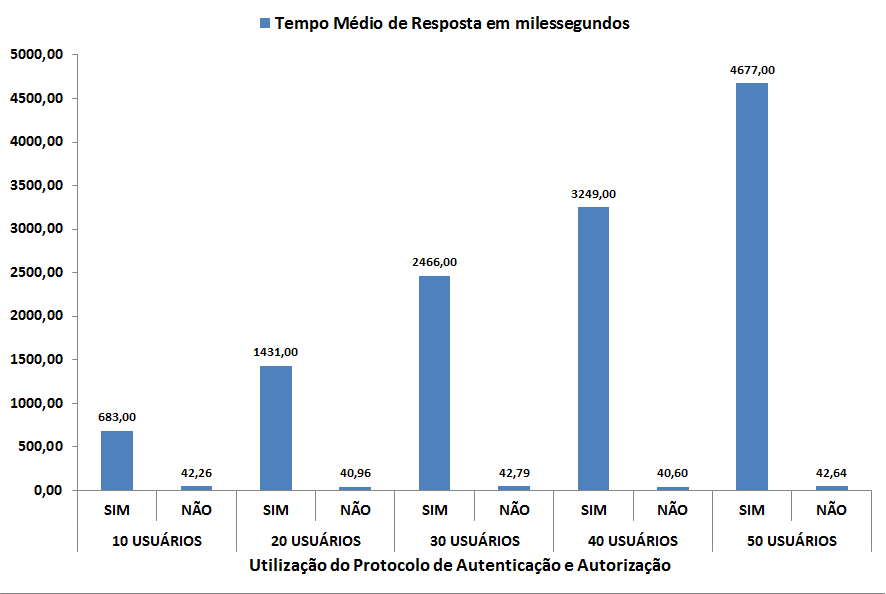
\includegraphics[width=1.0\textwidth]{grafico_teste_desempenho.png}
    \caption{Fluxo do protocolo de autenticação/autorização proposto, 1º cenário.}
    \label{fig:grafico_teste_desempenho}
\end{figure}


\section{Estudo de caso 2}\label{sec:caso2}

Os ambientes de teste utilizados foram o laboratório de informática da Universidade de Brasília e o da Divisão de Tecnologia da Policia Civil do Distrito Federal, uma vez que se busca resultados mais próximos da realidade hoje vivenciado pela PCDF.

Para a realização dos testes foram utilizadas configurações distintas de computadores, conforme apresentado na tabela~\ref{tb:estudo_caso2}.

Os web services adotados serão os mesmos definidos no estudo de caso 1, web service RESTfull de ocorrências criminais, que retornam informações gerais do sistema de ocorrências policiais.

\subsection{\emph{Configuração do ambiente de teste}}

Ambiente de teste foi o da Divisão de Tecnologia da Policia Civil do Distrito Federal, uma vez que se buscam resultados mais próximos da realidade hoje vivenciados pela PCDF.

Para a sua realização dos testes foram utilizados configurações distintas de computadores, conforme tabela abaixo. Essa configuração é idêntica a utilizada no estudo de caso 1.

%\begin{table}[!htpb]
%
%  \begin{tabular}{cp{13cm}}
\begin{table}[h]
    \begin{tabular}{|l|c|p{6cm}|}
    \hline
    \textbf{\emph{Máquina }}                   & \textbf{\emph{Quantidade}} & \textbf{\emph{Configuração}}                                                                               \\ \hline
    Servidor de Autenticação e Autorização  & 1          & Desktop DELL Intel Core I5-2450 2,5 GHz, 4 Gb RAM, 500 HD \\ \hline
    Servidor de Fachada REST  & 1          & Desktop DELL Intel Core I5-2450 2,5 GHz, 4 Gb RAM, 500 HD\\ \hline
    Cliente REST                   & 50        & Desktop DELL Intel Core I5-2450 2,5 GHz, 4 Gb RAM, 500 HD                                    \\ \hline
    \end{tabular}
    \caption {Ambiente de configuração estudo de caso 1}\label{tb:estudo_caso2}
\end{table}

Os servidores de Autenticação e Autorização, Fachada REST e Cliente REST, foram desenvolvidos utilizando a linguagem de programação funcional \emph{Haskell} acessando um banco de dados não relacional, \emph{Apache CouchDB}, conforme apresentado na seção~\ref{sec:implementacao}. O sistema operacional utilizado nessas máquinas foi o Linux Ubuntu 12.04 LTS-64 bits..

\subsection{\emph{Planejamento do experimento}}

O planejamento adotado neste estudo de caso procurou adaptar a realidade vivenciada na PCDF no oferecimento de um serviço. Desta forma, observou-se um cenário extremo de utilização, onde o número médio de requisições aos serviços RESTfull ofertados pela PCDF em 1 hora era de aproximadamente 1200 requisições, ou seja, uma média de duas requisições a cada segundo.

Sendo assim, objetiva-se verificar se o protocolo consegue atender um a caso extremo, que se assemelhe ao vivenciada pela PCDF. Logo, para simular esta situação, realizou-se um teste automatizado, utilizando a ferramenta Apache JMeter, que é um software open source, desenvolvido em Java.

Para realizar o experimento, a abordagem utilizada foi a da utilização de dois fatores: uso do protocolo de autenticação e autorização proposto (SIM/NÃO) e o número de usuários (50) com dois níveis e um nível respectivamente.  Para realizar o experimento foram realizadas 100 requisições para cada usuário, com um intervalo de 2 (dois) segundos de iniciação para cada usuário. As variáveis de resposta adotadas foram o tempo médio de resposta das requisições e a vazão média de requisições por segundo.

\subsection{Análise dos resultados}

A análise dos resultados obtidos com a execução do experimento ocorreu com a observação do tempo médio de resposta e com a verificação da vazão, número de requisições atendidas por segundo, que foi coletado ao final da execução do teste aplicado a um grupo de 50 usuários simultâneos. Dessa forma, foram coletadas 5000(cinco mil) amostras que utilizaram o protocolo de autenticação e autorização proposto em um período de 11 minutos. Os resultados estatísticos são apresentados na tabela~\ref{tb:estatistica_com_cripto_50}.

Em um cenário extremo, observou-se que a PCDF pode ter que responder a uma média de 1200 requisições de um serviço que fornece informações sobre ocorrências policiais em um período de 1 (uma) hora, ou seja, duas requisições a cada um segundo. Neste caso, os resultados obtidos com o experimento realizado com os 50 usuários simultâneos, demonstrou que o tempo médio de resposta foi de 4677 milessegundos ou aproximadamente 4,677 segundos e que a vazão média, que é o número de requisições atendidas por segundo, foi de 8,62 requisições por segundo. Ao se realizar a comparação deste cenário com o cenário extremo vivenciado pela PCDF, verificou-se que a arquitetura, do ponto de vista de vazão, atende perfeitamente o pior caso relatado, que é de 2 duas requisições por segundo. O que garante a qualidade do serviço ofertado pelo protocolo de autenticação e autorização proposto.

\begin{table}[h]
\centering
\begin{tabular}{|l|l|}
\hline
\textbf{Informação} & \textbf{Valor} \\ \hline
Nº de Requisições   &  5000              \\ \hline
Média               &  4677             \\ \hline
Mínimo              &  118          \\ \hline
Máximo              &  21665        \\ \hline
Desvio Padrão       &  3170,49      \\ \hline
\% Erro             &  0,0          \\ \hline
Vazão/seg           &  8,62     \\ \hline
Kbps                &  11,8         \\ \hline
Média de Bytes      &  1401,05      \\ \hline
\end{tabular}
\caption {Estatística básica com a utilização do protocolo de autenticação e autorização para 50 usuários.}\label{tb:estatistica_com_cripto_50}
\end{table}

\section{Síntese do capítulo}
Neste capítulo foram realizados dois estudos de caso, onde foram detalhados os cenários que seriam analisados, os ambientes e planejamento de testes e as referidas análises dos resultados obtidos.

Os estudos de casos realizados evidenciaram que o impacto no desempenho é significativo quando comparado com a não utilização da proposta. Porém os tempos médios obtidos estão dentro de um tempo médio esperado, que é abaixo de 5 segundos. Observou-se ainda, que em um cenário extremo de utilização, onde a PCDF tenha que atender a uma média de 2 duas requisições por segundo, e um período de 1 uma hora, ou seja 1200 requisições, a arquitetura proposta atende perfeitamente, pois consegue atender a 8,62 requisições por segundo em um cenário extremo onde foram realizados 5000 requisições em aproximadamente em 10 minutos.

  %%---------- Quinto Capítulo ----------
\chapter{Análise de Segurança e Desempenho}

Com a definição da arquitetura de referência REST e do protocolo de autenticação e autorização (Capítulo~\ref{cap:Protocolo}), tornou-se necessária a realização de uma análise de segurança e de experimentos que possibilitam a mensuração do impacto da sua utilização no tratamento das requisições realizadas à PCDF.

Este capítulo inicialmente apresenta uma análise dos mecanismos de segurança propostos no protocolo. Essa primeira
análise segue um procedimento informal, mas está de acordo com trabalhos descritos na literatura~\cite{} {\color{red}citar
disserta\c c\~{o}es, teses e artigos que fazem uma an\'{a}lise similar.}. Em seguida, este capítulo apresenta uma avaliação empírica que busca analisar o desempenho do protocolo de Autenticação e Autorização Proposto.

\section{Análise de Segurança}

Nesta seção serão discutidas as propriedades de segurança do protocolo de autenticação e autorização proposto. São abordadas as propriedades e alguns ataques que podem ser realizados. Essa seção segue a estrutura e se fundamenta (parcialmente) no discurso utilizado na análise do protocolo Traust~\cite{traust08}.

\subsection{Segurança da sessão}

O protocolo de Autenticação e Autorização proposto utiliza para segurança de sessão e camada de transporte, o protocolo TLS/SSL. A utilização desse protocolo tem por objetivo evitar o ataque \emph{man-in-the-middle}. Para isso, é exigido, tanto para o órgão conveniado quanto para a própria PCDF, a utilização de certificados digitais padrão X.509, emitidos e garantidos por uma CA que esteja subordinada à hierarquia da ICP-Brasil.

Com isso, ambas as partes envolvidas no processo de comunicação podem estabelecer um processo de confiança mútua no nível de transporte. Todo o tráfego que flui sobre uma sessão bilateral certificada tem uma fonte confiável. Isso permite que implementações de serviços possam autorizar ou desautorizar interações com base na fonte bem conhecida de uma solicitação HTTP.

Além da segurança oferecida pela utilização da segurança na camada de transporte, com utilização do TLS/SSL, o protocolo utiliza mecanismos de segurança tais como criptografia assimétrica e assinatura digital. Isso Permite que outras partes mal intencionadas não consigam ter acesso ao conteúdo das mensagens trocadas pelo protocolo no processo de comunicação.

Diferentemente do sistema Traust~\cite{traust08}, o protocolo de Autenticação e Autorização proposto, será executado apenas em ambientes que tanto o cliente quanto o servidor possuem chaves públicas certificadas. Procura-se, dessa forma, atenuar problemas relacionados ao protocolo TLS, que quando executado em ambientes em que as partes
n\~{a}o possuem chaves públicas certificadas, relacionados a ataques \emph{man-in-the-middle} durante o estabelecimento da sessão~\cite{traust08}.

\subsection{Responsabilização dos usuários conveniados}

Uma das ameaças verificadas diz respeito a possibilidade do uso indevido, por parte dos órgãos conveniados, das informações disponibilizadas nos serviços ofertados pela PCDF. Isso decorre porque as informações disponibilizadas s\~{a}o sensíveis e possuírem caráter sigiloso. Dessa forma, para evitar esse problema é exigido dos órgãos conveniados que assinem um contrato para o consumo do serviço. No momento da assinatura do contrato as institui\c c\~{o}es recebem uma tabela contendo várias credenciais que servem como identidade e que deverão ser utilizadas no processo de autenticação, conforme descrito no seção~\ref{sec:reqprotocolo}. Isso possibilita que ocorra uma autenticação mútua entre a PCDF e os consumidores dos serviços. Além disso, com a utilização do protocolo de autenticação e autorização proposto, são empregados mecanismos de criptografia e assinaturas digitais que são geradas a partir de certificados digitais padrão X.509 vinculados aos órgãos e garantidos por AC. Dessa forma, busca-se evitar o não-repúdio por parte das instituições conveniadas,atribuindo-lhes responsabilidades em caso do mau uso dos serviço ofertados pela PCDF. Logo, uma vez detectado algum tipo de vazamento de dados proveniente dos serviços ofertados o órgão poderá ser identificado e após uma apuração minuciosa, responsabilizado pelos danos causados à PCDF.

\subsection{Ataques de repetição}

Esta ameaça, conforme descrita na Seção~\ref{sec:vulnerabilidadessoa}, se empregada contra o protocolo de autenticação e autorização proposto, tem baixa probabilidade de sucesso. Isso porque utilizamos \emph{timestamps} na maior parte das mensagens trocadas pelo protocolo. Além disso, são gerados números únicos, que identificam os desafios de autenticação gerados e que podem ser utilizados como \emph{nonces}, valores gerados de forma aleat\'{o}ria e que podem ser empregados contra esse tipo de ataque.

\subsection{Ataques de negação de serviço}

Esta ameaça é muito difícil de ser evitada, uma vez que  pode ser fruto de ataques via rede, do consumo excessivo de recursos da máquina  ou, ainda, ser resultante da exploração de qualquer tipo de vulnerabilidade que implique na indisponibilidade do serviço ou de um recurso. O protocolo de autenticação e autorização proposto é baseado no esquema de desafio-resposta. Os desafios são gerados de forma aleatória a partir das credenciais que identificam unicamente os consumidores dos serviços, o que possibilita uma autenticação mútua. Além disso, também são empregados outros mecanismos de segurança como utilização da segurança na camada de transporte e mecanismos de criptografia e assinaturas digitais. Isso minimiza a ameaça de ataques de negação de serviço. Assim como o protocolo Traust~\cite{traust08}, o servidor de autenticação e autorização proposto pode ser replicado para outros servidores, o que possibilita um balanceamento de carga e minimiza a criação de gargalos. Isso permite que o servidor de autenticação seja escalável e esteja disponível em situações críticas, como no caso dos ataques de negação de serviço.


\subsection{Roubo de credenciais de autenticação e autorização}\label{subsec:RouboCred}

O protocolo de autenticação a autorização proposto, após executado corretamente, emite um token de segurança que será utilizado para a obtenção do serviço desejado, conforme apresentado na seção~\ref{sec:ArqProtocolo}. Cabe ressaltar que se um atacante conseguir burlar os mecanismos de segurança utilizados pelo protocolo e conseguir acesso a essa credencial de autenticação e autorização, o atacante terá acesso apenas um serviço, pois o protocolo emite credenciais para um único serviço por vez e com tempo de expiração determinado no momento de sua geração. Essa é uma situação muito difícil de ser verificada, porém caso o extravio de credenciais ocorra, buscamos minimizar o problema com o
isolamento de uma credencial por servi\c co requisitado, diminuindo o impacto que pode ocorrer.

Outro problema que pode ocorrer é o roubo de credenciais de autenticação, que são as credenciais que o órgão conveniado recebe no momento da assinatura do contrato de oferecimento do serviço. Essa credenciais são utilizadas para responder aos desafios que serão realizadas pelo protocolo de autenticação proposto. Caso o extravio o ocorra e seja identificado, a PCDF pode, de forma flex\'{i}vel e transparente, desativar as credenciais que julga terem sido comprometidas sem que o usuário seja prejudicado.
Em um caso mais extremo, outras credenciais podem ser geradas e redistribuídas \`{a}s institui\c c\~{o}es conveniadas.

Porém, cabe ressaltar que, caso ocorra o extravio de credenciais, o órgão que teve o problema será investigado e poderá ser responsabilizado--- caso seja detectada uma m\'{a}
gestão na guarda das credenciais, conforme descrito na subseção~\ref{subsec:RouboCred}


\subsection{Ponto único de ataque}

Uma das possibilidades verificadas é que, ocorrendo um ataque, o alvo possa não ser protocolo de autenticação e autorização proposto e sim o próprio \servidorAA.
Neste caso, se o atacante for bem sucedido o servidor poder ficar vulnerável. Esse servidor é responsável pela geração dos desafios de autenticação e pela geração das credenciais de autenticação e autorização. Porém, apesar de realizar estas atividades ele armazena e consulta os dados gerados no processo de autenticação e autorização em outra máquina, que é em um servidor de banco de dados. Em outras palavras, o \servidorAA está em uma máquina diferente do servidor de banco de dados, o que minimiza os problemas relacionados a esse tipo de ataque, pois o servidor pode ser replicado para outra máquina e o que estiver com problemas pode ser facilmente substituído.

\subsection{S\'{i}ntese da an\'{a}lise de seguran\c ca}

\begin{itemize}
\item descrever os pontos positivos
\item descrever os pontos que requerem mais aten\c c\~{a}o
\end{itemize}

\section{Testes de desempenho}

Testes de desempenho são definidos como investiga\c c\~{o}es técnicas realizadas 
para determinar a capacidade de resposta, a confiabilidade ou escalabilidade de um sistema, 
sob uma determinada carga de trabalho~\cite{Meier2007}.
A análise de desempenho possibilita identificar problemas que geralmente são encontrados em sistemas computacionais. 
Esses problemas podem ser agrupados em termos de comparação e configuração de sistemas, identificação de gargalos, 
caracterização de cargas de trabalho e a previsão de desempenho~\cite{jain1991art}. Dessa forma, foram conduzidos 
experimentos com o objetivo de analisar o desempenho do protocolo de autenticação e autorização proposto. O restante 
dessa se\c c\~{a}o descreve os procedimentos e os resultados obtidos com a an\'{a}lise de desempenho. 
 
\subsection{Objetivos, Questões e Métricas}\label{sec:gqm}

A avaliação de desempenho do protocolo de autenticação e autorização proposto foi organizada com o uso da abordagem 
GQM (\emph{Goals, Questions, and Metrics})~\cite{gqm}. O resultado da aplicação da GQM é a especificação de um sistema de 
medição visando um conjunto particular de problemas e um conjunto de regras para a interpretação dos dados de medição~\cite{gqm}.  
O modelo de avaliação resultante tem três níveis: nível conceitual, onde  são definidos os objetivos da medição; nível operacional, que é aquele 
onde são verificadas as questões  que caracterizam o objeto da medição; e o nível quantitativo, que é o nível onde são definidas as métricas que 
identificam a medidas necessárias para responder as questões levantadas~\cite{gqm}. 

\subsubsection{Objetivos }\label{sec:gqmobjetivos}

A realização de testes de desempenho objetivam determinanr  se o desempenho de um algoritmo, protocolo ou sistema está de acordo com os requisitos. 
Outro objetivo dos testes de desempenho é o de validar a capacidade de resposta, a vazão, a confiabilidade e a escalabilidade de um sistema sob 
uma determinada carga~\cite{Meier2007}. Em rela\c c\~{a}o ao trabalho desenvolvido nessa disserta\c c\~{a}o, 
a avaliação de desempenho do protocolo de autenticação e autorização proposto tem como objetivo:

\begin{itemize}
\item Verificar o impacto do protocolo de autenticação e autorização proposto;
\item Identificar a viabilidade do uso do protocolo em cen\'{a}rios de carga esperados para a PCDF.
\end{itemize}


\subsubsection{Questões}\label{sec:gqmquestoes}

Seguindo o que é preconizado na metodologia GQM, os objetivos são definidos em um nível abstrato, de forma que devem ser formuladas questões, em um nível operacional, que têm por finalidade responder se os objetivos definidos serão atendidos. Logo, com base nos objetivos formulados para a análise de desempenho do protocolo de autenticação e autorização 
proposto, as seguintes questões foram investigadas:

\parbox{0.8\textwidth}{
\begin{enumerate}[(Q1)]
\item \emph{Qual o impacto observado no tempo de resposta às requisições com o uso do protocolo?}
\item \emph{Um protótipo funcional, sem foco em otimização, consegue suportar a demanda prevista?}
\end{enumerate}}

\subsubsection{Métricas}

O desempenho é descrito quantitativamente por meio de métricas. Uma métrica pode ser definida como um conjunto de dados que é definido para responder uma questão de maneira quantitativa. Dessa forma, foram utilizadas as seguintes métricas na avaliação do desempenho do protocolo de autenticação e autorização proposto. 

\begin{itemize}
\item quantidade de usuários: vari\'{a}vel de controle que representa a quantidade de usuários utilizados na avaliação de desempenho.

\item utilização do protocolo: vari\'{a}vel de controle que indica a utiliza\c c\~{a}o ou n\~{a}o do protocolo proposto na disserta\c c\~{a}o. Ela é definida em dois níveis, SIM ou  NÃO.

\item tempo médio de resposta: vari\'{a}vel de resposta que consiste no tempo entre a solicitação de um serviço por um usuário até o momento em que ele recebe uma resposta 
completa~\cite{ Molyneaux2009}. Para a análise de desempenho do protocolo proposto o tempo médio será dado em milissegundos.

\item Vazão (\emph{throughput}): vari\'{a}vel de resposta que corresponde ao número de operações que podem ser tratadas pelo protocolo em um 
determinado período de tempo~\cite{ Molyneaux2009}.

\end{itemize}

Dessa forma, após definir as métricas utilizadas na avaliação de desempenho, foi criado um plano de medição que descreve 
como as vari\'{a}veis de resposta serão mensuradas e quais procedimentos ser\~{a}o realizados 
durante o período de execução dos experimentos.

Logo, o primeiro passo foi a criação de um serviço REST, que retorna informações sobre ocorrências policiais, tais como: 
quais tipos de ocorrências criminais estão registradas, dados gerais da vítima, autor, dentre outras informações. 
Esse serviço é consumido  no momento da execução dos testes de desempenho da solução proposta. 
Foram realizados 10 cen\'{a}rios de testes, conforme representado na Tabela~\ref{tb:tb_testes}.

\begin{table}[h]
\begin{center}
\begin{tabular}{|c|c|c|}
\hline
N. de usuários & Sem utilização do protocolo & Com utilização do Protocolo \\ \hline
10             & Teste 1                     & Teste 2                     \\ \hline
20             & Teste 3                     & Teste 4                    \\ \hline
30             & Teste 5                     & Teste 6                    \\ \hline
40             & Teste 7                     & Teste 8                    \\ \hline
50             & Teste 9                     & Teste 10                    \\ \hline
\end{tabular}
\caption {Cen\'{a}rios de testes realizados}\label{tb:tb_testes}
\end{center}
\end{table}

Para a execução dos testes, que utilizam as métricas definidas, foram estabelecidas as seguintes regras: Cada teste deve realizar várias requisições ao serviço REST 
criado e o número de requisições é obtido pela fórmula $numeroUsuarios \times 100$. A frequência de lançamento das threads, 
que representam os usuários virtuais, é definido pela fórmula $numeroUsuarios \times 2s$. Exemplificando, 
de acordo com a Tabela~\ref{tb:tb_testes}, ao selecionar o Teste 1, serão executadas 10 threads a cada 20 segundos. 
Importa salientar que cada thread corresponde a um usuário, é iniciada 2 segundos após a thread anterior e executa 100 requisições---
o que totaliza 1000 requisições ao serviço no cen\'{a}rio Teste 1. Esse procedimento foi adotado para os demais cen\'{a}rios de testes. 
Por fim, as variáveis de resposta adotadas para a análise de desempenho, conforme discutido, 
foram o tempo médio de resposta das requisições e a vazão média de requisições por segundo.

\subsection{Configuração do ambiente de teste}

O ambiente de teste envolveu estações de trabalho tanto do Laboratório de Engenharia de Software da Universidade de Brasília quanto na 
Divisão de Tecnologia da Policia Civil do Distrito Federal. Para a realização dos testes foram 
utilizadas configurações distintas de computadores, conforme apresentado na tabela~\ref{tb:estudo_caso1}.

\begin{table}[h]
\begin{center}
    \begin{tabular}{|p{6cm}|c|p{6cm}|}
    \hline
    Esta\c c\~{a}o                  & Quantidade & Configura\c c\~{a}o \\ \hline
    Servidor de Autenticação e Autorização     & 1          & Desktop DELL Intel Core I5-2450 2,5 GHz, 4 Gb RAM, 500 HD \\ \hline
    Servidor de Fachada REST                   & 1          & Desktop DELL Intel Core I5-2450 2,5 GHz, 4 Gb RAM, 500 HD \\ \hline
    Cliente REST                               & 1          & Desktop DELL Intel Core I5-2450 2,5 GHz, 4 Gb RAM, 500 HD \\ \hline
    Servidor do Serviço web REST PCDF       & 1          & Intel Xeon E7 4870 2,4 GHz, 8 Gb RAM, 120 HD \\ \hline
    \end{tabular}
    \caption {Ambiente utilizado na análise de desempenho}\label{tb:estudo_caso1}
\end{center}
\end{table}

Os servidores de Autenticação e Autorização, Fachada REST e Cliente REST, foram prototipados utilizando a linguagem de programação funcional \emph{Haskell}. Estes 
servidores acessam uma base de dados não relacional \emph{CouchDB}, conforme apresentado na seção~\ref{sec:implementacao}. 
O sistema operacional utilizado nessas máquinas foi o Linux Ubuntu 12.04 LTS-64 bits. No caso do serviço REST desenvolvido pela PCDF, 
para atender a demanda da análise de desempenho, foi desenvolvido utilizando a linguagem C\# acessando um banco de dados \emph{SQL Server 2008 r2} 
que mant\'{e}m os registros das ocorr\^{e}ncias policiais. O serviço foi publicado em um servidor que utiliza o sistema operacional 
\emph{Windows Server 2008 r2, Enterprise Edition x64}, utilizando o ISS 7.0 como servidor Web. 
A Figura~\ref{fig:ambiente_teste} descreve os ambientes de configuração utilizados na análise de desempenho do {\color{red}(tem que padronizar. em 
alguns pontos est\'{a} mai\'{u}sculo, em outros min\'{u}sculo)Protocolo de Autenticação e Autorização proposto}.


\begin{figure}[!htb]
\centering
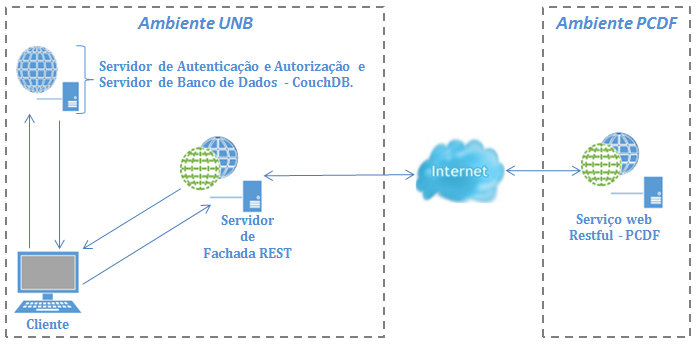
\includegraphics[width=0.8\textwidth]{ambiente_teste_desempenho.png}
\caption{Ambiente de teste de desempenho do Protocolo de Autenticação e Autorização.}
\label{fig:ambiente_teste}
\end{figure}

\subsection{Análise dos resultados}

Os testes objetivam (a) verificar o impacto no tempo de resposta às requisições com o uso do protocolo e (b) avaliar se um protocolo funcional, sem foco em otimização, 
suportaria a demanda de requisi\c c\~{o}es prevista para a PCDF. Para atender aos objetivos supracitados, foram realizados testes considerando 
requisi\c c\~{o}es diretas, sem o uso do protocolo de autentica\c c\~{a}o e autoriza\c c\~{a}o; e requisi\c c\~{o}es seguras e que seguem as trocas 
de mensagens definidas no protocolo. Conforme discutido nas se\c c\~{o}es anteriores, as an\'{a}lises resultaram em um universo de amostras
com 1000, 2000, 3000, 4000 e 5000 requisi\c c\~{o}es, correspondendo respectivamente a grupos de 10, 20, 30, 40 e 50 usuários. 
Os dados coletados foram analisados, e resultados estatísticos são apresentados nas  tabelas~\ref{tb:estatistica_com_cripto} e ~\ref{tb:estatistica_sem_cripto}. 

Dessa forma, com o objetivo de responder a primeira questão relacionada ao teste de performance 
(\emph{Qual o impacto observado no tempo de resposta às requisições com o uso do protocolo?}), 
consideramos que os resultados obtidos evidenciam um impacto significativo com a utilização do protocolo de autenticação e autorização proposto. 
Pode-se observar que, com a utilização do protocolo para 10 usuários simultâneos, o tempo médio de resposta é de 683,84 milissegundos. 
Por outro lado, quando comparado ao acesso ao serviço sem a utilização do protocolo, o tempo médio de resposta às requisições é de 42,26 milissegundos. 
Estas comparações estendem-se aos demais cen\'{a}rios de testes, para 20, 30, 40 e 50 usuários. Em todos casos o impacto é significativo quando comparado 
aos resultados obtidos sem a utilização do protocolo de autenticação e autorização. Porém, essa variação era de certa forma esperada, pois o protocolo proposto 
incorpora mecanismos de segurança que requerem algoritmos de criptografia e assinatura digital e segurança na camada de transporte com a utilização do SSL/TLS. 
Além disso, a implementação do protocolo será ainda alvo de otimizações.

De outra forma, ao analisar o tempo médio dos experimentos que utilizaram o protocolo, nota-se que este tempo é aceitável, pois com 10 usuários ele fica abaixo de 1 segundo, com 20 o tempo médio é 1,5 segundos, com 30 usuários esse tempo sobe para aproximadamente 2,5 segundos, aumentado de forma aceitável até 50 usuários em que o tempo médio verificado foi de aproximadamente 4,5 segundos, conforme apresentado nas tabelas ~\ref{tb:estatistica_com_cripto} e ~\ref{tb:estatistica_sem_cripto} e no gráfico ~\ref{fig:grafico_teste_desempenho}. De forma que esses resultados estão dentro do esperado para utilização. Atualmente o número de convênios na PCDF não supera 10 usuários, estima-se que com a utilização do protocolo esse número suba para no máximo 30 órgãos conveniados. Logo, com a análise dos resultados percebe-se que, apesar do impacto da utilização do protocolo de autenticação e autorização, o tempo m\'{e}dio de resposta não configura como um limitador para sua utilização. {\color{red}Relaciona com os estudos que avaliam o impacto no tempo de resposta com a 
ado\c c\~{a}o de WS-Security, WS-*.}


\begin{table}[h]
\begin{center}
\begin{tabular}{|c|c|c|c|c|c|}
\hline
%\multicolumn{6}{|p{15cm}|}{\textbf{\begin{tabular}[c]{@{}c@{}}   TEMPO DE RESPOSTA COM A UTILIZAÇÃO \\      DO PROTOCOLO DE AUTENTICAÇÃO E AUTORIZAÇÃO \end{tabular}}} \\ \hline
%\multicolumn{1}{|l|}{Qtd Usuários}    & Tempo Médio   & Erro Padrão & Mediana  & Desv Padrão  & Qtd Req. \\ \hline
Qtd Usuários    & Tempo Médio   & Erro Padrão & Mediana  & Desv Padrão  & Qtd Req. \\ \hline
10                                    & 683,84        & 12,53       & 622,5    & 396,36       &  1000       \\ \hline
20                                    & 1.431,14      & 21,63       & 1.274,5  & 967,30       &  2000       \\ \hline
30                                    & 2.466,28      & 35,86       & 2.067    & 1964,30      &  3000       \\ \hline
40                                    & 3.249,76      & 35,83       & 3.084,5  & 2266,50      &  4000       \\ \hline
50                                    & 4.677,64      & 44,84       & 4.375,5  & 3170,80      &  5000       \\ \hline
\end{tabular}\caption {An\'{a}lise de desempenho considerando o protocolo de autenticação e autorização.}\label{tb:estatistica_com_cripto}
\end{center}
\end{table}

\begin{table}[h]
\begin{center}
\begin{tabular}{|c|c|c|c|c|c|}
\hline
%\multicolumn{6}{|p{15cm}|}{\textbf{\begin{tabular}[c]{@{}c@{}}TEMPO DE RESPOSTA SEM UTILIZAÇÃO \\ DO PROTOCOLO DE AUTENTICAÇÃO E AUTORIZAÇÃO\end{tabular}}} \\ \hline
%\multicolumn{1}{|l|}{Qtd Usuários}    & Tempo Médio    & Erro Padrão & Mediana  & Desv Padrão & Qtd Req. \\ \hline
Qtd Usuários    & Tempo Médio    & Erro Padrão & Mediana  & Desv Padrão & Qtd Req. \\ \hline
10                                    & 42,26          & 1,12        & 43       & 35,51       &  1000       \\ \hline
20                                    & 40,96          & 0,65        & 39       & 29,35       &  2000       \\ \hline
30                                    & 42,79          & 1,20        & 37       & 65,97       &  3000       \\ \hline
40                                    & 40,60          & 0,40        & 43       & 25,69       &  4000       \\ \hline
50                                    & 42,64          & 0,48        & 44       & 34,39       &  5000       \\ \hline
\end{tabular}\caption {An\'{a}lise de desempenho sem considerar o protocolo de autenticação e autorização.}\label{tb:estatistica_sem_cripto}
\end{center}
\end{table}

Al\'{e}m disso, a quantidade de usuários simultâneos tem impacto no desempenho da aplicação SOA 
que utiliza o protocolo de autenticação e autorização proposto. Verifica-se que o tempo médio de resposta 
sobe de acordo com a quantidade de usuários. No caso da não utilização do protocolo, observa-se que o tempo médio 
de resposta é constante e que a variação não \'{e} tão significante com o aumento do número de usuários simultâneos,
 conforme observado na figura~\ref{fig:grafico_teste_desempenho}.

\begin{figure}[!htb]
    \centering
    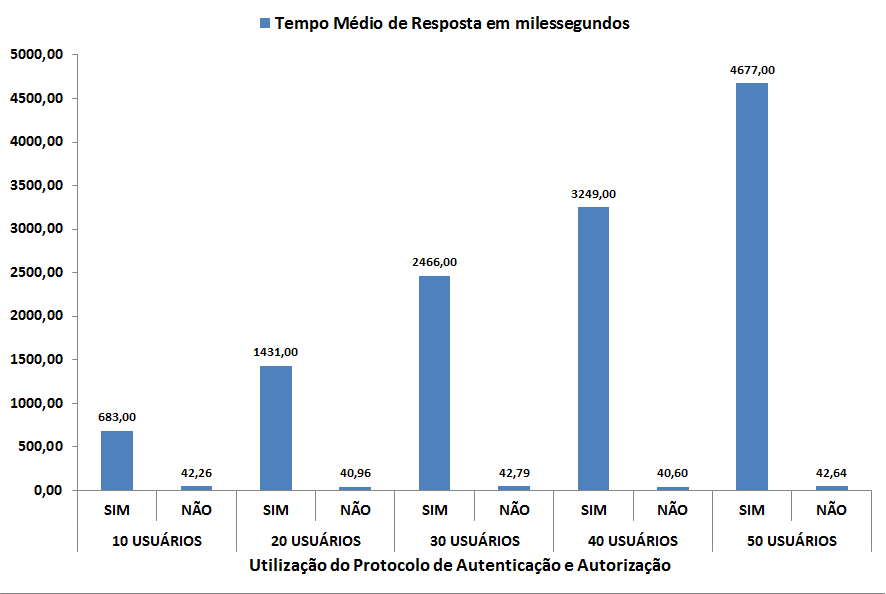
\includegraphics[width=1.0\textwidth]{grafico_teste_desempenho.png}
    \caption{Fluxo do protocolo de autenticação/autorização proposto, 1º cenário.}
    \label{fig:grafico_teste_desempenho}
\end{figure}

Para responder a segunda questão relacionada \`{a} an\'{a}lise de desemepenho (\emph{Um protótipo funcional, sem foco em otimização, consegue suportar a demanda prevista?}), 
novamente foram realizadas análises dos dados coletados nos testes realizados. A análise dos resultados obtidos com a execução do experimento ocorreu com a observação do tempo médio de resposta e com a verificação da vazão--- ou seja, o número de requisições atendidas por segundo, que foi coletado ao final da execução do Teste 10, aplicado a um grupo de 50 usuários, conforme apresentado na Tabela~\ref{tb:tb_testes}. Dessa forma, foram coletadas 5000 amostras que utilizaram o 
protocolo de autenticação e autorização proposto em um período de 11 minutos {\color{red}por que 11 minutos?}. Os resultados estatísticos são apresentados na tabela~\ref{tb:estatistica_com_cripto_50}.

Observa-se que a PCDF, em um cenário extremo, pode ter que responder a uma média de 1200 requisições de um serviço que fornece informações sobre ocorrências policiais em um período de uma hora, ou seja, duas requisições por segundo. Neste caso, os resultados obtidos com o experimento realizado com os 50 usuários, demonstrou que o tempo médio de resposta foi de 4677 milissegundos (ou aproximadamente 4,677 segundos) e que a vazão média, que é o número de requisições atendidas por segundo, foi de 8,62 requisições por segundo. Ao se realizar a comparação deste cenário com o cenário extremo vivenciado pela PCDF, verificou-se que a arquitetura, do ponto de vista de vazão, atende ao cen\'{a}rio mais cr\'{i}tico, 
que é de 2 duas requisições por segundo. O que garante a qualidade do serviço ofertado pelo protocolo de autenticação e autorização proposto.

{\color{red}essa tabela est\'{a} muito ruim. sugiro remover} 

\begin{table}[h]
\centering
\begin{tabular}{|l|l|}
\hline
\textbf{Informação} & \textbf{Valor} \\ \hline
Nº de Requisições   &  5000              \\ \hline
Média               &  4677             \\ \hline
Mínimo              &  118          \\ \hline
Máximo              &  21665        \\ \hline
Desvio Padrão       &  3170,49      \\ \hline
\% Erro             &  0,0          \\ \hline
Vazão/seg           &  8,62     \\ \hline
Kbps                &  11,8         \\ \hline
Média de Bytes      &  1401,05      \\ \hline
\end{tabular}
\caption {Estatística básica com a utilização do protocolo de autenticação e autorização para 50 usuários.}\label{tb:estatistica_com_cripto_50}
\end{table}

\section{Síntese do capítulo}

{\color{red} revisa essa s\'{i}ntese. est\'{a} furada. fala apenas do teste de desempenho} 

Neste cap\'{i}tulo foi realizada uma análise de desempenho, onde foram definidos objetivos e questões que foram respondidas após a execução e análise dos testes realizados. O estudo evidenciou que o impacto no desempenho é significativo quando comparado com a não utilização da proposta. Porém os tempos médios obtidos estão dentro de um tempo médio esperado, que é abaixo de 5 segundos. Observou-se ainda, que em um cenário extremo de utilização, onde a PCDF tenha que atender a uma média de 2 duas requisições por segundo, e um período de 1 uma hora, ou seja 1200 requisições, a arquitetura proposta atende perfeitamente, pois consegue atender a 8,62 requisições por segundo em um cenário extremo onde foram realizados 5000 requisições em aproximadamente em 10 minutos. 
   \chapter{Conclusão}%

A Polícia Civil do Distrito Federal tem a necessidade de integrar e compartilhar informações sensíveis com órgãos conveniados. Devido à criticidade dessas informações, preocupações relacionadas à segurança foram levantadas e devem ser tratadas sob uma perspectiva arquitetural.

Nesse sentido, este trabalho teve como objetivo propor um Protocolo de Autenticação e Autorização seguro, baseado no modelo desafio-resposta, que possibilitasse a integração segura das informações disponibilizadas por meio de uma arquitetura orientada a serviços. O protocolo foi desenvolvido aderente à arquitetura REST e incorpora mecanismos de segurança tais como: criptografia, assinatura digital e uso de certificados digitais. Dessa forma, ele atende aos requisitos básicos de segurança: autenticidade, integridade, confidencialidade e disponibilidade.

Um ponto importante no desenvolvimento do trabalho foi a utilização da lógica BAN, para analisar formalmente o  protocolo proposto, haja vista que ela é uma lógica pioneira utilizada para analisar protocolos criptográficos. Com a realização do trabalho foi possível ampliar os conhecimentos sobre SOA, mecanismos de segurança, integração utilizando web services e serviços baseados na arquitetura REST. Além disso, também foi possível realizar análises de desempenho e de segurança do protocolo e em ambos os casos o protocolo se mostrou confiável e viável.

A utilização do Protocolo de Autenticação e Autorização proposto, por parte da PCDF, possibilitará que as informações críticas que antes não eram compartilhadas por não haver formas seguras de compartilhamento das informações dentro da Instituição, possam agora ser compartilhadas e efetivamente integradas de forma eficiente e principalmente segura com os órgãos parceiros. A solução proposta neste trabalho vai ao encontro ao que a PCDF almejava. Além disso, a solução proposta pode ser utilizada por qualquer órgão de segurança, que da mesma forma, tenha a necessidade de compartilhar e integrar informações sensíveis.

Quanto a trabalhos futuros, vislumbramos a possibilidade de se implementar otimizações ao Protocolo de Autenticação e Autorização proposto, de forma que ele possa ser melhorado sob o aspecto de desempenho. Outros pontos que também serão realizados, são estudos mais aprofundados sobre possíveis vulnerabilidades tanto do lado do cliente, consumidor do serviço,  quanto do lado da PCDF, provedora dos serviços.


  %%---------- Quinto Capítulo ----------
\chapter{Análise de Segurança e Desempenho}

Com a definição da arquitetura de referência \emph{REST}  e do protocolo de autenticação e autorização (Capítulo~\ref{cap:Protocolo}),
tornou-se necess\'{a}ria a realiza\c c\~{a}o de uma an\'{a}lise de seguran\c ca e de experimentos que possibilitam a mensuração do
impacto da sua utilização no tratamento das requisi\c c\~{o}es realizadas \`{a} PCDF. Neste caso, procedemos com
a investiga\c c\~{a}o das seguintes quest\~{o}es

\parbox{0.8\textwidth}{
\begin{enumerate}[(Q1)]
\item \emph{Qual o impacto observado no tempo de resposta às requisi\c c\~{o}es com o uso do protocolo?}
\item \emph{Um prot\'{o}tipo funcional, sem foco em otimiza\c c\~{a}o, consegue suportar a demanda prevista?}
\end{enumerate}}


Este capítulo inicialmente apresenta uma análise dos mecanismos de segurança propostos no protocolo. Essa primeira
análise segue um procedimento informal, mas está de acordo com trabalhos descritos na literatura~\cite{} {\color{red}citar
disserta\c c\~{o}es, teses e artigos que fazem uma an\'{a}lise similar.}. Em seguida, este capítulo apresenta uma avaliação empírica que busca analisar o desempenho do protocolo de Autenticação e Autorização Proposto.
\section{Análise de Segurança}

Nesta seção serão discutidas as propriedades de segurança do protocolo de autenticação e autorização proposto. São abordadas as propriedades e alguns ataques que podem ser realizados. Essa seção segue a estrutura e se fundamenta (parcialmente) no discurso utilizado na an\'{a}lise do protocolo Traust~\cite{traust08}.

\subsection{Segurança da sessão}

O protocolo de Autenticação e Autorização proposto utiliza para segurança de sessão e camada de transporte, o protocolo
TLS/SSL. A utilização desse protocolo tem por objetivo evitar o ataque \emph{man-in-the-middle}. Para isso, é exigido, tanto para o órgão conveniado quanto para a própria
PCDF, a utiliza\c c\~{a}o de certificados digitais padrão X.509, emitidos e garantidos por uma {\color{red}AC (caso essa sigla n\~{a}o tenha sido usada antes,
definir o significado aqui)} que esteja subordinada à hierarquia da ICP-Brasil.

Com isso, ambas as partes envolvidas no processo de comunicação podem estabelecer um processo de confiança mútua no nível de transporte. Todo o tráfego que flui sobre uma sessão bilateral certificada tem uma fonte confiável. Isso permite que implementações de serviços possam autorizar ou desautorizar interações com base na fonte bem conhecida de uma solicitação HTTP.

Além da segurança oferecida pela utilização da segurança na camada de transporte, com utilização do TLS/SSL, o protocolo utiliza mecanismos de segurança tais como
criptografia assimétrica e assinatura digital. Isso Permite que outras partes mal intencionadas não consigam ter acesso ao conteúdo das mensagens trocadas pelo protocolo
no processo de comunicação.

Diferentemente do sistema Traust~\cite{traust08}, o protocolo de Autenticação e Autorização proposto, será executado apenas em ambientes que tanto o cliente quanto o servidor possuem chaves públicas certificadas. Procura-se, dessa forma, atenuar problemas relacionados ao protocolo TLS, que quando executado em ambientes em que as partes
n\~{a}o possuem chaves públicas certificadas, relacionados a ataques \emph{man-in-the-middle} durante o estabelecimento da sessão~\cite{traust08}.

\subsection{Responsabilização dos usuários conveniados}

Uma das ameaças verificadas diz respeito a possibilidade do uso indevido, por parte dos órgãos conveniados, das informações disponibilizadas nos serviços ofertados pela PCDF. Isso decorre porque as informações disponibilizadas s\~{a}o sensíveis e possuírem caráter sigiloso. Dessa forma, para evitar esse problema é exigido dos órgãos conveniados que assinem um contrato para o consumo do serviço. No momento da assinatura do contrato as institui\c c\~{o}es recebem uma tabela contendo várias credenciais que servem como identidade e que deverão ser utilizadas no processo de autenticação, conforme descrito no seção~\ref{sec:reqprotocolo}. Isso possibilita que ocorra uma autenticação mútua entre a PCDF e os consumidores dos serviços. Além disso, com a utilização do protocolo de autenticação e autorização proposto, são empregados mecanismos de criptografia e assinaturas digitais que são geradas a partir de certificados digitais padrão X.509 vinculados aos órgãos e garantidos por AC. Dessa forma, busca-se evitar o não-repúdio por parte das institui\c c\~{o}es conveniadas,
atribuindo-lhes responsabilidades em caso do mau uso dos serviço ofertados pela PCDF. Logo, uma vez detectado algum tipo de vazamento de dados proveniente dos serviços ofertados o órgão poderá ser identificado e após uma apuração minuciosa, responsabilizado pelos danos causados à PCDF.

\subsection{Ataques de repetição}

Esta ameaça, conforme descrita na Seção~\ref{sec:vulnerabilidadessoa}, se empregada contra o protocolo de autenticação e autorização proposto, tem baixa probabilidade de sucesso.
 Isso porque utilizamos \emph{timestamps} na maior parte das mensagens trocadas pelo protocolo. Além disso, são gerados números únicos, que identificam os desafios de autenticação gerados e que podem ser utilizados como \emph{nonces}--- valores gerados de forma aleat\'{o}ria e que podem ser empregados contra esse tipo de ataque.

\subsection{Ataques de negação de serviço}

Esta ameaça é muito difícil de ser evitada, uma vez que  pode ser fruto de ataques via rede, do consumo excessivo de recursos da máquina  ou, ainda, ser resultante da exploração de qualquer tipo de vulnerabilidade que implique na indisponibilidade do serviço ou de um recurso. O protocolo de autenticação e autorização proposto é baseado no esquema de desafio-resposta. Os desafios são gerados de forma aleatória a partir das credenciais que identificam unicamente os consumidores dos serviços, o que possibilita uma autenticação mútua. Além disso, também são empregados outros mecanismos de segurança como utilização da segurança na camada de transporte e mecanismos de criptografia e assinaturas digitais. Isso minimiza a ameaça de ataques de negação de serviço. Assim como o protocolo Traust~\cite{traust08}, o servidor de autenticação e autorização proposto pode ser replicado para outros servidores, o que possibilita um balanceamento de carga e minimiza a criação de gargalos. Isso permite que o servidor de autenticação seja escalável e esteja disponível em situações críticas, como no caso dos ataques de negação de serviço.


\subsection{Roubo de credenciais de autenticação e autorização}\label{subsec:RouboCred}

O protocolo de autenticação a autorização proposto, após executado corretamente, emite um token de segurança que será utilizado para a obtenção do serviço desejado, conforme
apresentado na seção~\ref{sec:ArqProtocolo}. Cabe ressaltar que se um atacante conseguir burlar os mecanismos de segurança utilizados pelo protocolo e conseguir acesso a essa credencial de autenticação e autorização, o atacante terá acesso apenas um serviço, pois o protocolo emite credenciais para um único serviço por vez e com tempo de expiração determinado no momento de sua geração. Essa é uma situação muito difícil de ser verificada, porém caso o extravio de credenciais ocorra, buscamos minimizar o problema com o
isolamento de uma credencial por servi\c co requisitado, diminuindo o impacto que pode ocorrer.

Outro problema que pode ocorrer é o roubo de credenciais de autenticação, que são as credenciais que o órgão conveniado recebe no momento da assinatura do contrato de oferecimento do serviço. Essa credenciais são utilizadas para responder aos desafios que serão realizadas pelo protocolo de autenticação proposto. Caso o extravio o ocorra e seja identificado, a PCDF pode, de forma flex\'{i}vel e transparente, desativar as credenciais que julga terem sido comprometidas sem que o usuário seja prejudicado.
Em um caso mais extremo, outras credenciais podem ser geradas e redistribuídas \`{a}s institui\c c\~{o}es conveniadas.

Porém, cabe ressaltar que, caso ocorra o extravio de credenciais, o órgão que teve o problema será investigado e poderá ser responsabilizado--- caso seja detectada uma m\'{a}
gestão na guarda das credenciais, conforme descrito na subseção~\ref{subsec:RouboCred}


\subsection{Ponto único de ataque}

Uma das possibilidades verificadas é que, ocorrendo um ataque, o alvo possa não ser protocolo de autenticação e autorização proposto e sim o próprio \servidorAA.
Neste caso, se o atacante for bem sucedido o servidor poder ficar vulnerável. Esse servidor é responsável pela geração dos desafios de autenticação e pela geração das credenciais de autenticação e autorização. Porém, apesar de realizar estas atividades ele armazena e consulta os dados gerados no processo de autenticação e autorização em outra máquina, que é em um servidor de banco de dados. Em outras palavras, o \servidorAA está em uma máquina diferente do servidor de banco de dados, o que minimiza os problemas relacionados a esse tipo de ataque, pois o servidor pode ser replicado para outra máquina e o que estiver com problemas pode ser facilmente substituído.

\subsection{S\'{i}ntese da an\'{a}lise de seguran\c ca}

\begin{itemize}
\item descrever os pontos positivos
\item descrever os pontos que requerem mais aten\c c\~{a}o
\end{itemize}

\section{Testes de desempenho}

Testes de desempenho são definidos como uma investigação técnica realizada para determinar a capacidade de resposta, confiabilidade e / ou escalabilidade de um sistema, sob uma determinada carga de trabalho~\cite{Meier2007}.
A análise de desempenho possibilita identificar problemas que geralmente são encontrados em sistemas computacionais. Esses problemas podem ser agrupados em termos da comparação e configuração de sistemas, identificação de gargalos, caracterização de cargas de trabalho e a previsão de desempenho~\cite{jain1991art}. Sendo assim, a análise de desempenho do protocolo de autenticação e autorização proposto foi dividida em dois estudos de caso que {\color{red}objetivam, respectivamente \ldots}. Esses estudos de caso
são apresentados nas seções~\ref{sec:caso1} e ~\ref{sec:caso2}. {\color{red}temos que conversar sobre o titulo das proximas secoes}

\subsection{Objetivos,Questões e Métricas}\label{sec:caso1}

Nesta seção será apresentada a metodologia empregada para a realização do teste de desempenho bem como os resultados e análise obtidos com sua aplicação.

Para este estudo de caso foi utilizado um serviço web REST que retorna informações sobre as ocorrências policiais, tais como: quais tipos de ocorrências criminais estão registras, dados gerais da vítima, autor, dentre outras informações. Esse serviço web é amplamente utilizado pela PCDF e também pelos seus órgãos parceiros. {\color{red}mas, pelo que eu lembro, esse servi\c co nao era parametrizado. caracterizar melhor para nao criar uma expectativa errada por parte dos revisores} O serviço foi consumido utilizando o protocolo de segurança proposto, buscando-se realizar uma comparação de desempenho com e sem a sua utilização. Como métrica de avaliação verificou-se o tempo médio de resposta, que consiste no tempo entre a solicitação de um serviço por um usuário até o momento em que ele recebe uma resposta completa na sua estação de trabalho~\cite{ Molyneaux2009}.

\subsection{Configuração do ambiente de teste}

O ambiente de teste envolveu est\c c\~{o}es de trabalho tanto do Laboratório de Engenharia de Software da Universidade de Brasília quanto da Divisão de Tecnologia da Policia Civil do Distrito Federal. Para a realização dos testes foram utilizadas configurações distintas de computadores, conforme apresentado na tabela~\ref{tb:estudo_caso1}.
%\begin{table}[!htpb]
%
%  \begin{tabular}{cp{13cm}}
\begin{table}[h]
    \begin{tabular}{|l|c|p{6cm}|}
    \hline
    \textbf{\emph{Máquina }}                   & \textbf{\emph{Quantidade}} & \textbf{\emph{Configuração}}                                                                               \\ \hline
    Servidor de Autenticação e Autorização  & 1          & Desktop DELL Intel Core I5-2450 2,5 GHz, 4 Gb RAM, 500 HD \\ \hline
    Servidor de Fachada REST  & 1          & Desktop DELL Intel Core I5-2450 2,5 GHz, 4 Gb RAM, 500 HD\\ \hline
    Cliente REST                   & {\color{red}50 (errado)}       & Desktop DELL Intel Core I5-2450 2,5 GHz, 4 Gb RAM, 500 HD                                    \\ \hline
    \end{tabular}
    \caption {Ambiente de configuração estudo de caso 1}\label{tb:estudo_caso1}
\end{table}

Os servidores de Autenticação e Autorização, Fachada REST e Cliente REST, foram desenvolvidos utilizando a linguagem de programação funcional \emph{Haskell} acessando um banco de dados não relacional, \emph{Apache CouchDB}, conforme apresentado na seção~\ref{sec:implementacao}. O sistema operacional utilizado nessas máquinas foi o Linux Ubuntu 12.04 LTS-64 bits.


%É importante frisar que essa estrutura foi utilizada em conjunto com os seguintes softwares: sistema operacional Windows Server 2008 R2 Enterprise Edition x64, utilizando o ISS 7.0 como servidor Web, para o Provedor de Serviço de Ocorrências Já o provedor de Banco de dados é o SQL 2008 r2 que utiliza o mesmo sistema operacional. No que tange aos servidores de Autenticação e Autorização, Fachada REST e Cliente REST o sistema operacional utilizado foi o Linux Ubuntu 12.04 LTS-64 bits.

\subsection{Planejamento do experimento}

{\color{red}Necess\'{a}rio reorganizar essa se\c c\~{a}o. Uma alternativa \'{e} apresentar a descri\c c\~{a}o de acordo com as fases de um teste de desempenho. Outra alternativa \'{e} organizar
pelos resultados de cada fase. Est\'{a} muito confuso.}

{\color{red}A an\'{a}lise de desempenho requer um planejamento criterioso, com o intuito de} identificar os cenários de uso, a determinação da variabilidade entre os usuários, a identificação e geração dos dados de teste e a especificação das métricas que serão coletadas. Em síntese, o planejamento possibilita a cria\c c\~{a}o das bases e
perfis para cargas de trabalho~\cite{Meier2007}. Os termos que mais se destacam e que são utilizados durante a etapa do {\color{red} projeto (ou planejamento, tem que padronizar)}
e dos experimentos de um teste de desempenho são: as Variáveis de Resposta, Fatores, Níveis e Interação~\cite{jain1991art}.

As Variáveis de resposta são as medidas de desempenho do sistema e representam o resultado de um experimento. Os Fatores, são termos relacionados com variáveis que influenciam na resposta do sistema. Os Níveis tem relação direta com os valores que um fator pode assumir. Finalmente a Interação, que aponta a dependência entre os fatores que foram avaliados.
Dessa forma, com intuito de verificar qual o impacto de desempenho que o protocolo de autenticação e autorização proposto, apresentado na seção~\ref{sec:implementacao}, tem sobre os serviços oferecidos pela PCDF, optou-se por realizar um teste automatizado, utilizando a ferramenta Apache JMeter. {\color{red}Rog\'{e}rio, reler essa se\c c\~{a}o e melhor\'{a}-la. Precisa
ter um melhor encadeamento com as se\c c\~{o}es anteriores e postoriores. A narrativa est\'{a} destoando do restante do texto. O que a escolha do JMeter tem a ver com as vari\'{a}veis de resposta, fatores, \ldots. Mais ainda, a vari\'{a}vel resposta foi introduzida na se\c c\~{a}o anterior--- antes do planejamento do experimento. Reescrever e me responder indicando os ajustes que foram feitos}.

Sendo assim, a abordagem utilizada foi a da utilização de dois fatores: uso do protocolo de autenticação e autorização proposto ({\color{red} com os n\'{i}veis SIM/NÃO})
e o número de usuários (10, 20,30,40 e 50) com dois e cinco níveis respectivamente {\color{red}reescrever}.
Para realizar o experimento foram realizadas 100 requisições para cada usuário, com um intervalo de 2(dois) segundos para cada grupos de usuários, sendo adotado um índice de 95\% para intervalo de confiança. Já a variável de resposta adotada, foi o tempo médio de resposta das requisições. {\color{red}Justificar essas decis\~{o}es. Essa \'{e} a parte mais fr\'{a}gil do texto
at\'{e} aqui. N\~{a}o podemos apenas elencar os fatores / n\'{i}veis, temos que apresentar as justificativas. }

\subsection{Análise dos resultados}

A análise dos resultados obtidos com a execução do teste de desempenho ocorreu com a observação do tempo de resposta que foi coletado ao final de cada execução dos testes aplicados ao grupos de usuários. Dessa forma, foram coletadas 1000, 2000, 3000, 4000 e 5000 amostras para o grupo de 10, 20, 30, 40 e 50 usuários {\color{red}discutir melhor essa configura\c c\~{a}o, n\~{a}o pode ser econ\^{o}mico nessa parte do texto}; com e sem a utilização do protocolo de autenticação e autorização proposto. Os resultados estatísticos são apresentados nas tabelas~\ref{tb:estatistica_com_cripto} e ~\ref{tb:estatistica_sem_cripto}.

Os resultados obtidos evidenciaram o impacto da utilização do protocolo de autenticação e autorização proposto. Pode-se observar que, com a utilização do protocolo para 10 usuários simultâneos, o tempo médio de resposta é de 683,84 milessegundos. Por outro lado, quando comparado ao acesso ao serviço sem a utilização do protocolo, o tempo m\'{e}dio de
resposta \`{a}s requisi\c c\~{o}es \'{e} de 42,26 milissegundos. Estas comparações estendem-se aos demais experimentos, para 20, 30, 40 e 50 usuários simultâneos. Em todos casos o impacto é significativo quando comparado aos resultados obtidos sem a utilização do protocolo de autenticação e autorização. Porém, essa variação já era esperada, pois o protocolo proposto incorpora mecanismos de segurança que requerem algoritmos de criptografia e assinatura digital e segurança na camada de transporte com a utilização do SSL/TLS. Al\'{e}m disso
 a implementa\c c\~{a}o do protocolo n\~{a}o ainda ser\'{a} alvo de otimiza\c c\~{o}es.

De outra forma, ao analisar o tempo médio dos experimentos que utilizaram o protocolo, nota-se que este tempo é aceitável, pois com 10 usuários ele fica abaixo de 1 segundo, com 20 o tempo médio é 1,5 segundos, com 30 usuários esse tempo sobe para aproximadamente 2,5 segundos, aumentado de forma aceitável até 50 usuários em que o tempo médio verificado foi de aproximadamente 4,5 segundos, conforme apresentado nas tabelas ~\ref{tb:estatistica_com_cripto} e ~\ref{tb:estatistica_sem_cripto} e no gráfico ~\ref{fig:grafico_teste_desempenho}. De forma que esses resultados estão dentro do esperado para utilização. Atualmente o número de convênios na PCDF não supera 10 usuários, estima-se que com a utilização do protocolo esse número suba para no máximo 30 órgãos conveniados. Logo, com a análise dos resultados percebe-se que apesar do impacto da utilização do protocolo de autenticação e autorização, o tempo de resposta médio obtido não configura como um limitador para sua utilização.


\begin{table}[h]
\begin{tabular}{|c|c|c|c|c|c|c|c|c|c|}
\hline
\multicolumn{7}{|c|}{\textbf{\begin{tabular}[c]{@{}c@{}}TEMPO DE RESPOSTA COM A UTILIZAÇÃO \\ DO PROTOCOLO DE AUTENTICAÇÃO E AUTORIZAÇÃO EM MILISSEGUNDOS\end{tabular}}} \\ \hline
\multicolumn{1}{|l|}{Qtd Usuários}    & Tempo Médio   & Erro Padrão & Mediana  & Desv Padrão & Int Conf 95\% & Qtd Req. \\ \hline
10                                    & 683,84        & 12,53       & 622,5    & 396,36       & 24,60           &  1000       \\ \hline
20                                    & 1.431,14      & 21,63       & 1.274,5  & 967,30       & 42,42           &  2000       \\ \hline
30                                    & 2.466,28      & 35,86       & 2.067    & 1964,30      & 70,32           &  3000       \\ \hline
40                                    & 3.249,76      & 35,83       & 3.084,5  & 2266,50      & 70,25           &  4000       \\ \hline
50                                    & 4.677,64      & 44,84       & 4.375,5  & 3170,80      & 87,91           &  5000       \\ \hline
\end{tabular}\caption {Estatística básica da utilização do protocolo de autenticação e autorização.}\label{tb:estatistica_com_cripto}
\end{table}

\begin{table}[h]
\begin{tabular}{|c|c|c|c|c|c|c|c|c|c|}
\hline
\multicolumn{7}{|c|}{\textbf{\begin{tabular}[c]{@{}c@{}}TEMPO DE RESPOSTA SEM UTILIZAÇÃO \\ DO PROTOCOLO DE AUTENTICAÇÃO E AUTORIZAÇÃO EM MILISSEGUNDOS\end{tabular}}} \\ \hline
\multicolumn{1}{|l|}{Qtd Usuários}    & Tempo Médio    & Erro Padrão & Mediana  & Desv Padrão & Int Conf 95\% & Qtd Req. \\ \hline
10                                    & 42,26          & 1,12        & 43       & 35,51       & 2,20           &  1000       \\ \hline
20                                    & 40,96          & 0,65        & 39       & 29,35       & 1,28           &  2000       \\ \hline
30                                    & 42,79          & 1,20        & 37       & 65,97       & 2,36           &  3000       \\ \hline
40                                    & 40,60          & 0,40        & 43       & 25,69       & 0,80           &  4000       \\ \hline
50                                    & 42,64          & 0,48        & 44       & 34,39       & 0,95           &  5000       \\ \hline
\end{tabular}\caption {Estatística básica sem a utilização do protocolo de autenticação e autorização.}\label{tb:estatistica_sem_cripto}
\end{table}

Outra verificação que pode ser observada é que a quantidade de usuários simultâneos tem impacto no desempenho da aplicação SOA que utiliza o protocolo de autenticação e autorização proposto. Verifica-se que o tempo médio de resposta sobe de acordo com a quantidade de usuários. No caso da não utilização do protocolo, observa-se que o tempo médio de resposta é constante e que a variação  não tão significante com o aumento do número de usuários simultâneos, conforme observado na figura~\ref{fig:grafico_teste_desempenho}.

\begin{figure}[!htb]
    \centering
    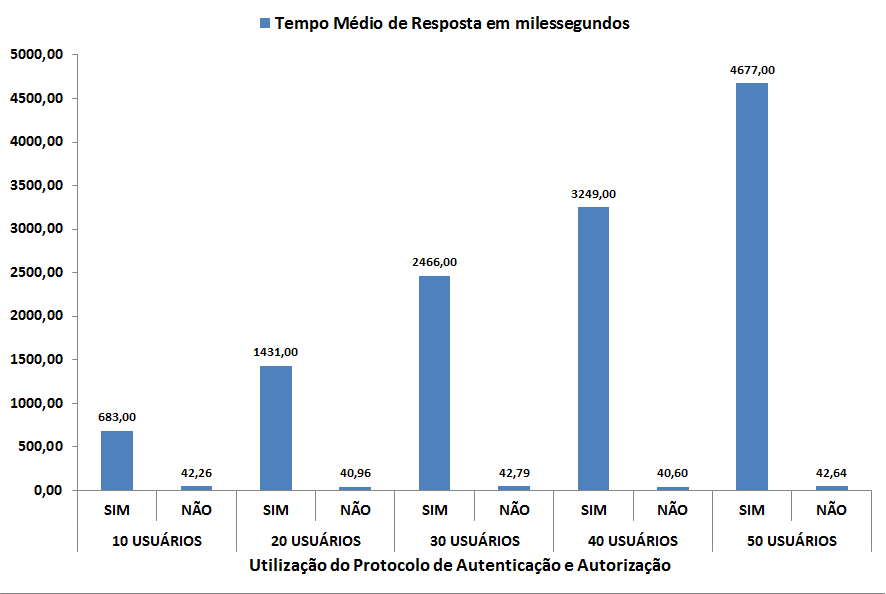
\includegraphics[width=1.0\textwidth]{grafico_teste_desempenho.png}
    \caption{Fluxo do protocolo de autenticação/autorização proposto, 1º cenário.}
    \label{fig:grafico_teste_desempenho}
\end{figure}


\section{Estudo de caso 2}\label{sec:caso2}

Os ambientes de teste utilizados foram o laboratório de informática da Universidade de Brasília e o da Divisão de Tecnologia da Policia Civil do Distrito Federal, uma vez que se busca resultados mais próximos da realidade hoje vivenciado pela PCDF.

Para a realização dos testes foram utilizadas configurações distintas de computadores, conforme apresentado na tabela~\ref{tb:estudo_caso2}.

Os web services adotados serão os mesmos definidos no estudo de caso 1, web service RESTfull de ocorrências criminais, que retornam informações gerais do sistema de ocorrências policiais.

\subsection{\emph{Configuração do ambiente de teste}}

Ambiente de teste foi o da Divisão de Tecnologia da Policia Civil do Distrito Federal, uma vez que se buscam resultados mais próximos da realidade hoje vivenciados pela PCDF.

Para a sua realização dos testes foram utilizados configurações distintas de computadores, conforme tabela abaixo. Essa configuração é idêntica a utilizada no estudo de caso 1.

%\begin{table}[!htpb]
%
%  \begin{tabular}{cp{13cm}}
\begin{table}[h]
    \begin{tabular}{|l|c|p{6cm}|}
    \hline
    \textbf{\emph{Máquina }}                   & \textbf{\emph{Quantidade}} & \textbf{\emph{Configuração}}                                                                               \\ \hline
    Servidor de Autenticação e Autorização  & 1          & Desktop DELL Intel Core I5-2450 2,5 GHz, 4 Gb RAM, 500 HD \\ \hline
    Servidor de Fachada REST  & 1          & Desktop DELL Intel Core I5-2450 2,5 GHz, 4 Gb RAM, 500 HD\\ \hline
    Cliente REST                   & 50        & Desktop DELL Intel Core I5-2450 2,5 GHz, 4 Gb RAM, 500 HD                                    \\ \hline
    \end{tabular}
    \caption {Ambiente de configuração estudo de caso 1}\label{tb:estudo_caso2}
\end{table}

Os servidores de Autenticação e Autorização, Fachada REST e Cliente REST, foram desenvolvidos utilizando a linguagem de programação funcional \emph{Haskell} acessando um banco de dados não relacional, \emph{Apache CouchDB}, conforme apresentado na seção~\ref{sec:implementacao}. O sistema operacional utilizado nessas máquinas foi o Linux Ubuntu 12.04 LTS-64 bits..

\subsection{\emph{Planejamento do experimento}}

O planejamento adotado neste estudo de caso procurou adaptar a realidade vivenciada na PCDF no oferecimento de um serviço. Desta forma, observou-se um cenário extremo de utilização, onde o número médio de requisições aos serviços RESTfull ofertados pela PCDF em 1 hora era de aproximadamente 1200 requisições, ou seja, uma média de duas requisições a cada segundo.

Sendo assim, objetiva-se verificar se o protocolo consegue atender um a caso extremo, que se assemelhe ao vivenciada pela PCDF. Logo, para simular esta situação, realizou-se um teste automatizado, utilizando a ferramenta Apache JMeter, que é um software open source, desenvolvido em Java.

Para realizar o experimento, a abordagem utilizada foi a da utilização de dois fatores: uso do protocolo de autenticação e autorização proposto (SIM/NÃO) e o número de usuários (50) com dois níveis e um nível respectivamente.  Para realizar o experimento foram realizadas 100 requisições para cada usuário, com um intervalo de 2 (dois) segundos de iniciação para cada usuário. As variáveis de resposta adotadas foram o tempo médio de resposta das requisições e a vazão média de requisições por segundo.

\subsection{Análise dos resultados}

A análise dos resultados obtidos com a execução do experimento ocorreu com a observação do tempo médio de resposta e com a verificação da vazão, número de requisições atendidas por segundo, que foi coletado ao final da execução do teste aplicado a um grupo de 50 usuários simultâneos. Dessa forma, foram coletadas 5000(cinco mil) amostras que utilizaram o protocolo de autenticação e autorização proposto em um período de 11 minutos. Os resultados estatísticos são apresentados na tabela~\ref{tb:estatistica_com_cripto_50}.

Em um cenário extremo, observou-se que a PCDF pode ter que responder a uma média de 1200 requisições de um serviço que fornece informações sobre ocorrências policiais em um período de 1 (uma) hora, ou seja, duas requisições a cada um segundo. Neste caso, os resultados obtidos com o experimento realizado com os 50 usuários simultâneos, demonstrou que o tempo médio de resposta foi de 4677 milessegundos ou aproximadamente 4,677 segundos e que a vazão média, que é o número de requisições atendidas por segundo, foi de 8,62 requisições por segundo. Ao se realizar a comparação deste cenário com o cenário extremo vivenciado pela PCDF, verificou-se que a arquitetura, do ponto de vista de vazão, atende perfeitamente o pior caso relatado, que é de 2 duas requisições por segundo. O que garante a qualidade do serviço ofertado pelo protocolo de autenticação e autorização proposto.

\begin{table}[h]
\centering
\begin{tabular}{|l|l|}
\hline
\textbf{Informação} & \textbf{Valor} \\ \hline
Nº de Requisições   &  5000              \\ \hline
Média               &  4677             \\ \hline
Mínimo              &  118          \\ \hline
Máximo              &  21665        \\ \hline
Desvio Padrão       &  3170,49      \\ \hline
\% Erro             &  0,0          \\ \hline
Vazão/seg           &  8,62     \\ \hline
Kbps                &  11,8         \\ \hline
Média de Bytes      &  1401,05      \\ \hline
\end{tabular}
\caption {Estatística básica com a utilização do protocolo de autenticação e autorização para 50 usuários.}\label{tb:estatistica_com_cripto_50}
\end{table}

\section{Síntese do capítulo}
Neste capítulo foram realizados dois estudos de caso, onde foram detalhados os cenários que seriam analisados, os ambientes e planejamento de testes e as referidas análises dos resultados obtidos.

Os estudos de casos realizados evidenciaram que o impacto no desempenho é significativo quando comparado com a não utilização da proposta. Porém os tempos médios obtidos estão dentro de um tempo médio esperado, que é abaixo de 5 segundos. Observou-se ainda, que em um cenário extremo de utilização, onde a PCDF tenha que atender a uma média de 2 duas requisições por segundo, e um período de 1 uma hora, ou seja 1200 requisições, a arquitetura proposta atende perfeitamente, pois consegue atender a 8,62 requisições por segundo em um cenário extremo onde foram realizados 5000 requisições em aproximadamente em 10 minutos. 
  % inserir demais capítulos

%\clearpage % this is need for add +1 to pageref of bibstart used in 'ficha catalografica'.
%\label{bibstart}
%\bibliography{reflatex} % geracao automatica das referencias a partir do arquivo reflatex.bib
%\label{bibend}

 \postextual
 \bibliographystyle{plain}
  %\bibliography{bibliografia}
  %\bibliography{bibliografia2}
 % \bibliography{reflatex}
   \bibliography{BibliografiaMPCA}
%\appendix
%  \chapter{Documentação Original}%
\small\begin{verbatim}
% -*- mode: LaTeX; coding: utf-8; -*-
%%%%%%%%%%%%%%%%%%%%%%%%%%%%%%%%%%%%%%%%%%%%%%%%%%%%%%%%%%%%%%%%%%%%%%%%%%%%%%%
%% File    : unb-cic.cls (LaTeX2e class file)
%% Authors : Flávio Maico Vaz da Costa
%%              (based on previous versions by José Carlos L. Ralha)
%% Version : 0.93
%% Updates : 0.5  [??/11/2004] - Initial release. don't remember the day.
%%         : 0.75 [04/04/2005] - Fixed font problems, UnB logo
%%                               resolution, keywords and palavras-chave
%%                               hyphenation and generation problems,
%%                               and a few other problems.
%%         : 0.8  [08/01/2006] - Corrigido o problema causado por
%%                               bancas com quatro membros. O quarto
%%                               membro agora é OPCIONAL.
%%                               Foi criado um novo comando chamado
%%                               bibliografia. Esse comando tem dois
%%                               argumentos onde o primeiro especifica
%%                               o nome do arquivo de referencias
%%                               bibliograficas e o segundo argumento
%%                               especifica o formato. Como efeito
%%                               colateral, as referências aparecem no
%%                               sumário.
%%         : 0.9 [02/03/2008]  - Reformulação total, com nova estrutura
%%                               de opções, comandos e ambientes, adequação
%%                               do logo da UnB às normas da universidade,
%%                               inúmeras melhorias tipográficas,
%%                               aprimoramento da integração com hyperref,
%%                               melhor tratamento de erros nos comandos,
%%                               documentação e limpeza do código da classe.
%%         : 0.91 [10/05/2008] - Suporte ao XeLaTeX, aprimorado suporte para
%%                               glossaries.sty, novos comandos \capa, \CDU
%%                               e \subtitle, ajustes de margem para opções
%%                               hyperref/impressao.
%%         : 0.92 [26/05/2008] - Melhora do ambiente {definition}, suporte
%%                               a hypcap, novos comandos \fontelogo e
%%                               \slashedzero, suporte [10pt, 11pt, 12pt].
%%                               Corrigido bug de seções de apêndice quando
%%                               usando \hypersetup{bookmarksnumbered=true}.
%%         : 0.93 [09/06/2008] - Correção na contagem de páginas, valores
%%                               load e config para opção hyperref, comandos
%%                               \ifhyperref e \SetTableFigures, melhor
%%                               formatação do quadrado CIP. 
%%
%% Definição de classe para dissertações do departamento de
%% Ciência da Computação (CIC) da Universidade de Brasília.
%%
%%%%%%%%%%%%%%%%%%%%%%%%%%%%%%%%%%%%%%%%%%%%%%%%%%%%%%%%%%%%%%%%%%%%%%%%%%%%%%%
%% PRÉ-REQUISITOS (usando LaTeX ou XeLaTeX):
%%
%% * Uma distribuição LaTeX2e compatível
%%   - em Windows, recomenda-se MiKTeX: http://miktex.org/
%% * Logomarca da UnB (arquivos positivo_cor.eps e contorno_preto.eps)
%%   - disponível na página: http://www.unb.br/unb/marca/index.php
%% * Pacotes obrigatórios
%%   - xkeyval, graphicx, boites, setspace,
%%     geometry, atbegshi, hyperref
%%
%% PRÉ-REQUISITOS (usando XeLaTeX):
%% * Fonte "Arial" instalada no sistema operacional
%% * Pacotes obrigatórios
%%   - fontspec, xltxtra (carregar no próprio documento)
%%
%% PRÉ-REQUISITOS (usando LaTeX):
%% * Fonte ua1 (URW Arial A030, PostScript Type-1)
%%   - disponível no CTAN: http://www.ctan.org/tex-archive/fonts/urw/arial/
%%   - no MiKTeX, basta instalar pacote "arial" via MiKTeX Package Manager
%% * Pacotes obrigatórios
%%   - relsize, fixltx2e
%% * Pacotes opcionais
%%   - MinionPro (fonte proprietária)
%%
%%%%%%%%%%%%%%%%%%%%%%%%%%%%%%%%%%%%%%%%%%%%%%%%%%%%%%%%%%%%%%%%%%%%%%%%%%%%%%%
%% PRINCIPAIS OPÇÕES DISPONÍVEIS:
%%
%% licenciatura - O trabalho é do curso de Licenciatura (Graduação).
%% bacharelado  - O trabalho é do curso de Bacharelado (Graduação).
%% mestrado     - O trabalho é de Mestrado.
%%
%% draft - Gera o documento em modo de rascunho: não exibe as imagens e
%%         modifica o espaçamento entre linhas.
%% final - Gera o documento em modo final, não-rascunho (padrão).
%%
%% impressao       - Gera a versão para impressão, sem hipertexto.
%% hyperref=load   - Carrega e configura o pacote hyperref para gerar
%%                   a versão hipertexto para exibição em tela (padrão).
%% hyperref=config - Configura o pacote hyperref para gerar
%%                   a versão hipertexto para exibição em tela, mas o
%%                   pacote deve ser carregado no próprio documento.
%%                   Leia a seção PROBLEMAS CONHECIDOS para recomendação
%%                   de uso desta opção.
%%
%% 10pt - Define tamanho da fonte do texto.
%% 11pt - Define tamanho da fonte do texto (padrão no modo draft).
%% 12pt - Define tamanho da fonte do texto (padrão no modo final).
%%
%% singlespacing  - Define espaçamento simples entre linhas (padrão no modo
%%                  final).
%% onehalfspacing - Define espaçamento de um e meio entre linhas (padrão no
%%                  modo draft).
%% doublespacing  - Define espaçamento duplo entre linhas.
%% baselineskip   - Utiliza o comando \baselineskip para definir o espaçamento
%%                  de linhas. Se não for infomada, o espaçamento é definido 
%%                  pelo pacote "setspace" (recomendável, ou seja, só use esta
%%                  opção se tiver algum motivo para não usar o setspace).
%%                  Pode ser usada em conjunto com uma das três opções acima.
%%
%% prestyle=<val>  - Especifica o estilo das páginas iniciais (agradecimentos,
%%                   resumo, sumário, etc.). Valores típicos são "plain"
%%                   (padrão) ou "empty".
%% textstyle=<val> - Especifica o estilo das páginas dos elementos textuais e
%%                   pós-textuais. Valores típicos são "plain" (padrão) ou
%%                   "fancy" (este último requer o pacote {fancyhdr}).
%% chapstyle=<val> - Especifica o estilo da primeira página de cada capítulo.
%%                   Valores típicos são "plain" (padrão) ou "empty".
%%
%%%%%%%%%%%%%%%%%%%%%%%%%%%%%%%%%%%%%%%%%%%%%%%%%%%%%%%%%%%%%%%%%%%%%%%%%%%%%%%
%% CRIAÇÃO DA MONOGRAFIA:
%%
%% A folha de rosto e folha de aprovação, por padronização estética,
%% são sempre formatados como "onehalfspacing" independente das opções
%% escolhidas. A seção de Referências é sempre "singlespacing". Citações
%% {quote}, {quotation} e versos {verse} são automaticamente "singlespacing" e
%% com letra menor.
%%
%% Os comandos \textlinf (lining figures) e \texttabf (tabular figures)
%% permitem selecionar, respectivamente, números "maiúsculos" (sim, isso
%% existe!) e números monoespaçados - o que só faz sentido para fontes 
%% que conhenham números maiúsculos x minúsculos e monoespaçados x
%% proporcionais (Minion Pro, Myriad Pro, Didot, Apple Chancery...).
%% Essas opção foi implementada apenas para a fonte Adobe Minion Pro no LaTeX,
%% mas funciona para qualquer fonte que suporte este recurso no XeLaTeX -
%% veja a documentação do pacote {fontspec} para mais informações.
%% Use \textlinf quando os números acompanharem texto em letras maiúsculas ou
%% em versalete (small-caps). Use \texttabf em tabelas ou outros lugares onde
%% for desejável que os números fiquem alinhados em colunas. Como alternativa
%% aos comandos, pode-se usar os ambientes {linfig} e {tabfig}.
%% O comando \SetTableFigures pode ser usado para redefinir um ambiente de
%% modo que os números contidos nele sejam automaticamente formatados
%% maiúsculos e monoespaçados, por exemplo: 
%%
%%   \SetTableFigures{tabular}
%%   \SetTableFigures{tabularx}
%%   \SetTableFigures{longtable}
%%
%% A capa, quando presente, não é contada na numeração das páginas.
%% As páginas iniciais, a partir da folha de rosto, são consideradas na 
%% contagem de páginas, mas não são numeradas.
%% As páginas seguintes (lista de figuras, etc.) por padrão são numeradas com
%% algarismos romanos e aparecem no sumário. Entretanto, se prestyle=empty,
%% não recebem numeração nem aparecem no sumário. 
%% As páginas do conteúdo (da introdução em diante) são numeradas com 
%% algarismos arábicos (13, 14, 15...) e começam a partir de 1.
%%
%% O sumário, por razões óbvias, deve colocado antes de todas as páginas
%% que são mencionadas nele.
%%
%% O trabalho é dividido em elementos pré-textuais, textuais e pós-textuais.
%% Estes elementos (alguns são opcionais, converse com seu orientador)
%% são dispostos preferencialmente na seguinte ordem:
%%    ELEMENTO                COMANDOS MAIS IMPORTANTES
%%       Capa                 \capa
%%    Elementos pré-textuais  \pretextual
%%       Folha de rosto       \folharosto
%%       Ficha catalográfica  \cip (impressa no verso da folha de rosto)
%%       Errata               %deve ser criada como documento avulso
%%       Folha de aprovação   \folhaaprovacao
%%       Dedicatória          \begin{dedicatoria}...\end{dedicatoria}
%%       Agradecimentos       \begin{agradecimentos}...\end{agradecimentos}
%%       Epígrafe             %aluno-poeta, esse recurso não está disponível
%%       Resumo               \begin{resumo}...\end{resumo}
%%       Abstract             \begin{abstract}...\end{abstract}
%%       Lista de Figuras     \figuras
%%       Lista de Tabelas     \tabelas
%%       Lista de Siglas      \printglossary[type=acronym] %usando pacote {glossaries}
%%       Sumário              \sumario
%%    Elementos textuais      \textual
%%       Introdução           \chapter{Introdu\c{c}\~ao} ...
%%       Desenvolvimento      \chapter{Nome do capitulo} \section{Nome da secao} ...
%%       Conclusão            \chapter{Conclus\~ao} ...
%%    Elementos pós-textuais  \postextual
%%       Referências          \bibliographystyle{...} \bibliography %usar BibTeX
%%       Glossário            \printglossary %usando pacote {glossaries}
%%       Apêndices            \apendices \chapter{Nome do apendice} ...
%%       Anexos               \anexos \chapter{Nome do anexo} ...
%%       Índices              \printindex %usando pacote {makeidx}
%%
%% O comando \maketitle equivale a chamar:
%% \pretextual\folharosto\cip\folhaaprovacao
%%
%% A opção "impressao", além de ajustar as margens para melhor
%% encadernação, também faz \maketitle chamar internamente o
%% comando \capa.
%%
%% Caso esteja preparando a versão para visualização em tela
%% (hipertexto), o documento pode ser configurado com o comando
%% \hypersetup a ser chamado no preâmbulo - mais detalhes no
%% manual do pacote hyperref. Algumas opções interessantes,
%% com valores de exemplo, são:
%%   bookmarksnumbered=true,
%%	   (itens das seções exibidas no menu do PDF são numerados)
%%   linktocpage=true,
%%	   (links do sumário nos números de página, não nos nomes de seções)
%%   colorlinks=true,
%%	   (indica links pela cor do texto, não por retângulo ao redor)
%%   linkcolor=red!80!black,
%%	   (cor de links em geral, veja pacote xcolor para opções de cor)
%%   urlcolor=blue,
%%	   (cor de links para URLs - comando \url{http://...})
%%   citecolor=teal,
%%	   (cor de links para referências citadas no texto)
%%   pdfstartview=FitH
%%	   (PDF exibido inicialmente com zoom para largura da página)
%%
%% O comando \listas equivale a chamar:
%% \figuras\tabelas
%%
%% O alinhamento e formatação dos títulos é controlado pelos comandos
%% \pretextual, \textual e \postextual, de modo que em cada parte do trabalho
%% os títulos são apresentados de maneira diferente. Se quiser mudar o
%% alinhamento do título numa das partes do trabalho, logo após a chamada ao
%% comando acima, redefina o comando \chapteralign para aplicar o alinhamento
%% desejado. Se quiser fazer outras mudanças no formato (por exemplo, colocar
%% os títulos em versalete (small-caps), será necessário redefinir o comando
%% \chapterformat (veja exemplo no código da classe).
%%
%% Redefina o comando \fontelogo para mudar o nome da fonte a ser utilizada
%% no logo da UnB, sendo que o padrão é "Arial" (XeLaTeX) ou "ua1" (LaTeX).
%% Deve-se trocar por uma fonte parecida (como a Helvetica, "phv" no LaTeX)
%% apenas se não for possível a instalação da Arial.
%%
%% A classe adicionalmente provê o ambiente {definition}, que exibe
%% definições (conceituais) numeradas e formatadas com borda.
%%
%% Alguns dos comandos a serem chamados no preâmbulo (parte do código antes
%% da chamada a \begin{document}) são:
%% \title[] - Título do trabalho.
%% \subtitle[] - Subtítulo do trabalho (se houver).
%% \palavraschave[] - Lista de palavras-chave em português.
%% \keywords[] - Lista de palavras-chave em inglês.
%%   Os parâmetros opcionais definem como o valor será apresentado na página
%%   da CIP e nas propriedades do PDF, já que estas não podem conter macros
%%   (ex.: \title[Um estudo sobre PI elevado a PI]{Um estudo sobre $\pi^\pi$}).
%% \diamesano - Dia mês e ano.
%% \autor - Nome e sobrenome do autor.
%% \coautor - Nome e sobrenome do co-autor (se houver).
%% \coordenador[a] - Coordenador(a) do curso.
%% \orientador[a] - Orientador(a) do trabalho.
%% \coorientador[a] - Coorientador(a) do trabalho (se houver).
%% \membrobanca - Adiciona membros à banca (além do orientador e coorientador).
%% \CDU - Classificação Decimal Universal (por padrão é 004).
%%   Valores comuns para a área (conforme http://www.udcc.org/) são:
%%    004 Ciência da Computação e Tecnologia
%%    004.2	Arquitetura de computadores
%%    004.3	Hardware
%%    004.4	Software
%%    004.5	Interação homem-máquina
%%    004.6	Dados
%%    004.7	Comunicação de computadores
%%    004.8	Inteligência artificial
%%    004.9	Técnicas de informática orientadas a aplicação
%%
%%%%%%%%%%%%%%%%%%%%%%%%%%%%%%%%%%%%%%%%%%%%%%%%%%%%%%%%%%%%%%%%%%%%%%%%%%%%%%%
%% PROBLEMAS CONHECIDOS:
%%
%% * O pacote hyperref, embora muito útil para gerar um PDF para leitura em
%%   tela, tem inúmeros problemas de compatibilidade com outros pacotes -
%%   alguns só funcionam corretamente se forem carregados antes do hyperref.
%%   A opção [hyperref] (ou seu sinônimo [hyperref=load]) carregam o pacote
%%   na própria classe, o que impossibilita que algum pacote no documento do
%%   aluno seja carregado antes do hyperref. Neste caso, usar a opção
%%   [hyperref=config] junto com o comando \ifhyperref para carregar o
%%   hyperref apenas quando estiver sendo gerada uma versão para leitura em
%%   tela, como no seguinte exemplo:
%%
%%     %%% não carrega nameref com opção [impressao] 
%%     \ifhyperref{\usepackage{nameref}}{}
%%     %%% varioref só funciona se carregado entre nameref e hyperref
%%     \usepackage{varioref}
%%     %%% não carrega hyperref com opção [impressao] 
%%     \ifhyperref{\usepackage{hyperref}}{}
%%
%% * Recomenda-se o uso do XeTeX ou pdfTeX, já que o dvips (+ps2pdf)
%%   não suporta adequadamente links com quebra de linha. Quem deseja usar os
%%   recursos gráficos do PSTricks pode experimentar o pacote TikZ como
%%   alternativa que não depende de diretivas PostScript.
%% * O suporte para o modo matemático ainda não está completo no XeTeX. Se seu
%%   trabalho depende significativamente de fórmulas e equações, use o LaTeX
%%   (ou XeLaTeX com \usepackage[no-math]{fontspec} e uma fonte matemática do
%%   LaTeX que combine com a fonte escolhida para o texto).
%%
%%%%%%%%%%%%%%%%%%%%%%%%%%%%%%%%%%%%%%%%%%%%%%%%%%%%%%%%%%%%%%%%%%%%%%%%%%%%%%%
%% ORIENTAÇÕES TIPOGRÁFICAS:
%%
%% * Atenção aos diferentes tipos de traço:
%%      - O hífen (-) liga prefixos, sufixos, partículas e pronomes oblíquos
%%        (ex.: recordar-se, fazê-lo, co-habitar).
%%      - A meia-risca (--) indica intervalos numéricos e liga palavras
%%        independentes (ex.: páginas 1--5, viagem Londres--Estocolmo, São João
%%        del-Rei--MG).
%%      - O travessão (---) é usado em diálogos, quando o interlocutor muda,
%%        e pode substituir dois pontos, parênteses ou vírgulas em apostos.
%%   Antes e depois de travessão emprega-se espaço, nos demais casos não há 
%%   espaço.
%% * O ponto final marca o fim de uma sentença. Se o ponto for usado com outra
%%   finalidade, como numa abreviatura, usar \ (ou ~ se não quiser permitir 
%%   quebra de linha) para indicar ao TeX que não se trata de fim de sentença
%%   (ex.: Dr.\ Spock).
%% * Embora o padrão das normas ABNT (que, com suas "receitinhas de bolo", são
%%   bastante rudimentares quanto à tipografia) seja espaçamento duplo entre 
%%   linhas, o espaçamento deve ser escolhido de acordo com o tipo e tamanho
%%   das letras.
%%   A regra a ser seguida é: quanto maiores as linhas (quanto mais palavras
%%   por linha), maior deve ser o espaçamento entre elas. Muitas vezes o
%%   espaçamento simples é suficiente numa fonte bem elaborada, mas se o
%%   tamanho médio da linha for superior a 90 caracteres, pode-se aumentar a
%%   legibilidade definindo um modesto incremento de espaçamento (algo entre
%%   \SetSinglespace{1.1} e \SetSinglespace{1.15}).
%% * Como um trabalho acadêmico tem margens relativamente estreitas, para
%%   evitar que as linhas sejam muito longas, em modo final esta classe utiliza
%%   tamanho 12pt.
%%   Deve haver interesse nas opções 10pt ou 11pt apenas se estiver sendo
%%   utilizada uma fonte particularmente grande (por exemplo, que produza uma
%%   média inferior a 80 caracteres por linha a 12pt).
%% * Na tipografia brasileira e portuguesa é costume recuar (indentar) a
%%   primeira linha de cada parágrafo. Como esse recuo serve para destacar
%%   visualmente um parágrafo de seu anterior, o LaTeX não faz o recuo no
%%   primeiro parágrafo sob um título. Quem quiser indentar também o primeiro
%%   parágrafo só para "manter o costume" deve adicionar o pacote {indentfirst}
%%   ao seu documento.
%% * Citações com até três linhas ficam no próprio texto, marcadas por "aspas".
%%   Se o texto original contiver "aspas", trocá-las por 'aspas simples'.
%%   Se a citação tiver mais de três linhas e apenas um parágrafo, usar o
%%   ambiente {quote}. Se a citação tiver mais de um parágrafo, usar
%%   {quotation}. Nestes dois casos, não se deve circundar sua citação por
%%   aspas nem alterar as aspas do texto original.
%%   Se a citação começar com letra maiúscula, o texto imediatamente anterior
%%   deve terminar em dois pontos (:).
%% * Números ordinais em inglês são sucedidos por "st", "nd", "rd" ou "th",
%%   de acordo com o seguinte algoritmo:
%%      Se o número termina em 1 mas não termina em 11, use "st".
%%      Se o número termina em 2 mas não termina em 12, use "nd".
%%      Se o número termina em 3 mas não termina em 13, use "rd".
%%      Em quaisquer outros casos, use "th".
%%   Esse indicador de ordinal deve, preferencialmente, ser colocado como texto
%%   superscrito. Usar 112\textsuperscript{th} e não 112$^{th}$. Se não quiser
%%   se preocupar com essas regras, use o pacote {engord} com o comando
%%   \engordnumber{112}.
%% * Para indicar elipse (reticências), use \textellipsis,
%%   usar ... (ponto ponto ponto) não é a mesma coisa.
%%
%%%%%%%%%%%%%%%%%%%%%%%%%%%%%%%%%%%%%%%%%%%%%%%%%%%%%%%%%%%%%%%%%%%%%%%%%%%%%%%
%% FIM DA DOCUMENTAÇÃO
%%%%%%%%%%%%%%%%%%%%%%%%%%%%%%%%%%%%%%%%%%%%%%%%%%%%%%%%%%%%%%%%%%%%%%%%%%%%%%%
\end{verbatim}

\end{document}
